\documentclass[12pt,a4paper]{article}
%Chargement des packages
\usepackage[utf8]{inputenc} % l'encodage des fichiers est utf-8, mettre [latin1] si necessaire
\usepackage[english]{babel} %le rapport est en français 
\usepackage{amsmath}
\usepackage{amsfonts}
\usepackage{amssymb}
\usepackage{graphicx} %pour afficher des images
\usepackage{float}	%pour forcer le placement des images.
\usepackage{geometry} %pour la modification des marges
\usepackage{fancyhdr} %pour modification des pieds de page
\usepackage{longtable}
\usepackage{listings}
%\usepackage{subfigure}
\usepackage{hyperref} %pour que les références soient des liens hypertextes
\usepackage[usenames,dvipsnames]{color} % pour les textes en gris
\usepackage{bm}
\usepackage{wrapfig}
\usepackage{caption}
\usepackage{subcaption}
%\usepackage{draftwatermark}
%\SetWatermarkScale{5}
\usepackage{varwidth,xcolor}

\newcommand{\authorDoc}{Prénom Nom}
\newcommand{\wvec}[1]{\ensuremath{\overrightarrow{#1}}}
% Comment utiliser : 
% - la page de titre est à personnaliser (title/title.tex)
% - le contenu est à rédiger dans le répertoire pages/, s'inspirer des exemples présents dans ce modèle.
% - les annexes sont à rédiger dans le répertoire appendix/
% - la bibliographie utilise BibTex (fichier biblio.bib)
% - les variables suivantes sont à remplir :

\newcommand{\TitreRapport}{Tema 2-3. Problemas de difusión estacionarios.}
\newcommand{\DateRapport}{8-9 Febrero 2023}
\newcommand{\AuteurRapport}{Grupo Mecánica Computacional}
\newcommand{\NomEntreprise}{Máster en Ing. de Caminos, Canales y Puertos}

%définition des marges
\geometry{hmargin=2.5cm, vmargin=2.5cm } 

%utilisation des puces anglaises.
%attention, il faut avoir une version récente de frenchb.ldf. 
%\frenchbsetup{StandardItemLabels}

%Définition des en-têtes et pieds de page
\renewcommand{\headrulewidth}{0pt}
\renewcommand{\footrulewidth}{0pt}
\fancyhead[C]{ \textcolor{Gray}{\small\TitreRapport}}
\fancyfoot[C]{ \textcolor{Gray}{ \small\AuteurRapport ~~ \vline ~~ Prácticas MCIC ~~ \vline ~~ \DateRapport }}

\fancyfoot[LE, RO]{\thepage}
\fancyfoot[RE, LO]{
\includegraphics[width=1.8cm]{style/images/logo_small.png}}

\fancyhead[L,R]{}


% définition du tire, de la date et de l'auteur du document
\title{\TitreRapport}
\date{\DateRapport}
\author{\AuteurRapport}


\makeatletter

\renewcommand\maketitle{
  \begin{titlepage}
  	\begin{center}
    	
\includegraphics[width=3.0cm]{title/images/logo_UPM.jpg}
    	\hspace{\stretch{1}}
    	
\includegraphics[width=2.5cm]{title/images/EtsiCam.pdf}
    
    \vspace{\stretch{0.5}}
    	
		  \begin{tabular*}{1.0\textwidth}{l @{\extracolsep{\fill}} r}
					Universidad Politécnica de Madrid 				& \NomEntreprise 				\\
%					TFE \@date 							& Ville du lieu du Stage 		\\
			\end{tabular*}

  	\vspace{\stretch{1.5}}
  		{\large \bf Computational Methods in Civil Engineering. Practical cases. \\}
    \vspace{0.5cm}
    {\LARGE \bf \@title\\}
    \vspace{0.5cm}
    {\large \it \@author\\}
  
	  \vspace{\stretch{2}}
	  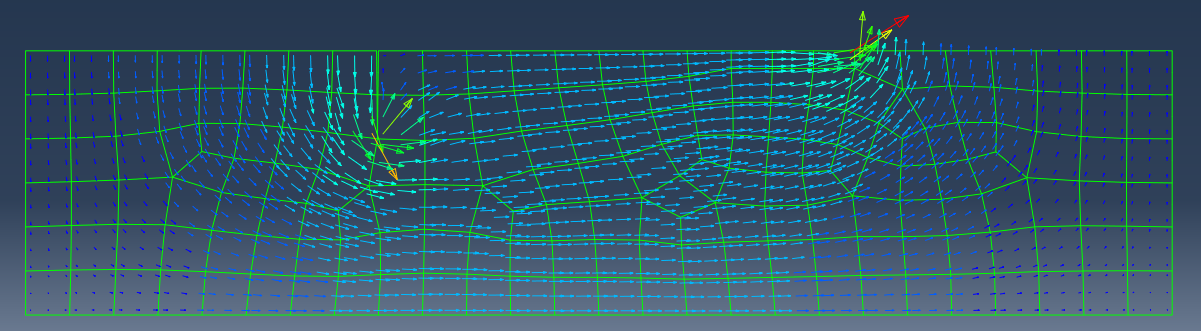
\includegraphics[width=0.95\textwidth]{title/images/bc1.jpg}
	  \vspace{\stretch{2}}
	    
		  % \begin{tabular*}{1.0\textwidth}{|l @{\extracolsep{\fill}} r|}
		  %       	\hline
		  %       		&\\
		  %       		\textit{ALUMNO} :&\\
		  %       		& \\
		  %       	        \textit{FECHA DE ENTREGA}:&\\
		  %       		&\\	
		  %       	\hline
		  %       \end{tabular*}
		\end{center}\par
    
  \end{titlepage}
  \setcounter{footnote}{0}
  
%  \global\let\thanks\relax
%  \global\let\maketitle\relax
%  \global\let\@thanks\@empty
%  \global\let\@author\@empty
%  \global\let\@date\@empty
%  \global\let\@title\@empty
%  \global\let\title\relax
%  \global\let\author\relax
%  \global\let\date\relax
%  \global\let\and\relax
}


\makeatother


\begin{document}
\pagestyle{fancy}
     
\maketitle
% \newpage \section*{Remerciements}
Insérez ici vos remerciements.
 \newpage
% \section*{Résumé du rapport :}
Insérez ici le résumé en français

\subsubsection*{Mots-clés libres :}
Insérez ici les mots clés en français (séparés par des points-virgules)
 \newpage
% \section*{Abstract:}
Insérez ici le résumé en anglais

\subsubsection*{Keywords:}
Insérez ici les mots clés en anglais (séparés par des points-virgules)
 \newpage
% \tableofcontents
% 
% \newpage \listoffigures \listoftables \newpage
\section*{Introduction}
\addcontentsline{toc}{section}{Introduction} The goals of this
practice are:
\begin{enumerate}
\item Reinforce the practical concepts associated with (i) the
  numerical analysis by the finite element method and (ii) the use of
  the Abaqus program.
\item Review the problem of stationary diffusion, its numerical
  resolution and apply these concepts to the problem of fluid flow in a porous
  medium.
\end{enumerate}

The practice consists of three sections:
\begin{description}
\item[Section 1.] Brief introduction to the problem of steady-state fluid flow in a
  porous medium.
\item[Section 2.] Description of the finite element analysis procedure
  of a steady state diffusion problem with the Abaqus program.
\item[Section 3.] Four exercises to be solved by the student.
\end{description}
\clearpage
 \newpage

% \section{Introduction to Numerical Analysis with Abaqus}

\subsection{Motivation}

\paragraph{Introduction to the Abaqus program.} Abaqus is a program
(or suite of programs) to perform finite element analysis with two
ways of working:
\begin{enumerate}
\item \textbf{Interactive:} Using the graphical user interface Abaqus/CAE (look at Fig.~\ref{figu10}).
  \begin{itemize}
  \item It is not necessary to learn the syntax of the program's input
    file.
  \item It is more laborious to change a parameter and perform a new 
    analysis.
  \end{itemize}
  \begin{figure}[!h]
    \begin{center}
      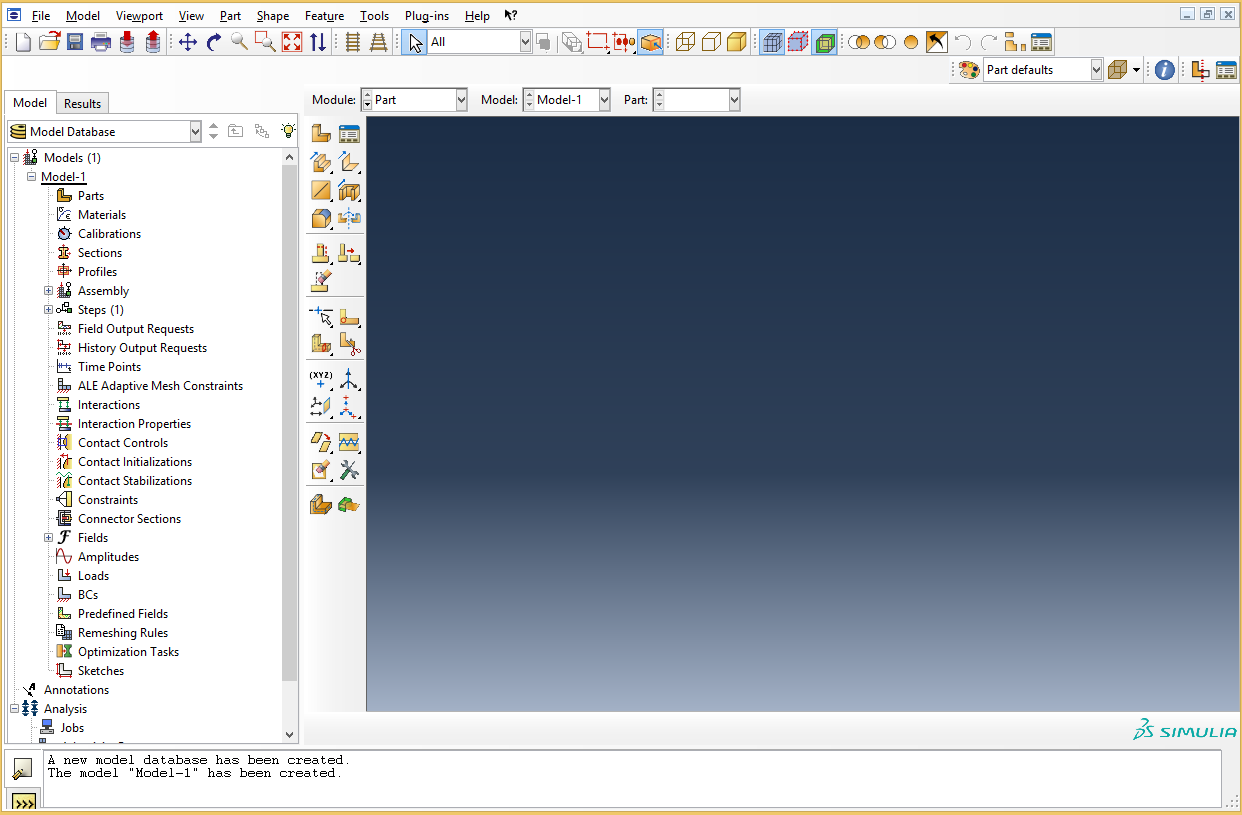
\includegraphics[width=0.9\textwidth]{./body/images/imagen10}
    \end{center}
    \caption{Abaqus/CAE graphic interface}
    \label{figu10}
  \end{figure}
\item \textbf{Keywords:} Writing a plain text input file \texttt{.inp}
  with the commands needed to perform the analysis (look at
  Fig.~\ref{figu09}).
  \begin{itemize}
  \item You must know the syntax of the program's input file.
  \item It is very easy to modify something and perform a new
    analysis.
  \item Although we work in \textit{interactive} mode, at the end
    Abaqus always generates a plain text file.
  \end{itemize}
  \begin{figure}[!h]
    \begin{center}
      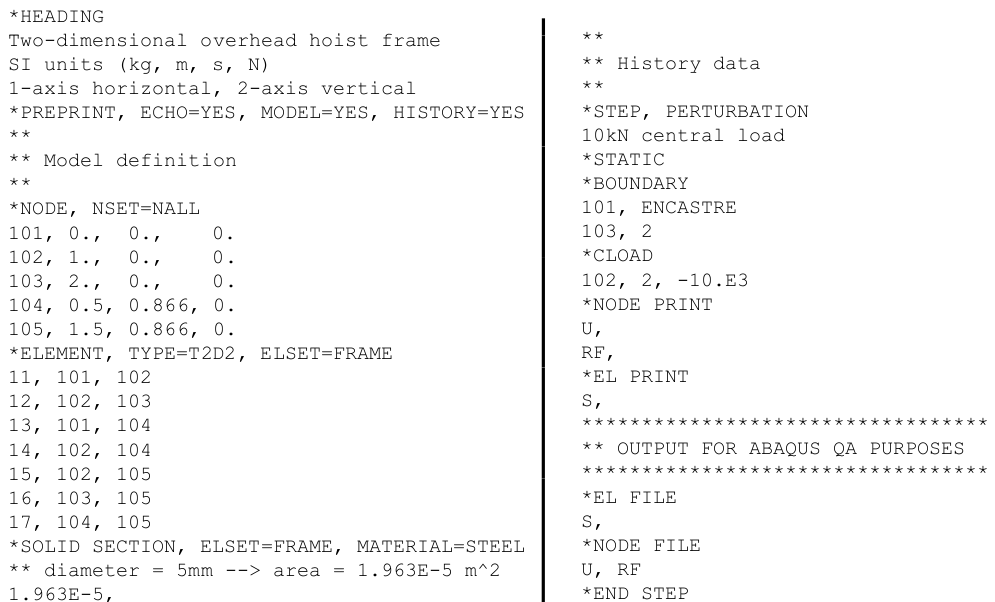
\includegraphics[width=0.8\textwidth]{./body/images/imagen09}
    \end{center}
    \caption{Example .inp file}
    \label{figu09}
  \end{figure}
\end{enumerate}

We are going to work in this course in \textit{interactive} mode. To start The
Abaqus/CAE graphic preprocessing program we must write \textbf{abaqus
  cae} at the command console or click the direct link in the
computer.  Once started, among the options the program gives us we
choose \textbf{Create Model Database with Standard/Explicit Model} as
indicated in Fig.~\ref{figu00}).
\begin{figure}[!h]
  \begin{center}
    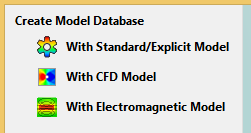
\includegraphics[width=0.4\textwidth]{./body/images/imagen00}
  \end{center}
  \caption{Start of the program Abaqus}
  \label{figu00}
\end{figure}

We have the Abaqus/CAE working environment where we can identify the
following sections (look at Fig.~\ref{figu11}):
\begin{itemize}
\item \textit{Viewport:} Main part of the Abaqus/CAE screen where we
  visualize the pre and post processing of our analysis.
\item \textit{Model Tree View:} All the steps we follow in our model
  (everything we define on it) are represented in this area in the
  form of tree nodes. Each node is subdivided into several subnodes
  with their corresponding functionalities.  If the \textit{Model
    Tree} is not visible, make it visible by pressing
  \textbf{View/Show Model Tree} or pressing \texttt{CTRL+T}.
\item \textit{Toolbar Section:} Each node of the \textit{Model Tree}
  corresponds to a toolbar where the user can access the associated
  commands. We can access these commands also through the drop-down
  menus of the top bar (although in this tutorial we will use the
  graphic icons of the toolbar).
\item \textit{Prompt region:} When we select a certain command,
  information about the next action to be performed appears in the
  \textit{Prompt} region.
\end{itemize}

\begin{figure}[!h]
  \begin{center}
    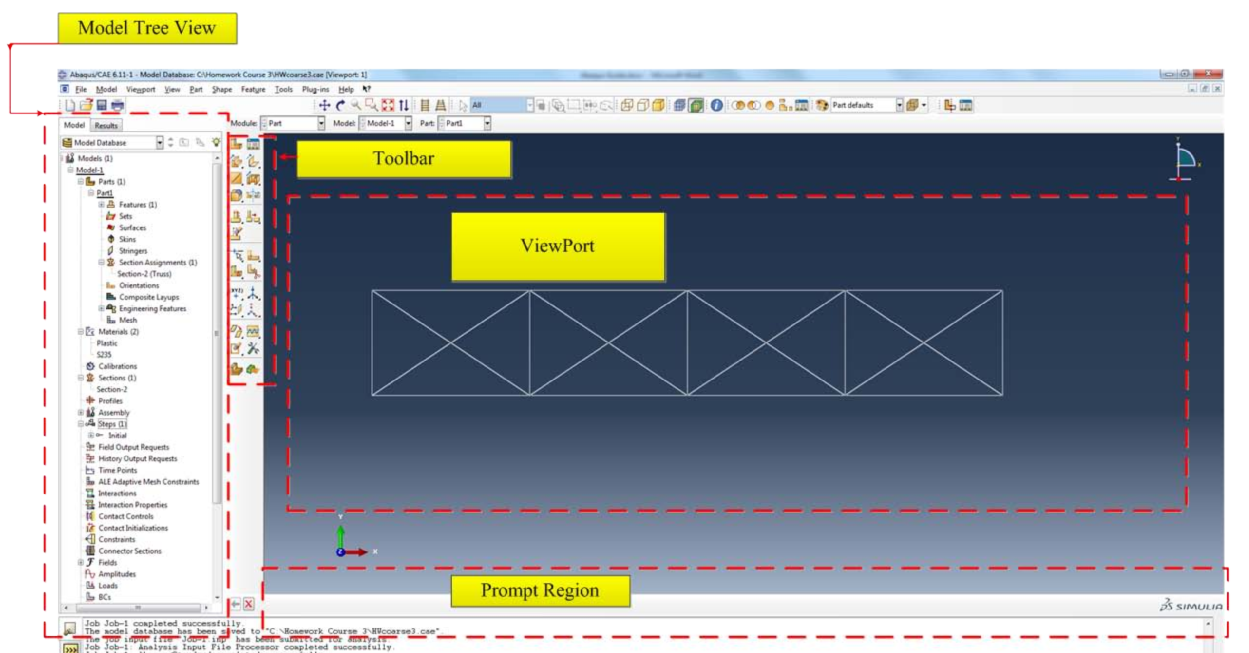
\includegraphics[width=1.05\textwidth]{./body/images/imagen11}
  \end{center}
  \caption{Abaqus/CAE working space description}
  \label{figu11}
\end{figure}




\paragraph{Stages of analysis} To carry out a finite element analysis, we must perform a series of steps. Abaqus has grouped these steps into \textbf{Modules} sequentially. The functionalities associated with each module 
\footnote{Modules with an asterisk * will not to be used in this course} is summarized now:
\begin{description}
\item[Module Part.] Create the geometry of the domain's elements.
  (\textit{Parts})
  \begin{enumerate}
  \item Sketch the geometry   of the domain's elements.      
  \item Create \textit{Parts} with the geometry   of the domain's elements.
  \end{enumerate}
  
\item[Module Property.] Define materials and sections.
  \begin{enumerate}
  \item Define the properties of the materials.
  \item Define the sections (which we associate with the materials).
  \item Assign the sections to the corresponding \textit{Parts}.
  \end{enumerate}
\item[Module Assembly.] Assemble the model by creating copies (instances) of the \textit{Parts}.
\item[Module Step.] Set the analysis procedure.
  \begin{enumerate}
  \item Define calculation steps
  \item Define the type of analysis in each calculation step (thermal, mechanical, stationary, transient, \ldots)
  \item Define the variables that the program must save to display in the post process.
  \item Define the parameters of the numerical algorithms used in each calculation step.
  \end{enumerate}
\item[Module Interaction*.] Create constraints between elements of our geometry.
\item[Module Load.] 
Apply the boundary conditions at each step of time.
\item[Module Mesh.] Create the mesh.
\item[Module Optimization*.] Use finite element analysis to optimize a property of our model.
\item[Module Job.] Create the job and launch the numerical analysis.
\item[Module Visualization.] Perform the post-process.
\end{description}
 


\paragraph{Description of the problem to be solved.} One of the first
things we must do before building the numerical model is to decide
which system of units we are going to use. Abaqus does not have a
predefined system, we simply have to work on a consistent unit
system. In Fig.~\ref{figu01} four systems of consistent units are
shown:
\begin{figure}[!h]
  \begin{center}
    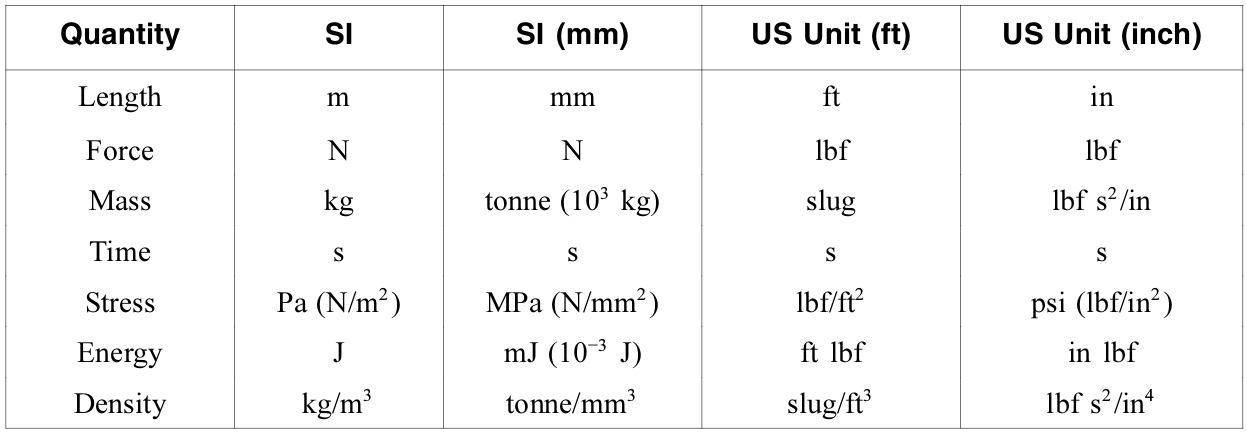
\includegraphics[width=0.9\textwidth]{./body/images/imagen01}
  \end{center}
  \caption{Consistent unit systems}
  \label{figu01}
\end{figure}

The problem we want to solve is summarized in Fig.~\ref{figu114}.  It
is a beam clamped in its left end that has a tension vector
$\mathbf{t}^*=[0,-1000,0]^T$ Pa applied to the right half of its upper
face. The measures of the beam are 5 meters in length and a square
section of 1 meter in side. The material is concrete with elastic
constants $E=27$ GPa and $\nu=0.3$. As you can see, our problem can be
reduced to a 2D problem in plane stress.

\begin{figure}[!h]
  \begin{center}
    \includegraphics[width=0.9\textwidth]{./body/images/imagen114}
  \end{center}
  \caption{Description of model}
  \label{figu114}
\end{figure}



\paragraph{Starting of the analysis with Abaqus.} Before starting to work
let us do three things:
\begin{enumerate}
\item Defining a working directory in \textbf{File/Set Work Directory}
  where all the files we generate will be saved.
\item See help from Abaqus:
  \begin{itemize}
  \item If you go to \textbf{Help/On Context} we will get help on the
    icon (command) that we click afterwards.
  \item If you go to \textbf{Help/On Module} we will get help on the
    module you are in at the moment.
  \item If you go to \textbf{Help/Search and Browse Guide} we will go
    to the main page of Abaqus help.
  \end{itemize}
\item We assign a name to our model. Place the cursor over the model
  at the top of the \textit{Model Tree}, right click the mouse, select
  \textbf{Rename} and assign it the name \textit{Mensula}. Be sure you
  obtain something like Fig.~\ref{figu12}.
  \begin{figure}[!h]
    \begin{center}
      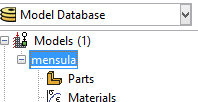
\includegraphics[width=0.3\textwidth]{./body/images/imagen12}
    \end{center}
    \caption{Change of the model's name}
    \label{figu12}
  \end{figure}
\end{enumerate}

In the remaining of this chapter we will describe all the phases of
the numerical analysis by using the example described in
Fig.~\ref{figu114}.

\newpage
\subsection{Module Part. Create the geometry of the domain's
  elements.}
In Abaqus we must define the geometry of the elements that form our
model. These elements are called \textit{parts} and will allow us to
assemble a model by creating one or more copies (instances) of each
\textit{part}, in case there are repeated elements.

In order to define the geometry of the elements of our model:
\begin{enumerate}
\item We activate module \textbf{Part} and we press command
  \textbf{Create Part} (look at Fig.~\ref{figu02}).

  In the lower left corner Abaqus shows a message (Prompt) that tells
  us what to do (in this case ``\textit{Fill out the Create Part
    dialog}''. Press the \textbf{Cancel} button to cancel the task we
  are doing, the \textbf{Previous} button to cancel the step we are
  doing inside a task and return to the previous step and the
  \textbf{Done} button to finish the task (see Fig.~\ref{figu03}).

\begin{figure}[H]
  \centering
  \begin{subfigure}{0.25\textwidth}
    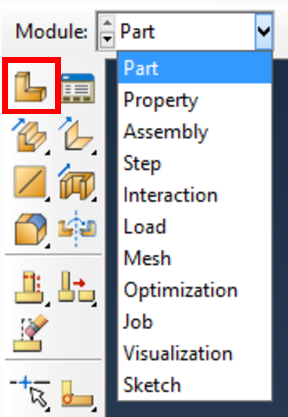
\includegraphics[width=\textwidth]{./body/images/imagen02.pdf}
    \caption{Command \textbf{Create Part}}
    \label{figu02}
  \end{subfigure}%
  ~ %add desired spacing between images, e. g. ~, \quad, \qquad, \hfill etc.
  % (or a blank line to force the subfigure onto a new line)
  \begin{subfigure}{0.65\textwidth}
    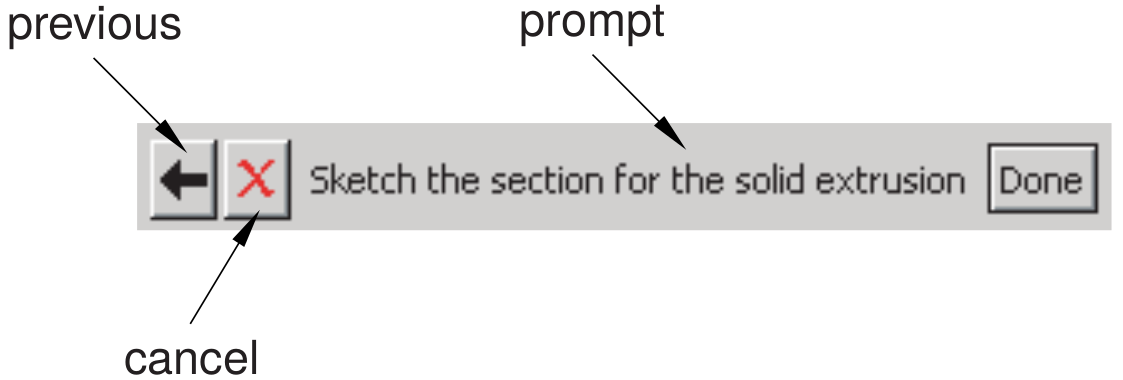
\includegraphics[width=\textwidth]{./body/images/imagen03}
    \caption{Message informing action}
    \label{figu03}
  \end{subfigure}
  \caption{Onset of module \textit{Part} and \textit{Prompt} message
    of information}
\end{figure}

We see now the dialog \textbf{Create Part} where we are asked if our
model is going to be a three-dimensional, 2D planar or axisymmetric
domain (\textbf{modeling space}), if it is going to be a deformable or
rigid object (\textbf{Type}) and what type of geometry is
(\textbf{Base Feature}). For our problem we will choose the options
indicated in Fig.~\ref{figu04}.  We put a value of 10 (meters in our
assumed unit system) in the variable \textbf{Approximate size}, which
is double the maximum dimension of our domain. With this dimension
Abaqus will provide us with a working environment where we can create
the geometry.


\begin{figure}[!h]
  \begin{center}
    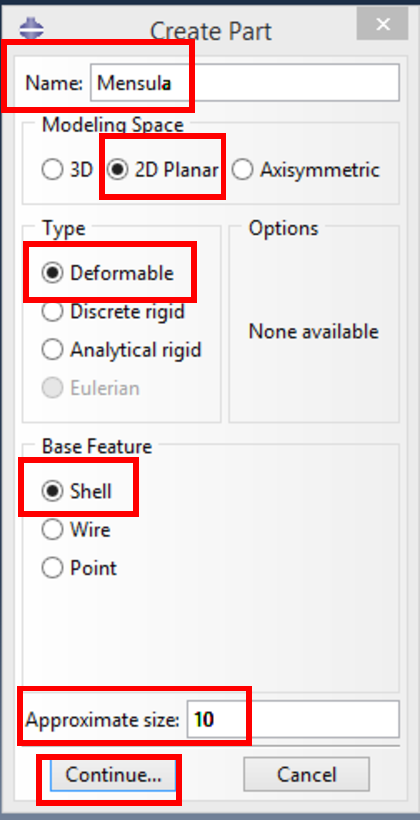
\includegraphics[width=0.35\textwidth]{./body/images/imagen04.pdf}
  \end{center}
  \caption{Dialog \textbf{Create Part}}
  \label{figu04}
\end{figure}

\item Next we get a screen of a working environment
  (\textit{Sketcher}) with the CAD tools needed to create the geometry
  of our \textit{part}. Regarding the sketcher we must know:
  \begin{itemize}
  \item You can use the points of the working window (by clicking the
    mouse) to define geometric entities.
  \item Dotted lines are the X and Y axes and intersect at the origin.
  \item The orientation of the work plane is defined with the axes at
    the bottom left.
  \item When you activate a drawing tool, the coordinates are drawn in
    the upper left.
  \end{itemize}

  There are two ways to define this geometry: (a) define the geometric
  entities precisely and (b) define them quickly using the grid and
  then apply constraints to achieve the desired geometry. Let's work
  the second way:
  \begin{enumerate}
  \item Press the \textbf{Create lines: Rectangle} button and draw a
    rectangle without worrying about the dimensions (see
    Fig.~\ref{figu05}).
    \begin{figure}[!h]
      \begin{center}
        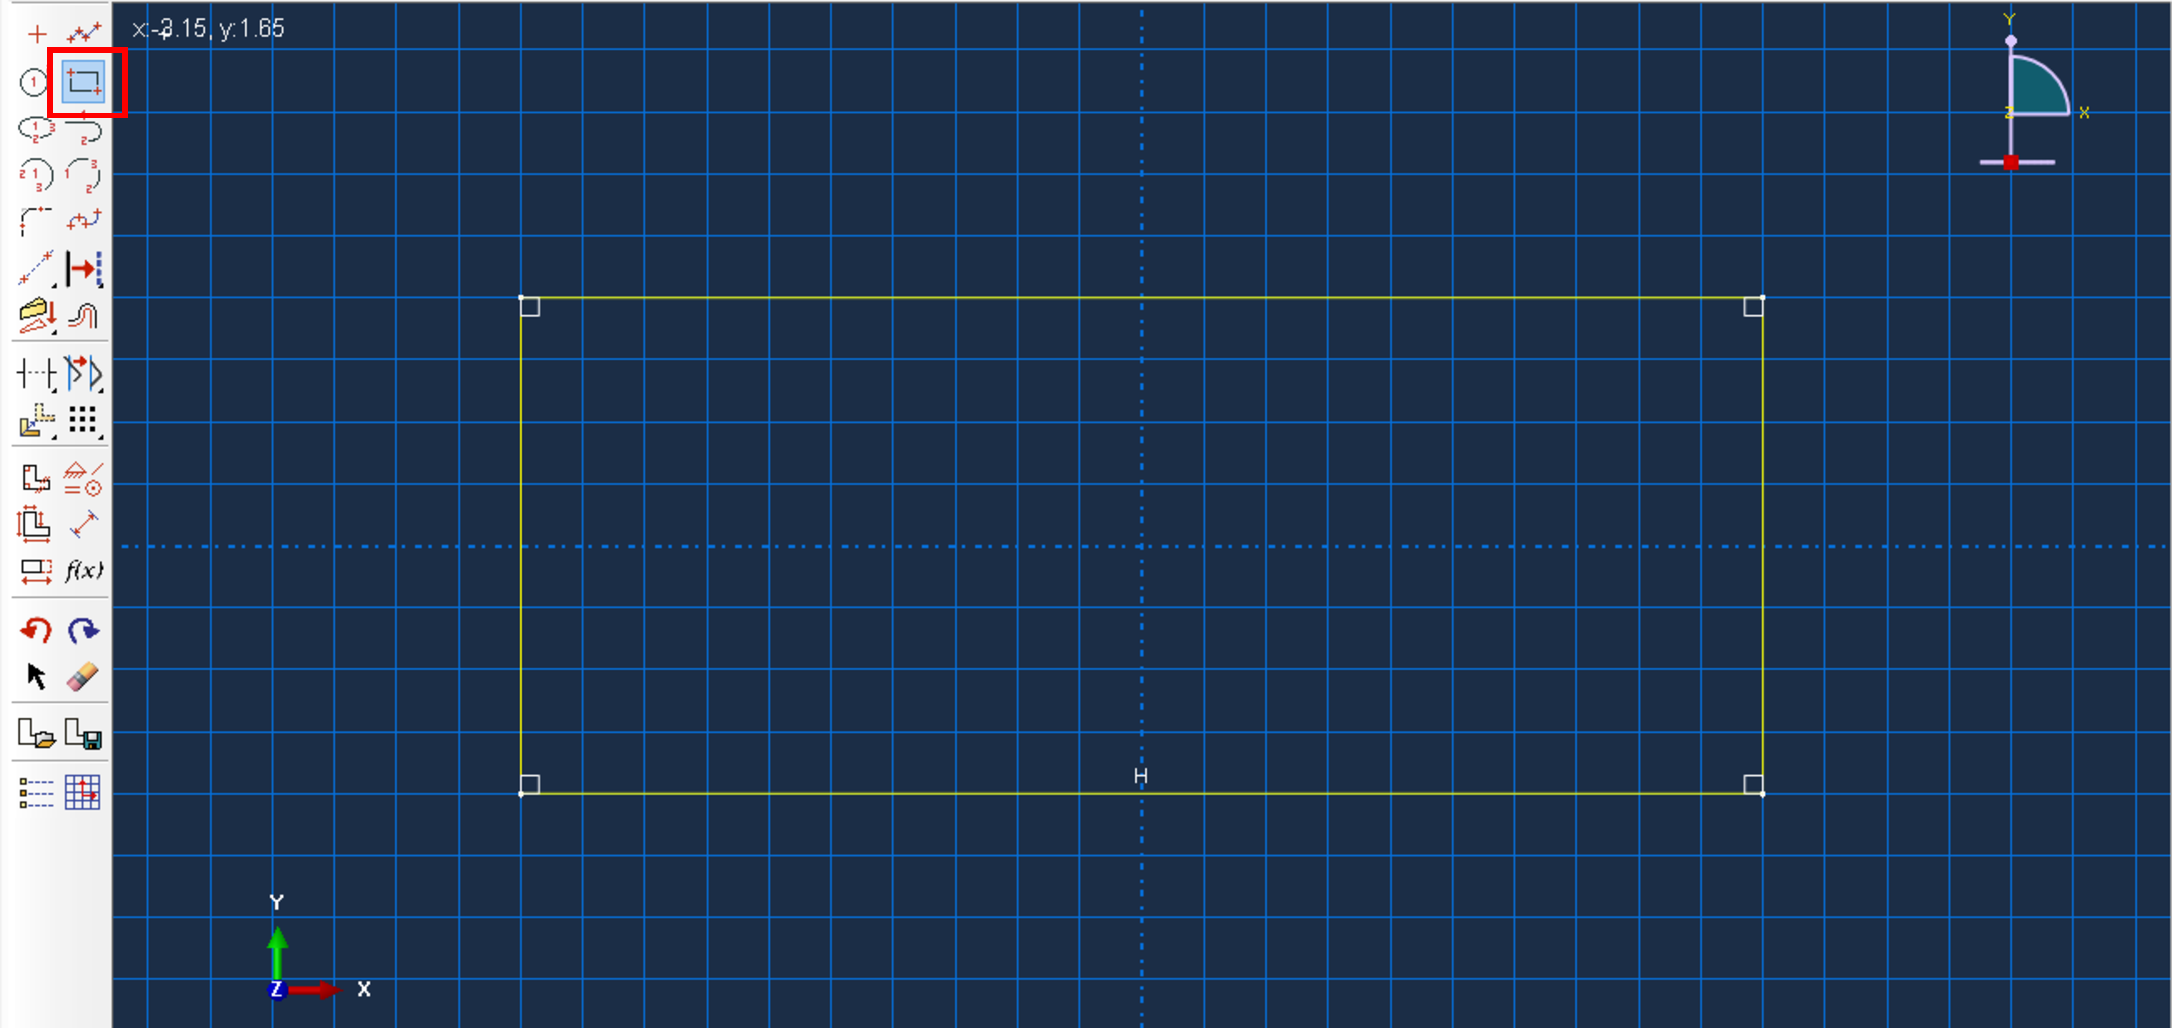
\includegraphics[width=0.875\textwidth]{./body/images/imagen05.pdf}
      \end{center}
      \caption{Initial Rectangle}
      \label{figu05}
    \end{figure}

  \item Press the command \textbf{Add dimension}, select one of the
    horizontal sides and modify the dimension to 5 meters (see
    Fig.~\ref{figu06}).
    \begin{figure}[!h]
      \begin{center}
        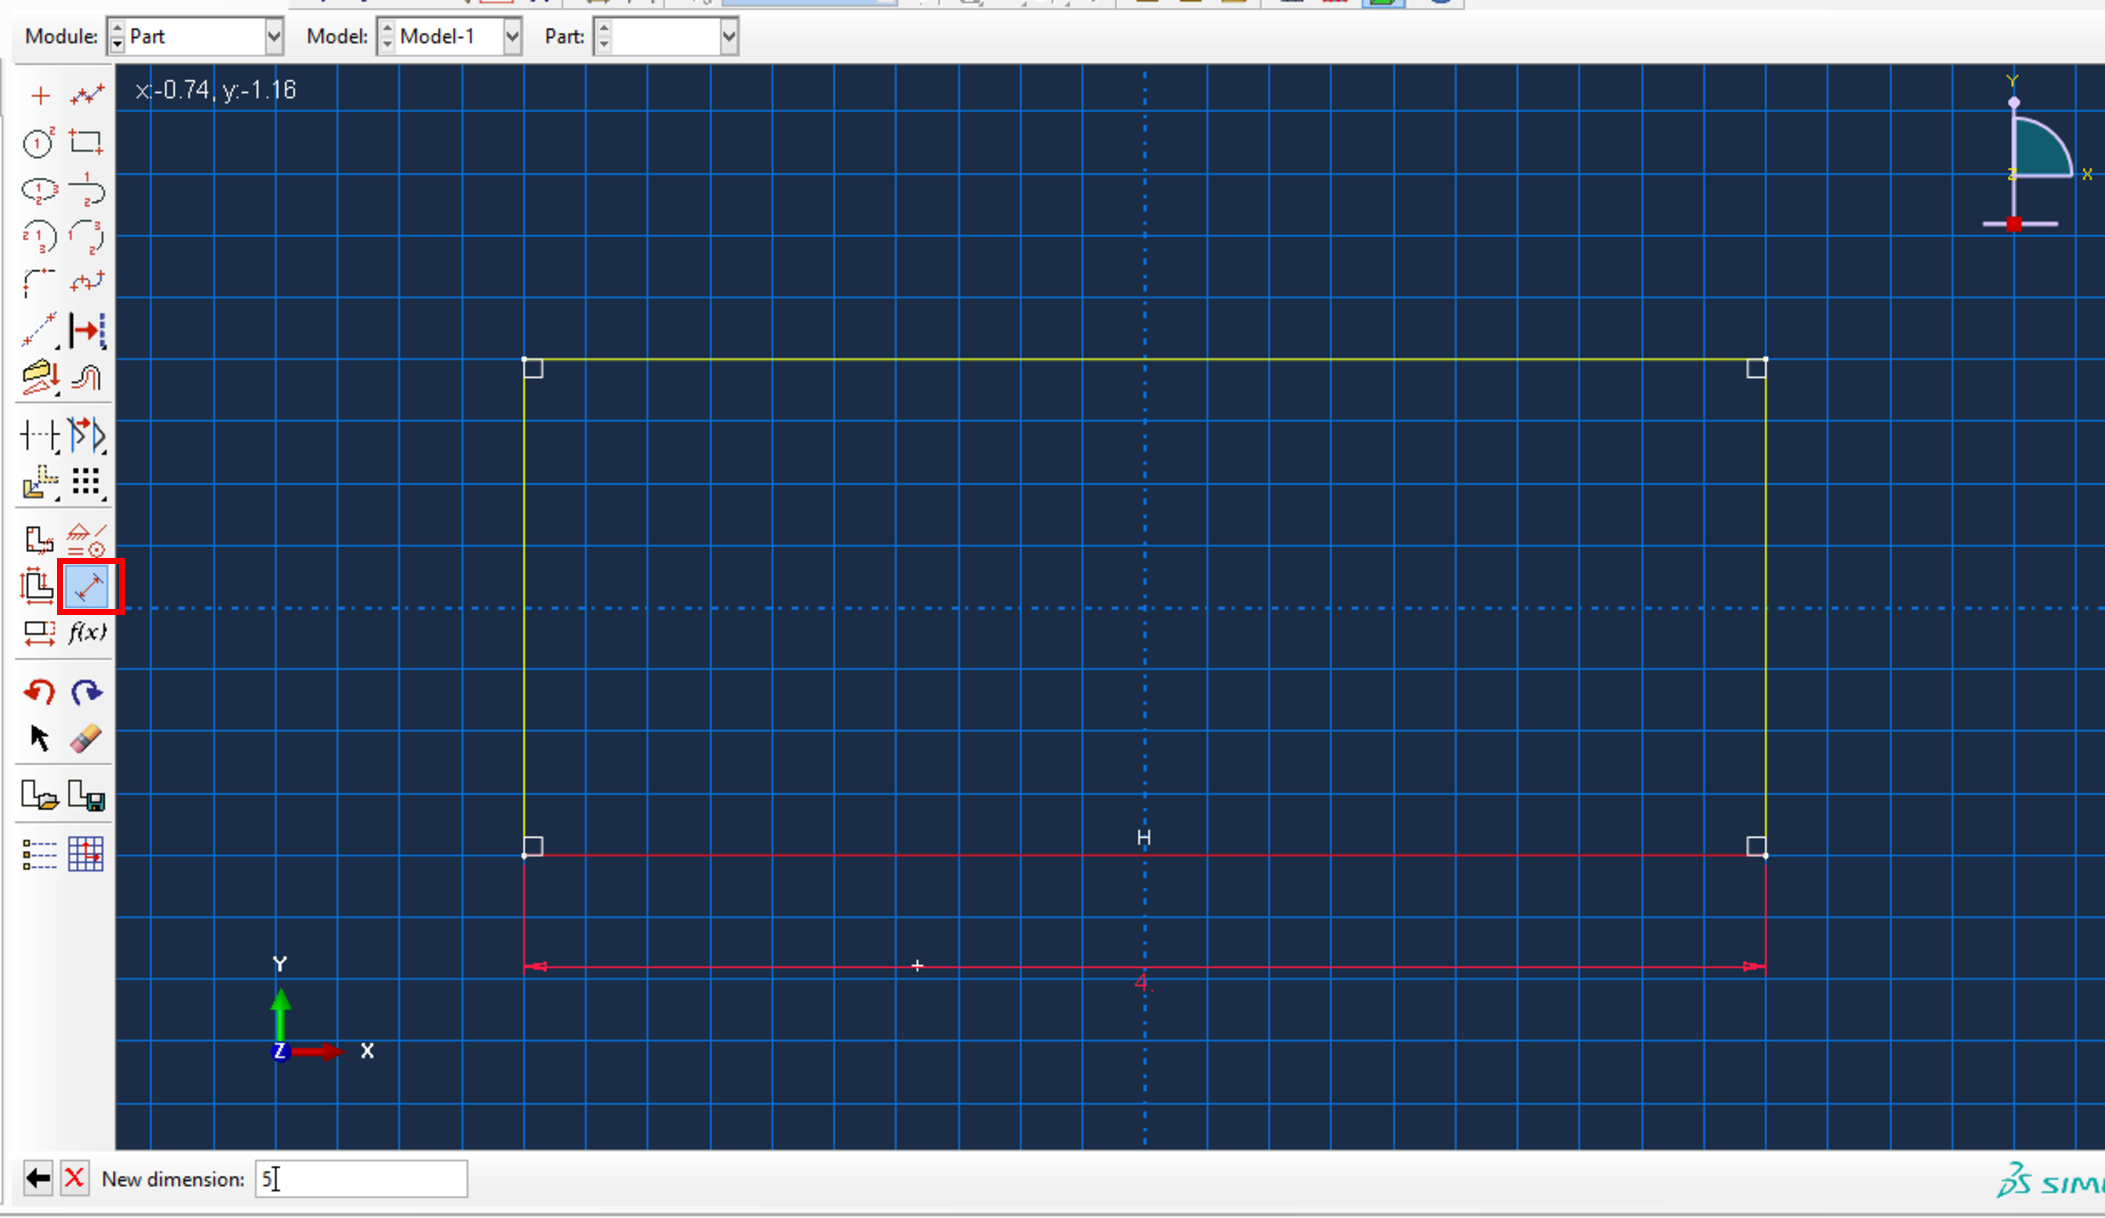
\includegraphics[width=0.875\textwidth]{./body/images/imagen06.pdf}
      \end{center}
      \caption{Modifying a Dimension}
      \label{figu06}
    \end{figure}

  \item As in the previous action modifies the vertical dimension to
    1 meter. Once done, press \textbf{Auto Fit view} to center the
    image (it should look like in Fig.~\ref{figu07}).
    \begin{figure}[!h]
      \begin{center}
        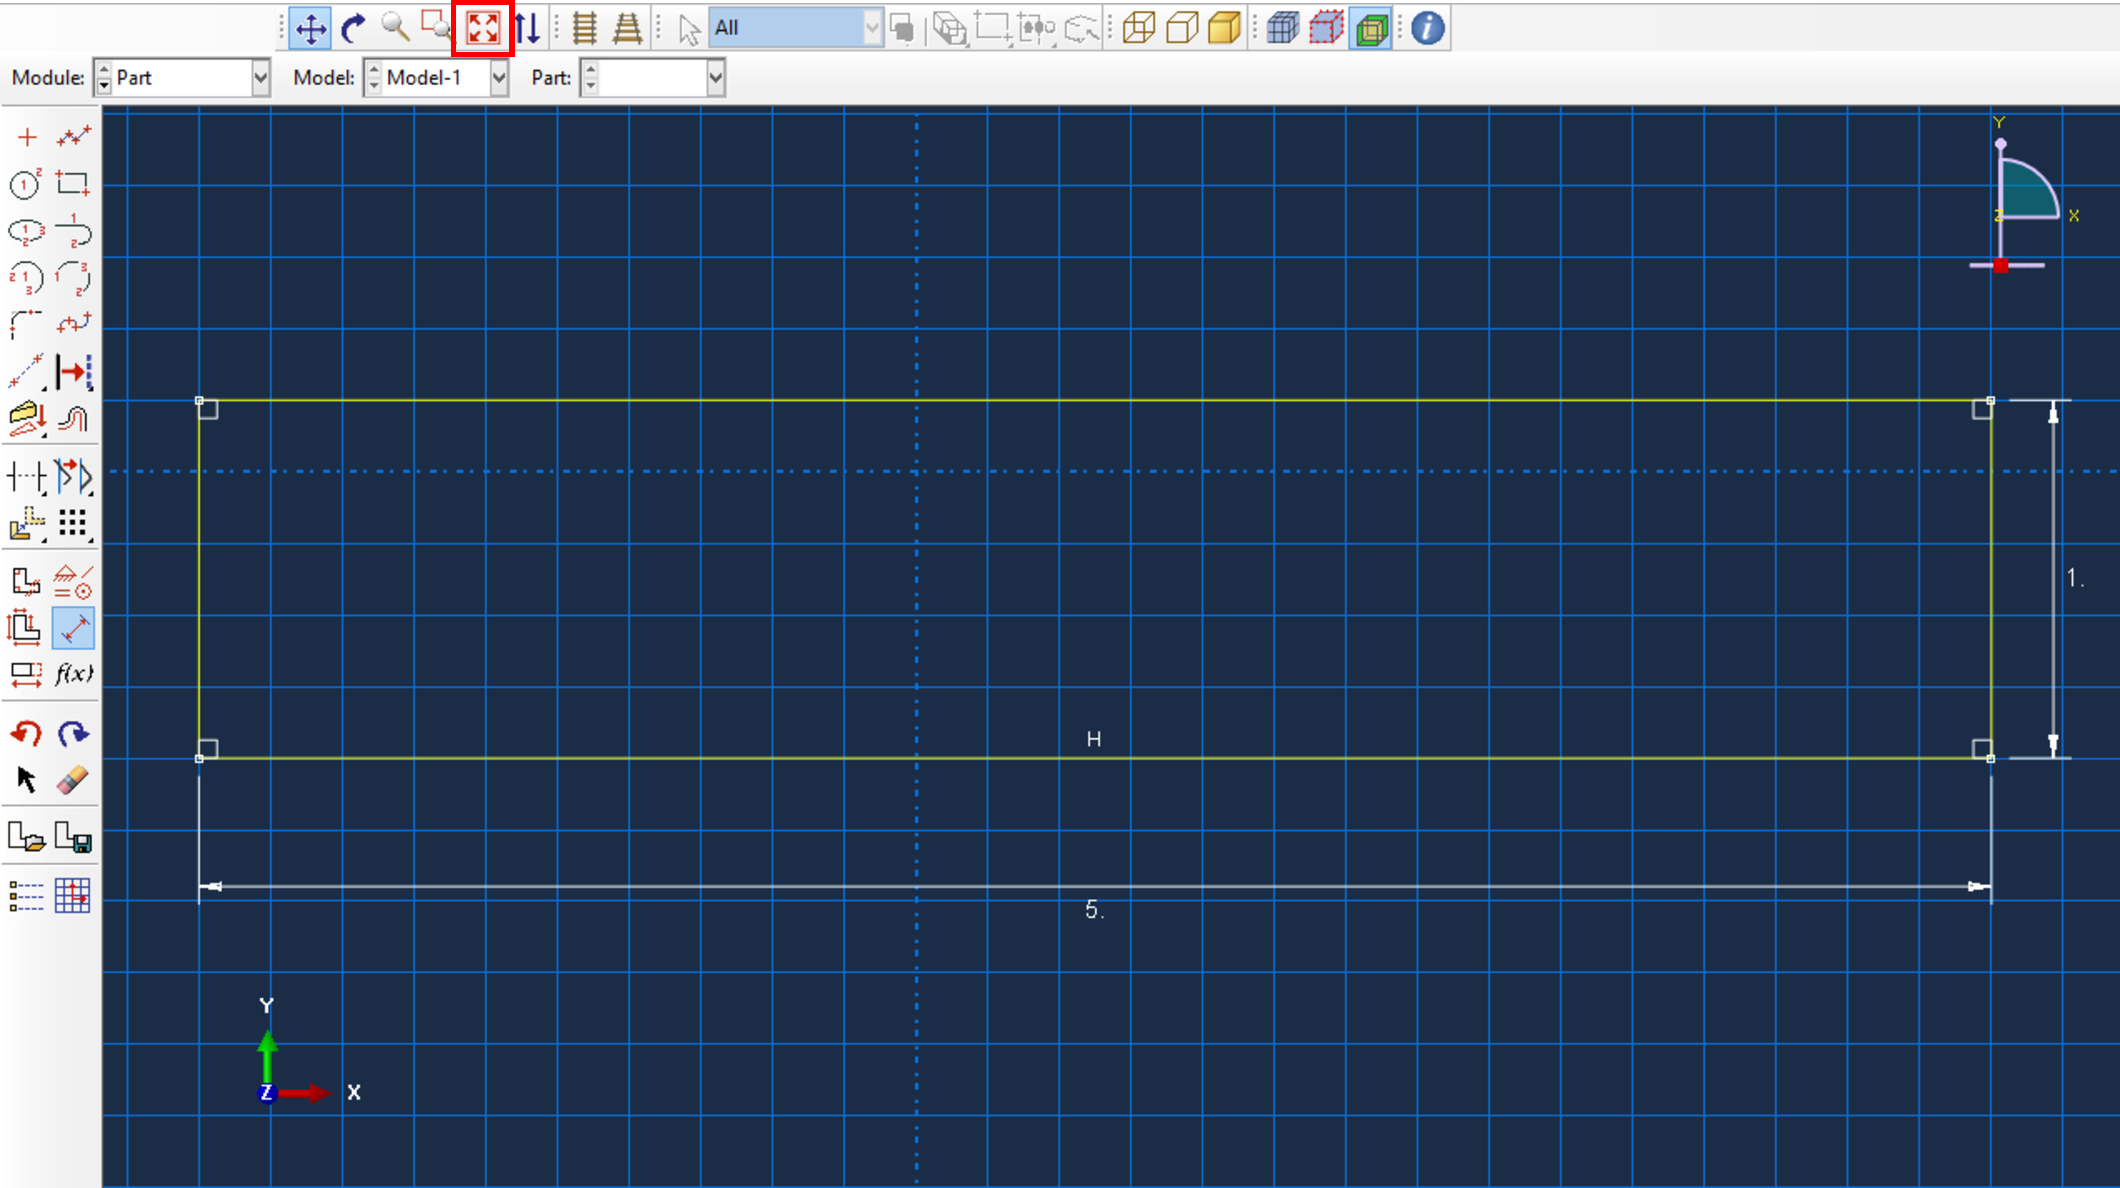
\includegraphics[width=0.875\textwidth]{./body/images/imagen07.pdf}
      \end{center}
      \caption{Final Rectangle}
      \label{figu07}
    \end{figure}

  \item Finally, press cancel to quit the Sketcher tool and press
    \textbf{Done} to generate the \textit {part} that we were looking
    for (see Fig.~\ref{figu08}).
    \begin{figure}[!h]
      \begin{center}
        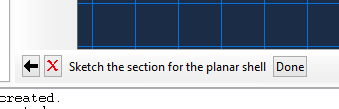
\includegraphics[width=0.55\textwidth]{./body/images/imagen08}
      \end{center}
      \caption{Final order to create object \textit{Part}}
      \label{figu08}
    \end{figure}
  \end{enumerate}


\item If we look at the distributed loads of our model, we must divide
  the upper edge into two halves in order to assign the loads only in
  the right upper half as indicated in Fig.~\ref{figu114}. To do so, follow
  these steps:
  \begin{enumerate}
  \item Among the icons associated with modifying a \textit{part},
    press \textbf{Partition Edge: Enter Parameter} as shown in
    Fig.~\ref {figu34}. Then select the upper edge of the beam
    (Fig.~\ref{figu35}).
    \begin{figure}[H]
      \centering
      \begin{subfigure}{0.29\textwidth}
        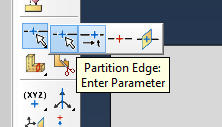
\includegraphics[width=\textwidth]{./body/images/imagen34}
        \caption{Activation of \textbf{Partition Edge}}
        \label{figu34}
      \end{subfigure}%
      ~ %add desired spacing between images, e. g. ~, \quad, \qquad, \hfill etc.
      % (or a blank line to force the subfigure onto a new line)
      \begin{subfigure}{0.59\textwidth}
        
\includegraphics[width=\textwidth]{./body/images/imagen35}
        \caption{Selection of upper edge}
        \label{figu35}
      \end{subfigure}%
      \caption{Split of upper edge}
    \end{figure}
  \item Then it asks for a parameter between 0 and 1 to indicate the
    cut-off point according to the direction of the vector that is
    seen on the screen. Since we want to divide by half, indicate 0.5
    as indicated in Fig.~\ref{figu36}.
    \begin{figure}[!h]
      \begin{center}
        
\includegraphics[width=0.75\textwidth]{./body/images/imagen36}
      \end{center}
      \caption{Introduction of split parameter}
      \label{figu36}
    \end{figure}
  \end{enumerate}
\end{enumerate}
Once the \textit{Part} is created, save the model with the
\textbf{Save model database} command.

\newpage
\subsection{Module Property. Define materials and sections.}

In this module we must define the materials, the sections and assign
this information to the \textit{part} we created in the previous
section.

\begin{enumerate}
\item \textbf{Define the material.} We choose the \textbf{Property}
  module and click on the \textbf{Create Material} icon (see
  Fig.~\ref{figu13}). In the window that appears to define the
  material we give a name, include a brief description and assign the
  constitutive mechanical behavior \textbf{Elastic} as summarized in
  Fig.~\ref{figu14}. Finally we assign the mechanical properties of a
  standard concrete ($ E = 27$ GPa , $ \nu = 0.3 $) as shown in
  Fig.~\ref{figu15}.

\begin{figure}[H]
  \centering
  \begin{subfigure}{0.19\textwidth}
    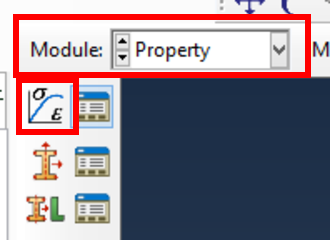
\includegraphics[width=\textwidth]{./body/images/imagen13.pdf}
    \caption{Command \textbf{Create Material}}
    \label{figu13}
  \end{subfigure}%
  ~ %add desired spacing between images, e. g. ~, \quad, \qquad, \hfill etc.
  % (or a blank line to force the subfigure onto a new line)
  \begin{subfigure}{0.39\textwidth}
    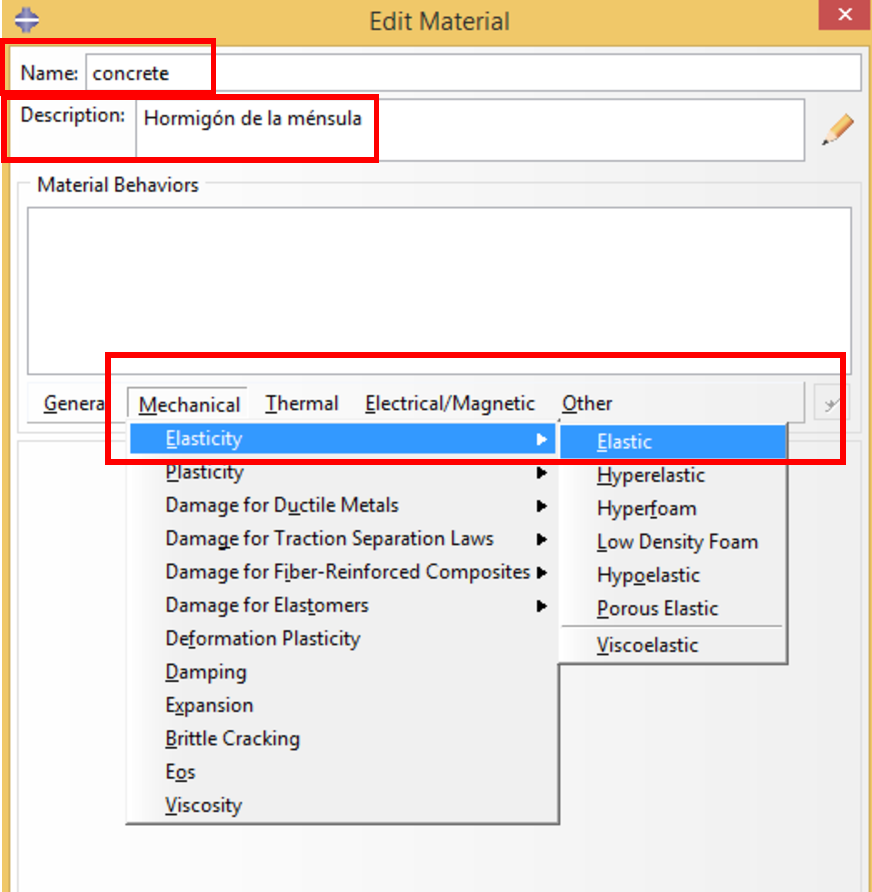
\includegraphics[width=\textwidth]{./body/images/imagen14.pdf}
    \caption{Select type of behavior}
    \label{figu14}
  \end{subfigure}
  ~ %add desired spacing between images, e. g. ~, \quad, \qquad, \hfill etc.
  % (or a blank line to force the subfigure onto a new line)
  \begin{subfigure}{0.39\textwidth}
    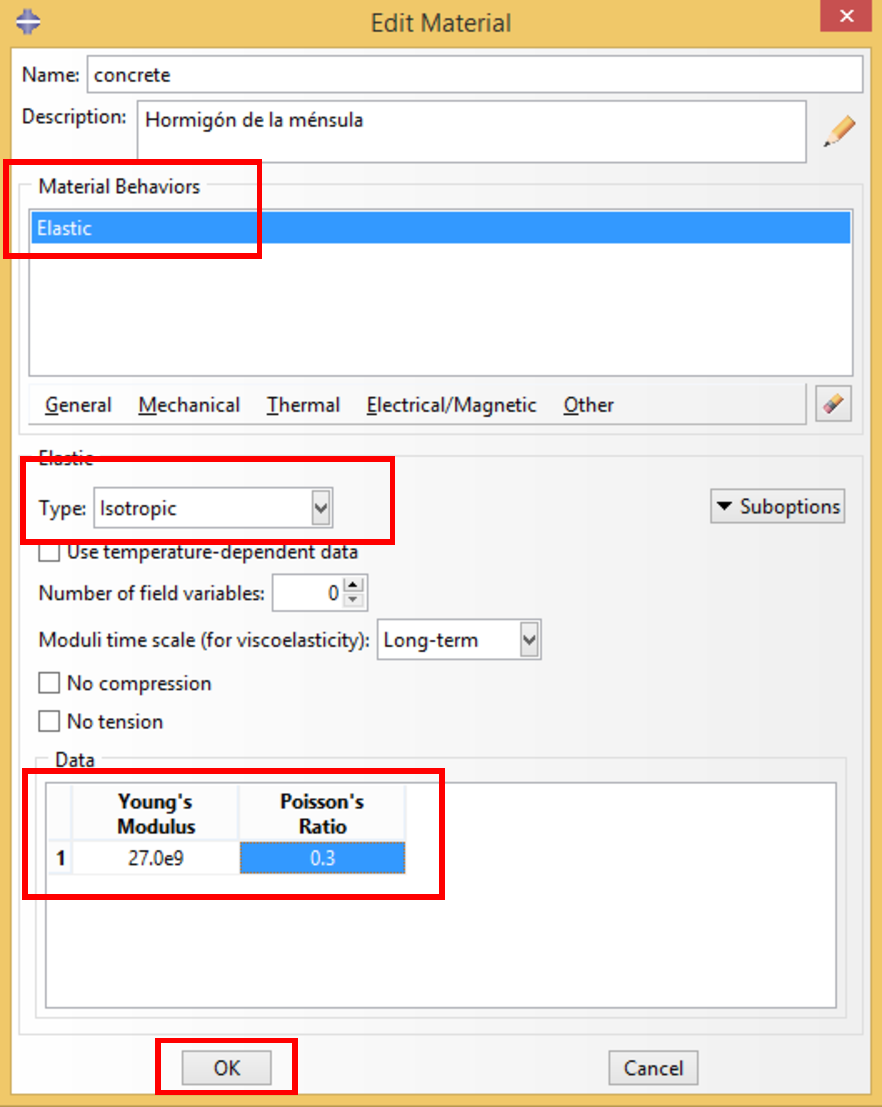
\includegraphics[width=\textwidth]{./body/images/imagen15.pdf}
    \caption{Definition of material parameters}
    \label{figu15}
  \end{subfigure}
  ~ %add desired spacing between images, e. g. ~, \quad, \qquad, \hfill etc.
  % (or a blank line to force the subfigure onto a new line)
  \caption{Definition of \textit{concrete} material}
\end{figure}

\item \textbf{Define the section.} Still within the \textbf {Property}
  module click on the \textbf{Create Section} icon (see
  Fig.~\ref{figu16}). In the next window (Fig.~\ref{figu17}) let's
  assign the name \textit{sectionMensula}, the category of finite
  element \textbf{Solid} and the type \textbf{Homogeneous}. Finally we
  associate this section with the concrete material as indicated in
  Fig.~\ref{figu18} (note that the default thickness of the piece is 1
  meter, which matches our dimension).
  \begin{figure}[H]
    \centering
    \begin{subfigure}{0.19\textwidth}
      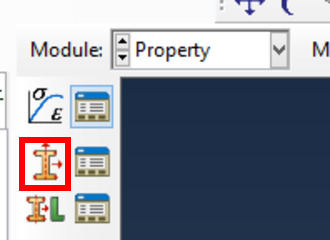
\includegraphics[width=\textwidth]{./body/images/imagen16.pdf}
      \caption{Command \textbf{Create Section}}
      \label{figu16}
    \end{subfigure}%
    ~ %add desired spacing between images, e. g. ~, \quad, \qquad, \hfill etc.
    % (or a blank line to force the subfigure onto a new line)
    \begin{subfigure}{0.39\textwidth}
      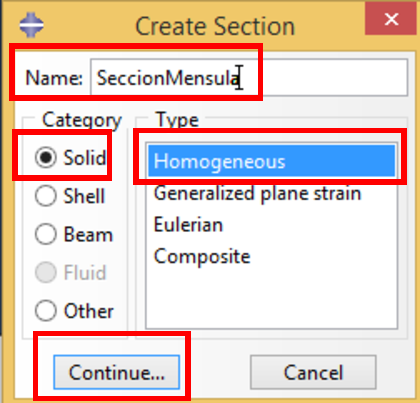
\includegraphics[width=\textwidth]{./body/images/imagen17.pdf}
      \caption{Definition of section properties}
      \label{figu17}
    \end{subfigure}
    ~ %add desired spacing between images, e. g. ~, \quad, \qquad, \hfill etc.
    % (or a blank line to force the subfigure onto a new line)
    \begin{subfigure}{0.39\textwidth}
      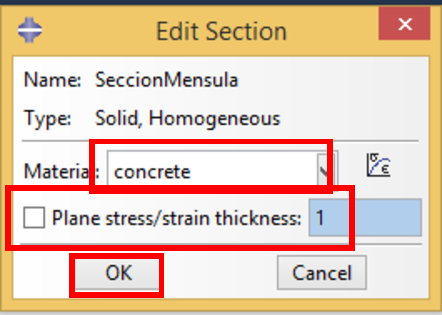
\includegraphics[width=\textwidth]{./body/images/imagen18.pdf}
      \caption{Association of the material to the section}
      \label{figu18}
    \end{subfigure}
    ~ %add desired spacing between images, e. g. ~, \quad, \qquad, \hfill etc.
    % (or a blank line to force the subfigure onto a new line)
    \caption{Definition of section \textit{SeccionMensula}}
  \end{figure}


\item \textbf{Assign the section to a part.}  Finally, in this module
  we must assign the previous section to the created \textit{part}. To
  do so, click on the icon \textbf{Assign Section} (see
  Fig.~\ref{figu21}) and select the region to which we want to assign
  the section (the beam). We choose  we want to assign the section
  \textit{SeccionMesula} (see Fig.~\ref{figu19}) and our \textit{part}
  should have changed color as indicated in Fig.~\ref{figu20}
  \begin{figure}[H]
    \centering
    \begin{subfigure}{0.19\textwidth}
      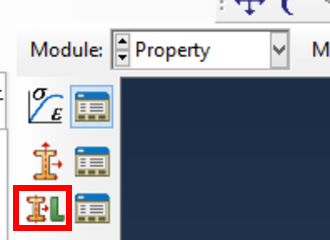
\includegraphics[width=\textwidth]{./body/images/imagen21.pdf}
      \caption{Command \textbf{Assign Section}}
      \label{figu21}
    \end{subfigure}%
    ~ %add desired spacing between images, e. g. ~, \quad, \qquad, \hfill etc.
    % (or a blank line to force the subfigure onto a new line)
    \begin{subfigure}{0.29\textwidth}
      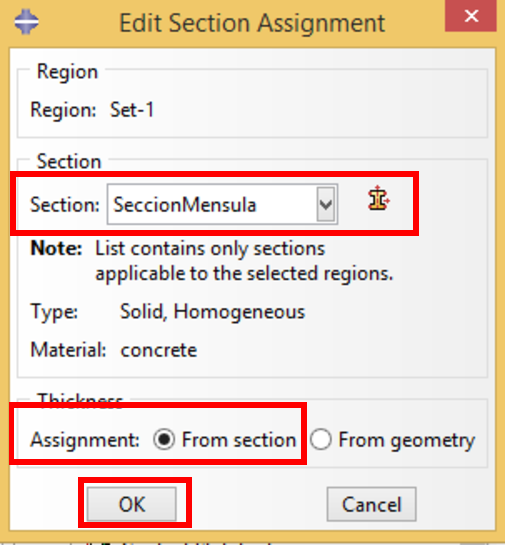
\includegraphics[width=\textwidth]{./body/images/imagen19.pdf}
      \caption{Association of the section to the Part}
      \label{figu19}
    \end{subfigure}%
    ~ %add desired spacing between images, e. g. ~, \quad, \qquad, \hfill etc.
    % (or a blank line to force the subfigure onto a new line)
    \begin{subfigure}{0.49\textwidth}
      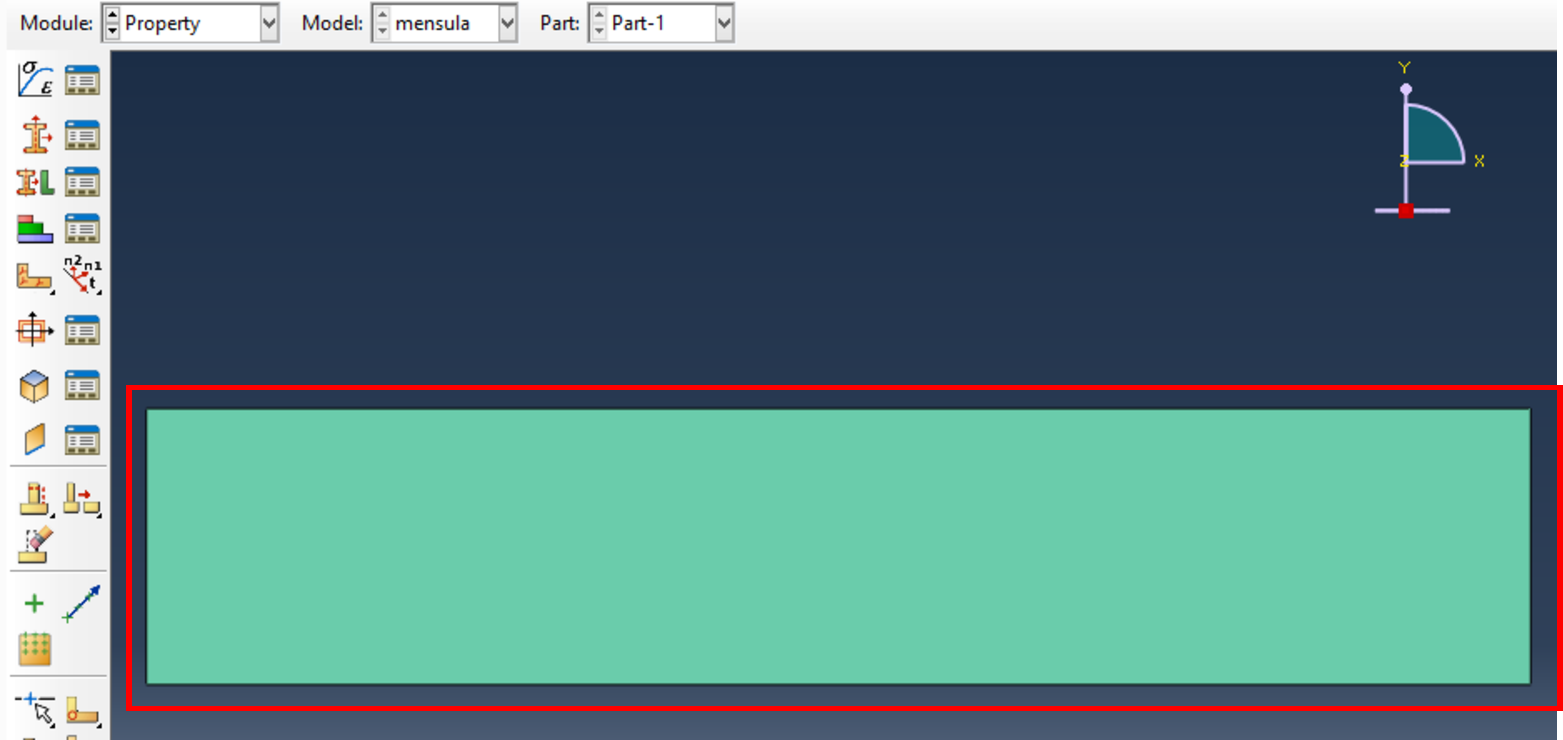
\includegraphics[width=\textwidth]{./body/images/imagen20.pdf}
      \caption{Part with assigned section}
       \label{figu20}
    \end{subfigure}
    \caption{Assigning the section to a \textit{Part}}
  \end{figure}
\end{enumerate}
\newpage
\subsection{Module Assembly. Assemble the model}
Every Abaqus model is constructed as a set of copies
(\textit{instances}) of the created \textit{parts}. Our problem is
very simple and we just have to create a set (\textit{Assembly}) with
a single copy of our \textit {part}. However, imagine that we would
like to model a car, and that we have created \textit{parts} of its
different components. With Abaqus's logic we would have created a
\textit{part} defining a wheel, and at the time of assembling the
final model, we would make four copies of that \textit{part} (one for
each wheel of the car).


In order to assembly our model follow the next steps:
\begin{enumerate}
\item Activate the module \textbf{Assembly} and press the
  \textbf{Create instance} icon as shown in Fig.~\ref{figu22}.
\item In the dialog box that appears (see Fig.~\ref{figu23}), select
  the \textit{part} we are going to make a copy of (there is only one
  in our problem) and indicates that the copy will be of type
  \textbf{Dependent} (we will define the mesh in the \textit {part}
  and it will be replicated in the copy we are creating).
\end{enumerate}

\begin{figure}[H]
  \centering
  \begin{subfigure}{0.25\textwidth}
    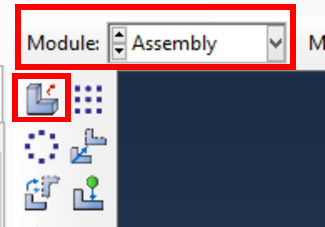
\includegraphics[width=\textwidth]{./body/images/imagen22.pdf}
    \caption{Command \textbf{Create instance}}
    \label{figu22}
  \end{subfigure}%
  ~ %add desired spacing between images, e. g. ~, \quad, \qquad, \hfill etc.
  % (or a blank line to force the subfigure onto a new line)
  \begin{subfigure}{0.42\textwidth}
    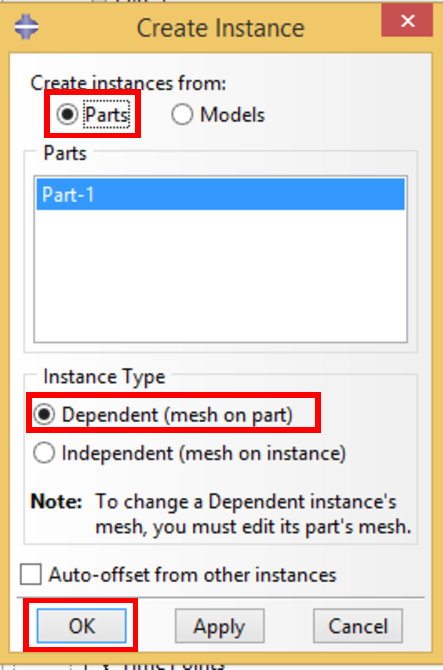
\includegraphics[width=\textwidth]{./body/images/imagen23.pdf}
    \caption{Creating a \textit{Dependent} copy}
    \label{figu23}
  \end{subfigure}%
  \caption{Action \textbf{Create Instance}}
\end{figure}

In order to facilitate later operations, Abaqus allows us to group nodal points
of geometric entities into objects called \textbf{sets}. In this way,
when we want to obtain the results in that geometric entity we can
request it to Abaqus without needing to know the nodes of the mesh
that form it (only the name of the \textbf{set}). In our case we want
to know the distribution of the nodal forces in the clamped end of the
beam. So we are going to create a set of the future mesh nodes in this
geometry:
\begin{enumerate}
\item To create a set, double-click on the \textbf{Sets} element in the \textbf{Model Tree} (see Fig.~\ref{figu24}) or press \textbf{Tools/Set/Create} (see Fig.~\ref{figu25}).
  \begin{figure}[H]
    \centering
    \begin{subfigure}{0.35\textwidth}
      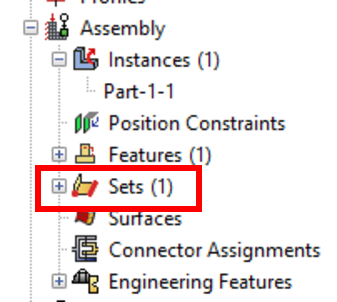
\includegraphics[width=\textwidth]{./body/images/imagen24.pdf}
      \caption{\textbf{Model Tree}}
      \label{figu24}
    \end{subfigure}%
    ~ %add desired spacing between images, e. g. ~, \quad, \qquad, \hfill etc.
    % (or a blank line to force the subfigure onto a new line)
    \begin{subfigure}{0.40\textwidth}
      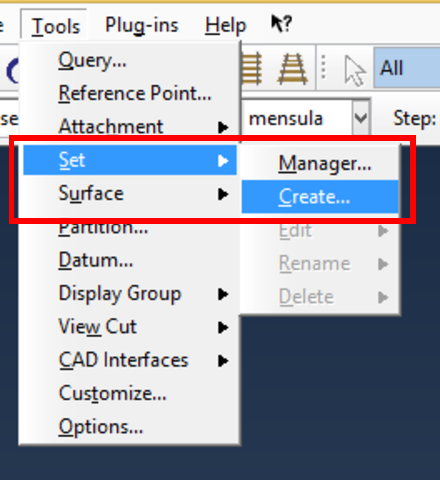
\includegraphics[width=\textwidth]{./body/images/imagen25.pdf}
      \caption{Start creation \textbf{set}}
      \label{figu25}
    \end{subfigure}%
    \caption{Creation of a \textbf{set}}
  \end{figure}
\item Set the name \textit{LadoIzquierdo} in next window (see Fig.~\ref{figu26}) and select the left side of the beam (see Fig.~\ref{figu27}). 
  \begin{figure}[H]
    \centering
    \begin{subfigure}{0.25\textwidth}
      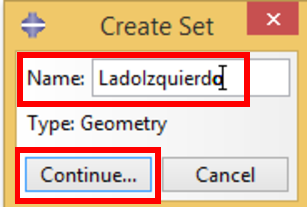
\includegraphics[width=\textwidth]{./body/images/imagen26.pdf}
      \caption{Assignment of the set name}
      \label{figu26}
    \end{subfigure}%
    ~ %add desired spacing between images, e. g. ~, \quad, \qquad, \hfill etc.
    % (or a blank line to force the subfigure onto a new line)
    \begin{subfigure}{0.28\textwidth}
      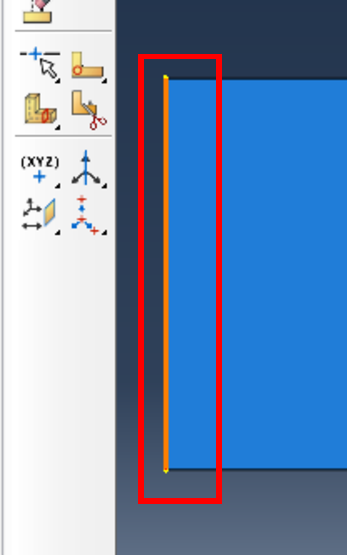
\includegraphics[width=\textwidth]{./body/images/imagen27.pdf}
      \caption{Selection of the left side}
      \label{figu27}
    \end{subfigure}%
    \caption{Creation of a \textbf{set}}
  \end{figure}
\item Make sure that in the Model Tree a new set has been created (as shown in Fig.~\ref{figu28})
  \begin{figure}
    \centering
    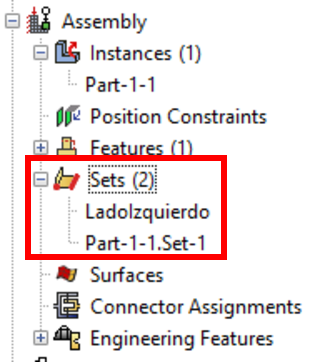
\includegraphics[width=0.39\textwidth]{./body/images/imagen28.pdf}
    \caption{\textbf{Model Tree} with two sets}
    \label{figu28}
  \end{figure}
\end{enumerate}
\newpage
\subsection{Module Step. Configure the analysis procedure.}

Once the model is built, we must define in Abaqus the calculation
steps (\textbf{steps}) that we will use in our analysis and what
information we want to keep from each one. Abaqus defines a
calculation step \textit{Initial} that we will assume is the beginning
of our analysis (everything that happens before our analysis) where, in our case, we
will apply the boundary condition in displacements (the encastre) at
the left side of the beam. After that, to apply the imposed tension
vector, we will define a single calculation step and perform a static
analysis. To define the calculation step (\textbf {Step}) do as
follows:
\begin{enumerate}
\item Activate the \textbf{Step} module and click on the
  \textbf{Create Steps} icon as shown in Fig.~\ref{figu29}. In the
  dialog box that appears (see Fig.~\ref{figu30}) name the case as
  \textit{Static Case} and indicates that the analysis is of
  \textbf{Static, General} type. Set everything else as default.
  \begin{figure}[H]
    \centering
    \begin{subfigure}{0.29\textwidth}
      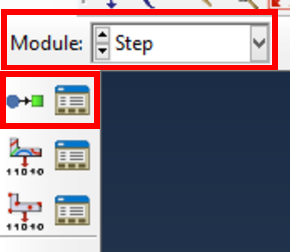
\includegraphics[width=\textwidth]{./body/images/imagen29.pdf}
      \caption{Command \textbf{Create Steps}}
      \label{figu29}
    \end{subfigure}%
    ~ %add desired spacing between images, e. g. ~, \quad, \qquad, \hfill etc.
    % (or a blank line to force the subfigure onto a new line)
    \begin{subfigure}{0.40\textwidth}
      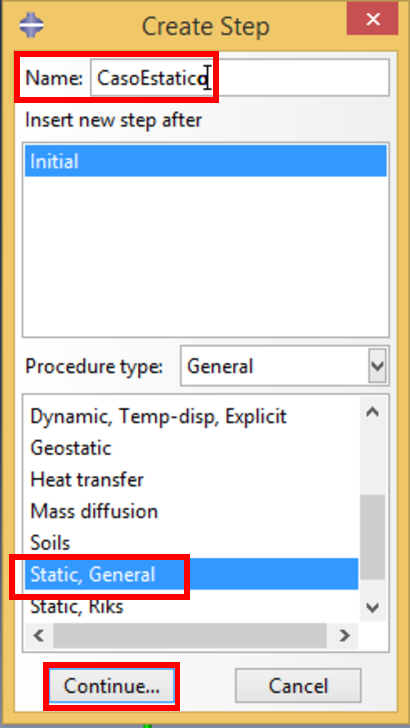
\includegraphics[width=\textwidth]{./body/images/imagen30.pdf}
      \caption{Properties of the new calculation step}
      \label{figu30}
    \end{subfigure}%
    \caption{Create new calculation step}
  \end{figure}
\item Now let's decide what information we want to keep from the
  calculation step created to be able to analyze it afterwards it in the
  postprocess. Under the name \textbf{Field Output} Abaqus stores
  solution information in the space domain at a given time. Select the
  \textbf{Create Field Output} icon (see Fig.~\ref{figu31}) to create
  a new result field. In the following dialog name it
  \textit{F-Output-New} and assign it to the interval just created
  \textit{CasoEstatico} (see Fig.~\ref{figu32}). From the fields
  available for postprocessing, we will choose the stress tensor (S),
  the von Mises equivalent stress (MISES), the displacements (U), the
  reaction forces and moments (RF) and the forces and moments
  concentrated (CF) as indicated in Fig.~\ref{figu33}.
  \begin{figure}[H]
    \centering
    \begin{subfigure}{0.25\textwidth}
      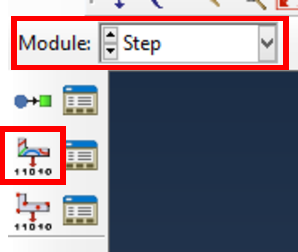
\includegraphics[width=\textwidth]{./body/images/imagen31.pdf}
      \caption{Create new \textbf{Field Output}}
      \label{figu31}
    \end{subfigure}%
    ~ %add desired spacing between images, e. g. ~, \quad, \qquad, \hfill etc.
    % (or a blank line to force the subfigure onto a new line)
    \begin{subfigure}{0.33\textwidth}
      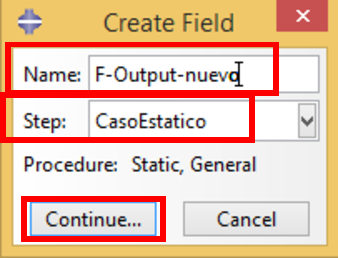
\includegraphics[width=\textwidth]{./body/images/imagen32.pdf}
      \caption{Associate \textbf{Field Output} to the
        \textbf{Step}}
      \label{figu32}
    \end{subfigure}%
    ~ %add desired spacing between images, e. g. ~, \quad, \qquad, \hfill etc.
    % (or a blank line to force the subfigure onto a new line)
    \begin{subfigure}{0.40\textwidth}
      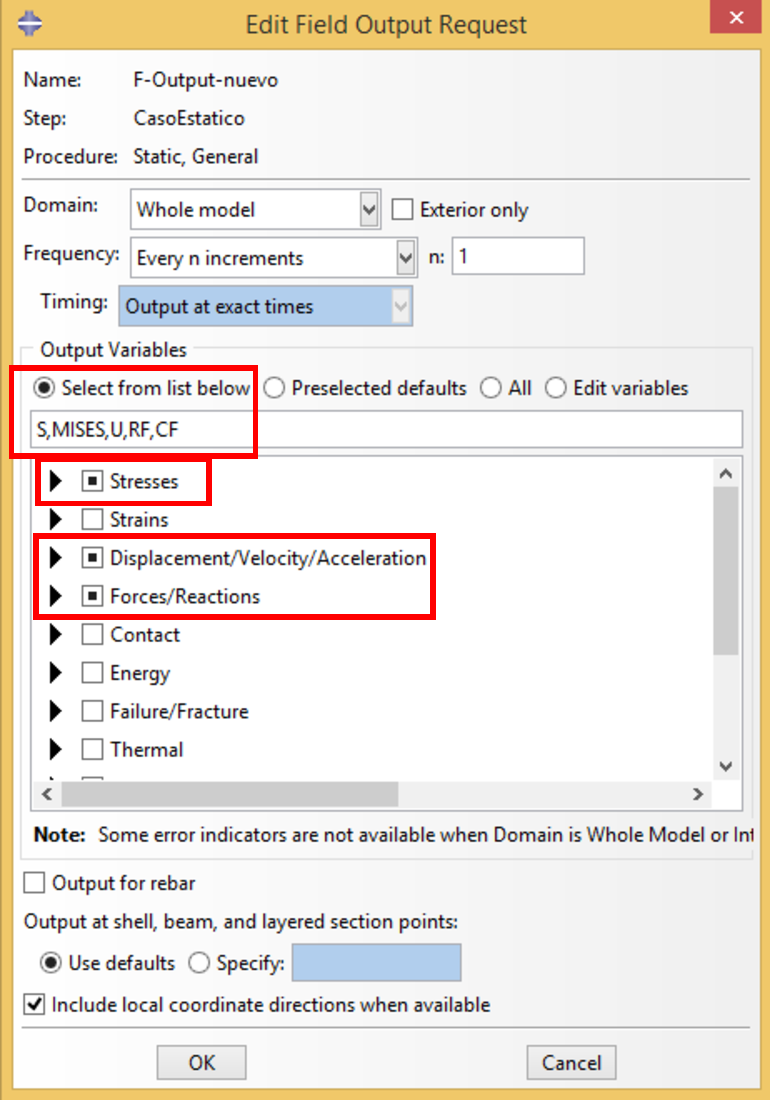
\includegraphics[width=\textwidth]{./body/images/imagen33.pdf}
      \caption{Definition of the \textbf{Field Output} components}
      \label{figu33}
    \end{subfigure}%
    \caption{\textbf{Field Output} definition}
  \end{figure}
\item Under the name \textbf{History Output} Abaqus stores the
  solution information at a spatial point during a time interval. Since we are
  in a quasi-static problem we are not interested in the temporal
  evolution of a variable and we are going to eliminate the one that
  Abaqus creates by default. To do so press the right mouse button on
  the \textbf{History Output Request} node of the \textbf{Model
    Tree} and select \textbf{Manager} as indicated in
  Fig.~\ref{figu41}. We will see a window with the historical variable
  manager (see Fig.~\ref{figu42}), select the variable
  \textbf{H-Output-1} and press \textbf{Delete}.

  \begin{figure}[H]
    \centering
    \begin{subfigure}{0.45\textwidth}
      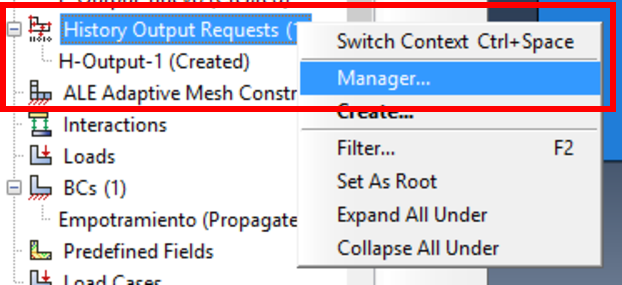
\includegraphics[width=\textwidth]{./body/images/imagen41.pdf}
      \caption{Opening \textbf{History Outputs} manager}
      \label{figu41}
    \end{subfigure}%
    ~ %add desired spacing between images, e. g. ~, \quad, \qquad, \hfill etc.
    % (or a blank line to force the subfigure onto a new line)
    \begin{subfigure}{0.45\textwidth}
      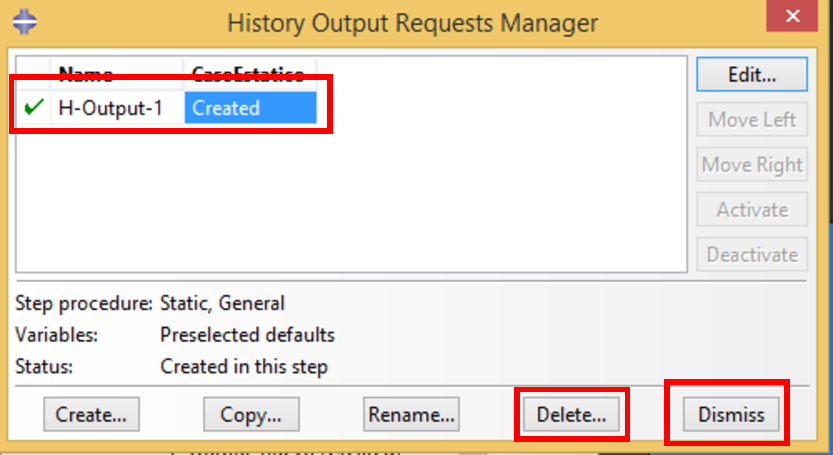
\includegraphics[width=\textwidth]{./body/images/imagen42.pdf}
      \caption{\textbf{History Outputs} manager}
      \label{figu42}
    \end{subfigure}%
    \caption{Delete of \textbf{History Outputs}}
  \end{figure}
\end{enumerate}
\newpage
\subsection{Module Load. Apply the boundary conditions}

We want to apply essential boundary conditions (we
impose null displacement in the encastre) and  natural boundary conditions (we
impose a tension vector $ \textbf{t}^*$ in the right half of the  upper
part of the beam).  The encastre will be applied in the calculation
step \textit{Initial} and the tension vector in the calculation step
\textit{CasoEstatico} previously created.

In order to impose the essential boundary condition do as
follows:
\begin{enumerate}
\item Activate the \textbf{Load} module and press \textbf{Create
    Boundary Condition} (see Fig.\ref{figu37}).
  \begin{figure}[!h]
    \centering
    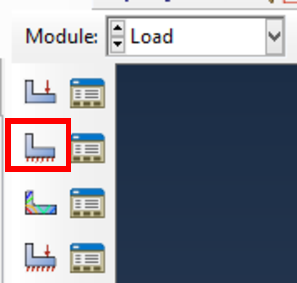
\includegraphics[width=0.33\textwidth]{./body/images/imagen37.pdf}
    \caption{Command \textbf{Create Boundary Condition}}
    \label{figu37}
  \end{figure}
\item In the dialog box that appears (see Fig.\ref{figu38}), put the
  name \textit{Empotramiento} to the boundary condition, assign it to the
  calculation step \textbf{Initial}, set the category
  \textbf{Mechanical} and the type
  \textbf{Symmetry/Antisymmetry/Encastre}. Select the left side where
  we will impose the boundary condition. In the following dialog box set
   the boundary condition is of \textbf{Encastre} (clamped) type
  as indicated in Fig.~\ref{figu39}.
  \begin{figure}[H]
    \centering
    \begin{subfigure}{0.45\textwidth}
      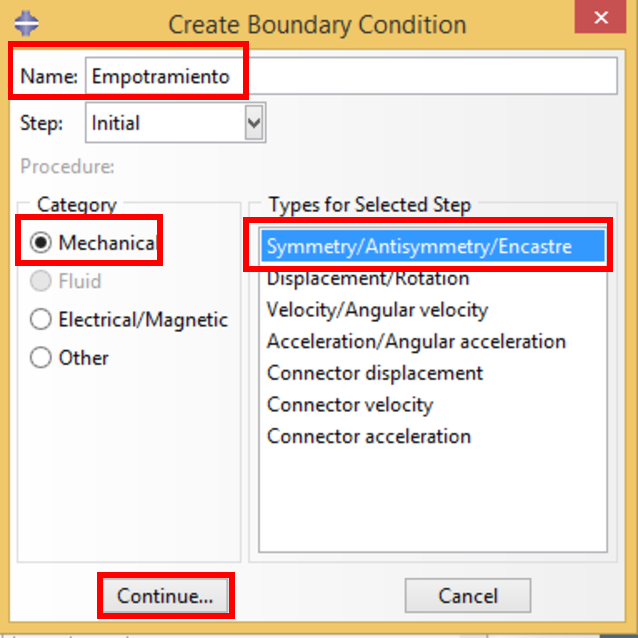
\includegraphics[width=\textwidth]{./body/images/imagen38.pdf}
      \caption{Creating of boundary condition}
      \label{figu38}
    \end{subfigure}%
    ~ %add desired spacing between images, e. g. ~, \quad, \qquad, \hfill etc.
    % (or a blank line to force the subfigure onto a new line)
    \begin{subfigure}{0.45\textwidth}
      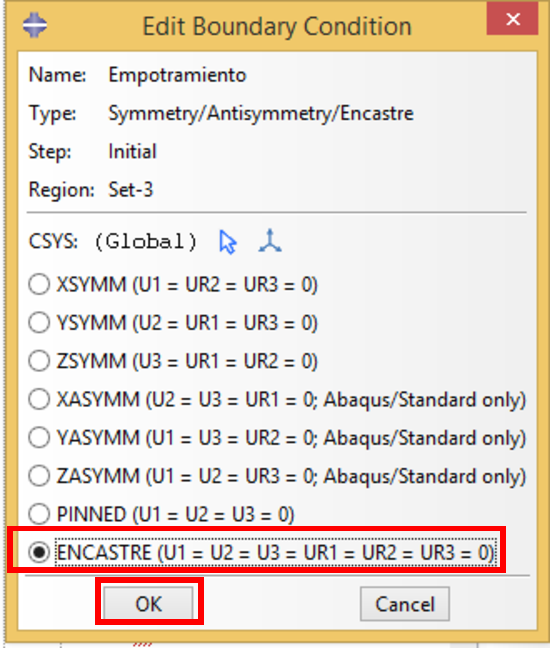
\includegraphics[width=\textwidth]{./body/images/imagen39.pdf}
      \caption{Editing of boundary condition}
      \label{figu39}
    \end{subfigure}%
    \caption{Definition of boundary condition \textit{encastre}}
  \end{figure}
\item Finally, the model we have created has to appear on the working
  screen with the degrees of freedom on the left side of the beam set
  to zero (see Fig.\ref{figu40})
  \begin{figure}
    \centering
    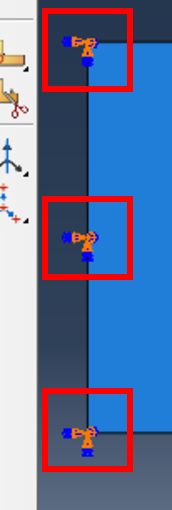
\includegraphics[width=0.19\textwidth]{./body/images/imagen40.pdf}
    \caption{Detail of the encastre boundary condition}
    \label{figu40}
  \end{figure}
\end{enumerate}


In order to impose the natural boundary condition do as follows:
\begin{enumerate}
\item Press the \textbf{Create Load} icon as shown in
  Fig.~\ref{figu43}. In the dialog box that appears (see
  Fig.~\ref{figu44}) name the boundary condition as
  \textit{CargaRepartida}, apply it in the calculation step
  \textit{CasoEstatico}, indicating that its category is
  \textbf{Mechanical} and the type \textbf{Surface traction}. Select
  the right half of the upper edge of the beam as described in
  Fig.~\ref{figu45}.
  \begin{figure}[H]
    \centering
    \begin{subfigure}{0.23\textwidth}
      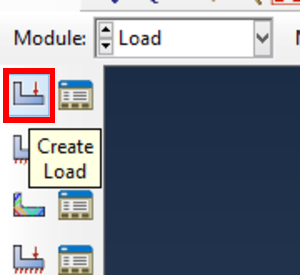
\includegraphics[width=\textwidth]{./body/images/imagen43.pdf}
      \caption{Command \textbf{Create Load}}
      \label{figu43}
    \end{subfigure}%
    ~ %add desired spacing between images, e. g. ~, \quad, \qquad, \hfill etc.
    % (or a blank line to force the subfigure onto a new line)
    \begin{subfigure}{0.30\textwidth}
      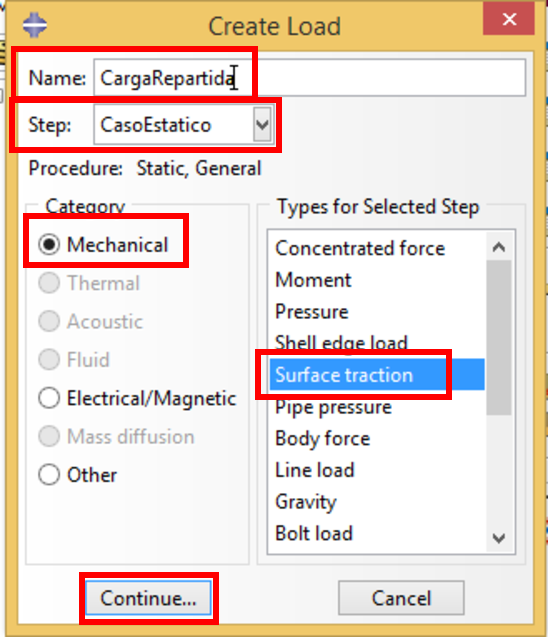
\includegraphics[width=\textwidth]{./body/images/imagen44.pdf}
      \caption{Type of load}
      \label{figu44}
    \end{subfigure}%
    ~ %add desired spacing between images, e. g. ~, \quad, \qquad, \hfill etc.
    % (or a blank line to force the subfigure onto a new line)
    \begin{subfigure}{0.44\textwidth}
      \includegraphics[width=\textwidth]{./body/images/imagen45.pdf}
      \caption{Selection of upper left edge}
      \label{figu45}
    \end{subfigure}%
    \caption{Definition of distributed load (I)}
  \end{figure}
\item The following dialog box allows us to define the tension
  vector. Set the type as \textbf{General} and a module of value 1000
  Pa (see Fig.~\ref{figu46}). It is necessary to define the direction
  and sense of the tension vector. Click on the blue arrow next to the
  word \textbf{Vector} to define a vector that gives us the direction
  and sense of the vector tension (it does not have to be unitary). It
  can be done by pressing two vertices of our geometry or by entering
  two pairs of coordinates. Let's do it the last way. Enter the
  coordinates of the starting point (Fig.~\ref{figu47}, then press
  enter) and the end point (Fig.~\ref{figu48}, then press enter).

\begin{figure}[H]
  \centering
  \begin{varwidth}{0.40\linewidth} % this is a must
    \begin{subfigure}{0.95\textwidth}
      \includegraphics[width=\textwidth]{./body/images/imagen46.pdf}
      \caption{Properties of tension vector}
      \label{figu46}
    \end{subfigure}
  \end{varwidth}\quad%\quad
  \begin{varwidth}{0.60\linewidth} % this is a must
    \begin{subfigure}{0.95\textwidth}
      \includegraphics[width=\textwidth]{./body/images/imagen47.pdf}
      \caption{Start of auxiliary vector}
      \label{figu47}
    \end{subfigure}
    \\
    \begin{subfigure}{0.95\textwidth}
      \includegraphics[width=\textwidth]{./body/images/imagen48.pdf}
      \caption{End of auxiliary vector}
      \label{figu48}
    \end{subfigure}
  \end{varwidth}
  \caption{Definition of distributed load (II)}
\end{figure}

\item We now see the normalized vector in the previous dialog box (see
  Fig.~\ref{figu49}) and, in accepting the definition, the load
  distribution scheme appears in the working window (see
  Fig.~\ref{figu50}). Check in the \textbf{Model Tree} that the
  associated definitions have been added to the boundary conditions nodes (BCs and Loads).
  \begin{figure}[H]
    \centering
    \begin{subfigure}{0.30\textwidth}
      \includegraphics[width=\textwidth]{./body/images/imagen49.pdf}
      \caption{Properties of tension vector}
      \label{figu49}
    \end{subfigure}%
    ~ %add desired spacing between images, e. g. ~, \quad, \qquad, \hfill etc.
    % (or a blank line to force the subfigure onto a new line)
    \begin{subfigure}{0.67\textwidth}
      \includegraphics[width=\textwidth]{./body/images/imagen50.pdf}
      \caption{Detail of applied load}
      \label{figu50}
    \end{subfigure}%
    \caption{Definition of distributed load (III)}
  \end{figure}
\end{enumerate}

\newpage
\subsection{Module Mesh. Build the mesh.}
In order to assign a mesh to a geometry we must inform Abaqus about:
\begin{enumerate}
\item The shape of the element (whether they are triangles or squares
  in two-dimensional problems and whether they are tetrahedral or
  hexahedral in three-dimensional problems).
\item Size of the element (either a global size for the geometry or
  by defining different sizes depending on regions).
\item The type of element (we will explain this concept in following
  classes).
\end{enumerate}

Abaqus distinguishes which type of mesh can be made according to the
geometry we have (although the user can split the \textit{parts}
manually to create more regular geometries). Each possible type of
mesh in each region is identified with a color:

\begin{description}
\item[Green] Meshes can be generated using structured methods
\item[Yellow] Meshes can be generated with the sweep method
\item[Pink] Meshes can be generated with the free method
\item[Cinnamon]Meshes can be generated with the button-up method
\item[Orange] You can not generate meshes and the geometry has to be
  divided
\end{description}

But in our case it happens that the geometry is blue. This is because we
have made a dependent copy on the \textit{part} and is the part the
one that we have to mesh (then the mesh is replicated in the
copy). Activate the \textbf{Mesh} module and change the \textit{part}
as the object to mesh as indicated in Fig.~\ref{figu51} and it will
change to pink.
\begin{figure}[!h]
  \centering
  \includegraphics[width=0.95\textwidth]{./body/images/imagen51.pdf}
  \caption{Start of Mesh module}
  \label{figu51}
\end{figure}

To define the mesh, follow these steps:
\begin{enumerate}
\item First we will define the shape of the elements. Press
  \textbf{Mesh/Controls} in the upper menu bar and the dialog box in
  Fig.~\ref{figu52} appears. Let's set that we want to use
  \textbf{quadrilaterals},  the technique is \textbf{Free} and
   the algorithm is \textbf{Advancing front}.
  \begin{figure}[!h]
    \centering
    \includegraphics[width=0.50\textwidth]{./body/images/imagen52.pdf}
    \caption{Definition of the element shape}
    \label{figu52}
  \end{figure}
\item Let us now define the size of the elements. Press the
  \textbf{Seed part} icon (see Fig.~ \ref{figu53}) to assign a global
  size to the elements of the geometry. Let us use a size of 0.2 m as
  shown in Fig.~\ref{figu54} and press the \textbf{Apply} button. We
  should see a division of the boundary of our geometry using the size
  we have indicated (see Fig.~\ref{figu55}). Finally press OK.
  \begin{figure}[H]
    \centering
    \begin{subfigure}{0.15\textwidth}
      \includegraphics[width=\textwidth]{./body/images/imagen53.pdf}
      \caption{Start of command \textbf{Seed part}}
      \label{figu53}
    \end{subfigure}%
    ~ %add desired spacing between images, e. g. ~, \quad, \qquad, \hfill etc.
    % (or a blank line to force the subfigure onto a new line)
    \begin{subfigure}{0.33\textwidth}
      \includegraphics[width=\textwidth]{./body/images/imagen54.pdf}
      \caption{Global element size assignment}
      \label{figu54}
    \end{subfigure}%
    ~ %add desired spacing between images, e. g. ~, \quad, \qquad, \hfill etc.
    % (or a blank line to force the subfigure onto a new line)
    \begin{subfigure}{0.49\textwidth}
      \includegraphics[width=\textwidth]{./body/images/imagen55}
      \caption{Detail division of the contour for the mesh}
      \label{figu55}
    \end{subfigure}%
    \caption{Mesh size assignment}
  \end{figure}
\item Now let's define the type of element by pressing the
  \textbf{Assign Element Type} icon (see Fig.~\ref{figu56}). It will
  ask us to select the \textit{Part} to which we will assign the type
  of element. When selecting it, it must change color as shown in
  Fig.~\ref{figu57}. Finally a dialog box appears with the available
  element types. As shown in Fig.~\ref{figu58} we will select
  \textbf{Standard}, \textbf{Standard}, \textbf{Quadratic},
  \textbf{Plane Stress} and \textbf{Reduced Integration} (you will
  learn in the remaining of the course what is the meaning of these
  names).
  \begin{figure}[H]
    \centering
    \begin{subfigure}{0.15\textwidth}
      \includegraphics[width=\textwidth]{./body/images/imagen56.pdf}
      \caption{Start of command \textbf{Assign Element Type}}
      \label{figu56}
    \end{subfigure}%
    ~ %add desired spacing between images, e. g. ~, \quad, \qquad, \hfill etc.
    % (or a blank line to force the subfigure onto a new line)
    \begin{subfigure}{0.33\textwidth}
      \includegraphics[width=\textwidth]{./body/images/imagen57}
      \caption{Selection of the \textit{part}}
      \label{figu57}
    \end{subfigure}%
    ~ %add desired spacing between images, e. g. ~, \quad, \qquad, \hfill etc.
    % (or a blank line to force the subfigure onto a new line)
    \begin{subfigure}{0.49\textwidth}
      \includegraphics[width=\textwidth]{./body/images/imagen58.pdf}
      \caption{Characteristics of the element type}
      \label{figu58}
    \end{subfigure}%
    \caption{Element type definition}
  \end{figure}
\item Once defined all the parameters of the mesh we only need to generate it. Click on the \textbf{Mesh Part} icon (see Fig.~\ref{figu59}) and you should get the mesh shown in Fig.~\ref{figu60}.
  \begin{figure}[H]
    \centering
    \begin{subfigure}{0.35\textwidth}
      \includegraphics[width=\textwidth]{./body/images/imagen59.pdf}
      \caption{Start command \textbf{Mesh Part} }
      \label{figu59}
    \end{subfigure}%
    ~ %add desired spacing between images, e. g. ~, \quad, \qquad, \hfill etc.
    % (or a blank line to force the subfigure onto a new line)
    \begin{subfigure}{0.60\textwidth}
      \includegraphics[width=\textwidth]{./body/images/imagen60}
      \caption{Final mesh}
      \label{figu60}
    \end{subfigure}%
    \caption{Generation of the mesh}
  \end{figure}
\end{enumerate}
\newpage
\subsection{Module Job. Create the job and launch the analysis.}

At this point we must have a complete finite element model that can be
executed. Before running the simulation in Abaqus, we need to create a
\textbf{job} and launch it so that Abaqus understands that there is a
finite element model ready to be simulated.

To create and launch a \textbf {job} follow these steps:
\begin{enumerate}
\item Activate the \textbf{job} module and press the \textbf{Create
    job} icon (see Fig.~\ref{figu61}). Give the job's name
  \textit{Caso01} and set that the data for the analysis must be taken
  from the Model we created and not from a data entry file
  \texttt{.inp} (see Fig.~\ref{figu62}). You will see a dialog box to
  define the analysis (see Fig.~\ref{figu63}). Include a description
  and set the remaining parameters by default.
  \begin{figure}[H]
    \centering
    \begin{subfigure}{0.15\textwidth}
      \includegraphics[width=\textwidth]{./body/images/imagen61.pdf}
      \caption{Command \textbf{Create job}}
      \label{figu61}
    \end{subfigure}%
    ~ %add desired spacing between images, e. g. ~, \quad, \qquad, \hfill etc.
    % (or a blank line to force the subfigure onto a new line)
    \begin{subfigure}{0.33\textwidth}
      \includegraphics[width=\textwidth]{./body/images/imagen62.pdf}
      \caption{Beginning of the analysis}
      \label{figu62}
    \end{subfigure}%
    ~ %add desired spacing between images, e. g. ~, \quad, \qquad, \hfill etc.
    % (or a blank line to force the subfigure onto a new line)
    \begin{subfigure}{0.49\textwidth}
      \includegraphics[width=\textwidth]{./body/images/imagen63.pdf}
      \caption{Analysis' parameters}
      \label{figu63}
    \end{subfigure}%
    \caption{Creating a new analysis (\textbf{job})}
  \end{figure}
\item We see that a new job has been created in the \textbf{Model
    Tree} (under \textit{Analysis}). To launch it, let's activate the
  job manager by right clicking on \textbf{Jobs} and selecting
  \textbf{Manager} (see Fig.~\ref{figu65}). We see a dialog box (see
  Fig.~\ref{figu66}) that allows us to manage all the analyzes we have
  (in this case we only have one, \textit{Case01}). Press
  \textbf{Write Input} to write the file \texttt{case01.inp} to disk
  in case you would like to use it later.
  \begin{figure}[H]
    \centering
    \begin{subfigure}{0.33\textwidth}
      \includegraphics[width=\textwidth]{./body/images/imagen65.pdf}
      \caption{Launch of jobs manager}
      \label{figu65}
    \end{subfigure}%
    ~ %add desired spacing between images, e. g. ~, \quad, \qquad, \hfill etc.
    % (or a blank line to force the subfigure onto a new line)
    \begin{subfigure}{0.49\textwidth}
      \includegraphics[width=\textwidth]{./body/images/imagen66.pdf}
      \caption{Jobs manager}
      \label{figu66}
    \end{subfigure}%
    \caption{Launch of an analysis case (I)}
  \end{figure}
\item Finally we can launch the analysis. We can launch it directly by
  pressing \textbf{Submit} or we can first check that everything is
  fine by pressing \textbf{Data Check} and then \textbf{Continue}. In
  either case, if all goes well, you should generate at the bottom of
  the screen the message of Fig.~\ref{figu67} and in the job manager
  the status of the job must have changed to \textbf{Completed } (See
  Fig.~\ref{figu68}).
  \begin{figure}[H]
    \centering
    \begin{subfigure}{0.33\textwidth}
      \includegraphics[width=\textwidth]{./body/images/imagen67}
      \caption{Message after the execution of the numerical analysis}
      \label{figu67}
    \end{subfigure}%
    ~ %add desired spacing between images, e. g. ~, \quad, \qquad, \hfill etc.
    % (or a blank line to force the subfigure onto a new line)
    \begin{subfigure}{0.49\textwidth}
      \includegraphics[width=\textwidth]{./body/images/imagen68.pdf}
      \caption{Jobs manager}
      \label{figu68}
    \end{subfigure}%
    \caption{Launch of an analysis case (II)}
  \end{figure}
\end{enumerate}
\newpage
\subsection{Module Visualization. The post-process.}

Before starting the visualization let's remember what types of
variables we have and where they are calculated. First let's look at
the types of variables and the information Abaqus gives about them:
\begin{itemize}
\item Scalar Variables (Temperature $\theta$): 1 component
\item Vector Variables (Displacement $\mathbf{u}$): 3 components + its
  module
\item Tensorial variables of order 2 (stresses $\bm{\sigma}$): 6
  components + Invariant values with respect to the coordinate system
  (von Mises, principal values, hydrostatic pressure)
\end{itemize}

The variables displacement and temperature are calculated in the nodes
of the mesh. The variables heat flux, strain and deformation are
calculated at the integration points of the elements. These values
are then extrapolated to the nodes of the elements and then smoothed
in the nodes of the mesh (weighting the contribution of all elements
that share the same node) as schematized in Fig.~\ref{figu69}.
\begin{figure}[!h]
  \centering
  \includegraphics[width=0.99\textwidth]{./body/images/imagen69}
  \caption{Smoothing process of the variables defined in points of
    integration}
  \label{figu69}
\end{figure}

To activate the post-processing of the analysis we just made click the
right mouse button on the completed job \textit{Caso01} and select
\textbf{Results} as indicated in Fig.~\ref{figu70}.
\begin{figure}[!h]
  \centering
  \includegraphics[width=0.29\textwidth]{./body/images/imagen70.pdf}
  \caption{Start of results postprocessing}
  \label{figu70}
\end{figure}

Below we will describe some of the most common actions that are
performed in the postprocess of results:
\begin{enumerate}
\item \textbf{Draw the deformed mesh}. ~

  With the \textbf{Visualization} module activated, click on the
  \textbf{Plot Deformed Shape} icon (see Fig.~\ref{figu71}) to get the
  deformed shape. You will get the deformed shape shown in
  Fig.~\ref{figu72} where the displacements have been multiplied by
  a scale factor of 1633e4.
  \begin{figure}[H]
    \centering
    \begin{subfigure}{0.25\textwidth}
      \includegraphics[width=\textwidth]{./body/images/imagen71.pdf}
      \caption{Command \textbf{Plot Deformed Shape}}
      \label{figu71}
    \end{subfigure}%
    ~ %add desired spacing between images, e. g. ~, \quad, \qquad, \hfill etc.
    % (or a blank line to force the subfigure onto a new line)
    \begin{subfigure}{0.59\textwidth}
      \includegraphics[width=\textwidth]{./body/images/imagen72}
      \caption{Deformed shape (automatic scaling factor)}
      \label{figu72}
    \end{subfigure}%
    \caption{Representation of the deformed form (I)}
  \end{figure}

  To use a non-automatic scaling factor, press the \textbf{Common
    Options} icon (see Fig.~\ref{figu75}). You will see the dialog box
  in Fig.~\ref{figu73} where you need to change the
  \textbf{Deformation Scale Factor} to \textbf{Uniform} and set a
  value of 10000. At the end you will get the deformed shape shown in
  Fig.~\ref{figu74}.
  \begin{figure}[H]
    \centering
    \begin{subfigure}{0.19\textwidth}
      \includegraphics[width=\textwidth]{./body/images/imagen75.pdf}
      \caption{Command \textbf{Common Options}}
      \label{figu75}
    \end{subfigure}%
    ~ %add desired spacing between images, e. g. ~, \quad, \qquad, \hfill etc.
    % (or a blank line to force the subfigure onto a new line)
    \begin{subfigure}{0.30\textwidth}
      \includegraphics[width=\textwidth]{./body/images/imagen73.pdf}
      \caption{Postprocess options}
      \label{figu73}
    \end{subfigure}%
    ~ %add desired spacing between images, e. g. ~, \quad, \qquad, \hfill etc.
    % (or a blank line to force the subfigure onto a new line)
    \begin{subfigure}{0.49\textwidth}
      \includegraphics[width=\textwidth]{./body/images/imagen74}
      \caption{Deformed shape (scaling factor 10000)}
      \label{figu74}
    \end{subfigure}%
    \caption{Representation of the deformed form (II)}
  \end{figure}
\item \textbf{Obtain the distribution of a scalar field (a scalar variable
    or a component of a vector or tensor variable) in the geometry} ~

  Click the \textbf{Plot Contours on Deformed Shape} icon or
  \textbf{Plot Contours on Undeformed Shape} (see
  Fig.~\ref{figu76}). It will appear a field distribution of
  the solution as shown in Fig.~\ref{figu77} (in this case is the
  component $\sigma_ {xx}$ of the stress tensor). To change which
  variable you want to display, select the variable you want to draw
  from the drop-down menus in the upper toolbar (see
  Fig.~\ref{figu78}).
  \begin{figure}[H]
    \centering
    \begin{subfigure}{0.19\textwidth}
      \includegraphics[width=\textwidth]{./body/images/imagen76.pdf}
      \caption{Command \textbf{Plot Contours on Deformed Shape}}
      \label{figu76}
    \end{subfigure}%
    ~ %add desired spacing between images, e. g. ~, \quad, \qquad, \hfill etc.
    % (or a blank line to force the subfigure onto a new line)
    \begin{subfigure}{0.44\textwidth}
      \includegraphics[width=\textwidth]{./body/images/imagen77}
      \caption{Deformed shape with the field $\sigma_{xx}$}
      \label{figu77}
    \end{subfigure}%
    ~ %add desired spacing between images, e. g. ~, \quad, \qquad, \hfill etc.
    % (or a blank line to force the subfigure onto a new line)
    \begin{subfigure}{0.35\textwidth}
      \includegraphics[width=\textwidth]{./body/images/imagen78.pdf}
      \caption{Selection of the component of a result}
      \label{figu78}
    \end{subfigure}%
    \caption{Distribution of a scalar field in geometry (I)}
  \end{figure}

  We can modify how these fields of the solution are presented. Press
  the \textbf{Contour Options} icon (see Fig.~\ref{figu79}) and in the
  following dialog box select the contour type \textbf{Line} and the
  contour intervals \textbf{Discrete} equal to 20 such as shown in
  Fig.~\ref{figu80}. You will have to obtain (for the variable you are
  painting) a distribution similar to that shown in
  Fig.~\ref{figu81}. Finally you can save a graphic file with the data
  of the working screen by pressing \textbf{File/Print} to save a file
  \texttt {.pdf}, or press \texttt{CTRL + C} to save the image to your
  clipboard.
  \begin{figure}[H]
    \centering
    \begin{subfigure}{0.19\textwidth}
      \includegraphics[width=\textwidth]{./body/images/imagen79.pdf}
      \caption{Command \textbf{Contour Options}}
      \label{figu79}
    \end{subfigure}%
    ~ %add desired spacing between images, e. g. ~, \quad, \qquad, \hfill etc.
    % (or a blank line to force the subfigure onto a new line)
    \begin{subfigure}{0.35\textwidth}
      \includegraphics[width=\textwidth]{./body/images/imagen80.pdf}
      \caption{Properties of \textbf{Contour Plot}}
      \label{figu80}
    \end{subfigure}%
    ~ %add desired spacing between images, e. g. ~, \quad, \qquad, \hfill etc.
    % (or a blank line to force the subfigure onto a new line)
    \begin{subfigure}{0.44\textwidth}
      \includegraphics[width=\textwidth]{./body/images/imagen81}
      \caption{Representation of a field using lines of isovalues}
      \label{figu81}
    \end{subfigure}%
    \caption{Distribution of a scalar field in geometry (II)}
  \end{figure}

\item \textbf{Draw vectors or principal components of tensors in
    the domain} ~

  Click the \textbf{Plot Symbols on Deformed Shape} icon or
  \textbf{Plot Symbols on Undeformed Shape} (see
  Fig.~\ref{figu82}). You will see a distribution of vectors as shown
  in Fig.~\ref{figu83} (in this case it is the distribution of the
  principal components of the stress tensor at the integration points
  of the elements.

  \begin{figure}[H]
    \begin{subfigure}{0.29\textwidth}
      \includegraphics[width=\textwidth]{./body/images/imagen82.pdf}
      \caption{Command \textbf{Plot Symbols on Deformed Shape}}
      \label{figu82}
    \end{subfigure}%
    ~ %add desired spacing between images, e. g. ~, \quad, \qquad, \hfill etc.
    % (or a blank line to force the subfigure onto a new line)
    \begin{subfigure}{0.55\textwidth}
      \includegraphics[width=\textwidth]{./body/images/imagen83}
      \caption{Representation using vectors}
      \label{figu83}
    \end{subfigure}%
    \caption{Distribution using vectors of a vectorial/tensorial
      magnitude (I)}
  \end{figure}

  We can modify the format of the vectors. In our case it would be
  useful to reduce the size a bit so that they can be  better seen. To
  do so press the \textbf{Symbol Options} icon (see Fig.~\ref{figu84})
  and in the next dialog box (see Fig.~\ref{figu85}) change the size
  to 2. You should get a distribution similar to that shown in
  Fig.~\ref{figu86}.
  \begin{figure}[H]
    \centering
    \begin{subfigure}{0.19\textwidth}
      \includegraphics[width=\textwidth]{./body/images/imagen84}
      \caption{Command \textbf{Symbol Options}}
      \label{figu84}
    \end{subfigure}%
    ~ %add desired spacing between images, e. g. ~, \quad, \qquad, \hfill etc.
    % (or a blank line to force the subfigure onto a new line)
    \begin{subfigure}{0.35\textwidth}
      \includegraphics[width=\textwidth]{./body/images/imagen85}
      \caption{Representation using vectors options}
      \label{figu85}
    \end{subfigure}%
    ~ %add desired spacing between images, e. g. ~, \quad, \qquad, \hfill etc.
    % (or a blank line to force the subfigure onto a new line)
    \begin{subfigure}{0.44\textwidth}
      \includegraphics[width=\textwidth]{./body/images/imagen86}
      \caption{Representation using vectors}
      \label{figu86}
    \end{subfigure}%
    \caption{Distribution using vectors of a vectorial/tensorial
      magnitude (II)}
  \end{figure}

\item \textbf{Get values in nodes or elements}


  There are times when we are interested in knowing solution values in
  specific elements or nodes. Let's first obtain the solution in
  elements. To do so, we must activate first the \textbf{Plot
    Contour} with the field that we want to know. Draw, as in
  Fig.~\ref{figu87}, the field of the $\sigma_{xx}$ component of the
  stress tensor. Then press \textbf{Tools/Query} (see
  Fig.~\ref{figu88}) and select \textbf{Probe values} (see
  Fig.~\ref{figu89})
  \begin{figure}[H]
    \centering
    \begin{subfigure}{0.35\textwidth}
      \includegraphics[width=\textwidth]{./body/images/imagen87.pdf}
      \caption{Representation of a \textbf{Contour Plot}}
      \label{figu87}
    \end{subfigure}%
    ~ %add desired spacing between images, e. g. ~, \quad, \qquad, \hfill etc.
    % (or a blank line to force the subfigure onto a new line)
    \begin{subfigure}{0.29\textwidth}
      \includegraphics[width=\textwidth]{./body/images/imagen88.pdf}
      \caption{Command \textbf{Tools/Query\ldots}}
      \label{figu88}
    \end{subfigure}%
    ~ %add desired spacing between images, e. g. ~, \quad, \qquad, \hfill etc.
    % (or a blank line to force the subfigure onto a new line)
    \begin{subfigure}{0.32\textwidth}
      \includegraphics[width=\textwidth]{./body/images/imagen89.pdf}
      \caption{Information we can get from the model}
      \label{figu89}
    \end{subfigure}%
    \caption{Obtaining values in elements (I)}
  \end{figure}

  A dialog box appears where we will indicate that we want to extract
  values from the \textbf {Elements} (which we select from the viewport),  we want \textbf{All
    Directions} from the field selected and we want the values at the \textbf{Integration
    Points} as shown in Fig.~\ref{figu90}. We select one by one the
  elements that are in contact with the left edge of the beam (see
  Fig.~\ref{figu91})


 \begin{figure}[H]
   \centering
   \begin{subfigure}{0.45\textwidth}
     \includegraphics[width=\textwidth]{./body/images/imagen90.pdf}
     \caption{Definition of places where information is extracted}
     \label{figu90}
   \end{subfigure}%
   ~ %add desired spacing between images, e. g. ~, \quad, \qquad, \hfill etc.
   % (or a blank line to force the subfigure onto a new line)
   \begin{subfigure}{0.49\textwidth}
     \includegraphics[width=\textwidth]{./body/images/imagen91.pdf}
     \caption{Selection of elements}
     \label{figu91}
   \end{subfigure}%
   \caption{Obtaining values in elements (II)}
 \end{figure}

 Once we have selected the elements we press \textbf{Write to File}
 (see Fig.~\ref{figu92}) and write the results in a file
 \texttt{tensiones.rpt} (see Fig.~\ref{figu93}). If we open the file
 \texttt{tensiones.rpt} with a text program, we can see how we have
 stored the values of the components of the stress tensor in the four
 integration points of each of the selected elements (see
 Fig.~\ref{figu94}).


 \begin{figure}[H]
   \centering
   \begin{subfigure}{0.32\textwidth}
     \includegraphics[width=\textwidth]{./body/images/imagen92.pdf}
     \caption{Selected elements}
     \label{figu92}
   \end{subfigure}%
   ~ %add desired spacing between images, e. g. ~, \quad, \qquad, \hfill etc.
   % (or a blank line to force the subfigure onto a new line)
   \begin{subfigure}{0.32\textwidth}
     \includegraphics[width=\textwidth]{./body/images/imagen93.pdf}
     \caption{Definition of the file where to save the data}
     \label{figu93}
   \end{subfigure}%
   ~ %add desired spacing between images, e. g. ~, \quad, \qquad, \hfill etc.
   % (or a blank line to force the subfigure onto a new line)
   \begin{subfigure}{0.35\textwidth}
     \includegraphics[width=\textwidth]{./body/images/imagen94}
     \caption{Text-mode information for a variable in the selected
       elements}
     \label{figu94}
   \end{subfigure}%
   \caption{Obtaining values in elements (III)}
 \end{figure}

 We will now get the solution on nodes. Just as before we activated
 the \textbf{Plot Contour} with the field that we want to know
 about. In this case draw, as in Fig.~\ref{figu95}, the field of the component
 $R_{x}$ of the reaction forces. Remember that in order to activate
 the \textbf {Probe Values} dialog box, you must press
 \textbf{tools/Query} (see Fig.~\ref{figu88}) and select \textbf{Probe
   values} (see Fig.~\ref{figu89}). Now, set that we want to get the
 solution in \textbf{Nodes} and that we want all the
 components. Finally, select all the left edge nodes (see Fig.~
 \ref{figu96}). Once selected click \textbf{Write to File} and save
 the data to a file called \textbf{Reactions}. Finally open the file
 and check that the values of the reactions have been stored in the
 selected nodes (see Fig.~\ref{figu97}).
 \begin{figure}[H]
   \centering
   \begin{subfigure}{0.30\textwidth}
     \includegraphics[width=\textwidth]{./body/images/imagen95.pdf}
     \caption{Representation of a \textbf{Contour Plot}}
     \label{figu95}
   \end{subfigure}%
   ~ %add desired spacing between images, e. g. ~, \quad, \qquad, \hfill etc.
   % (or a blank line to force the subfigure onto a new line)
   \begin{subfigure}{0.30\textwidth}
     \includegraphics[width=\textwidth]{./body/images/imagen96.pdf}
     \caption{Selection of nodes}
     \label{figu96}
   \end{subfigure}%
   ~ %add desired spacing between images, e. g. ~, \quad, \qquad, \hfill etc.
   % (or a blank line to force the subfigure onto a new line)
   \begin{subfigure}{0.39\textwidth}
     \includegraphics[width=\textwidth]{./body/images/imagen97}
     \caption{Text-mode information of a variable on selected nodes}
     \label{figu97}
   \end{subfigure}%
   \caption{Obtaining values in nodes (I)}
 \end{figure}



 
\item \textbf{Get curves} ~

  Finally we will draw the distribution of a solution variable
  following a path in the geometry. To do so, we first have to define
  a \textbf{Path} inside the model and then obtain an X-Y curve in
  which the abscissa X is the distance of a point following the path
  and the ordinate Y is the value of the variable in that point.

  Draw again the field of the $R_{x}$ component of the reaction forces
  (see Fig.~\ref{figu98}) and press \textbf {Tools/Path/Create} (see
  Fig.~\ref{figu99}). In the following dialog box, assign the name
  \textit{path-empotramiento} to the \textbf{path} and indicate that
  it is a \textbf{Node list} as shown in Fig.~\ref{figu100}.

 \begin{figure}[H]
   \centering
   \begin{subfigure}{0.30\textwidth}
     \includegraphics[width=\textwidth]{./body/images/imagen98}
     \caption{Representation of a \textbf{Contour Plot}}
     \label{figu98}
   \end{subfigure}%
   ~ %add desired spacing between images, e. g. ~, \quad, \qquad, \hfill etc.
   % (or a blank line to force the subfigure onto a new line)
   \begin{subfigure}{0.30\textwidth}
     \includegraphics[width=\textwidth]{./body/images/imagen99.pdf}
     \caption{Command \textbf{Path/Create\ldots}}
     \label{figu99}
   \end{subfigure}%
   ~ %add desired spacing between images, e. g. ~, \quad, \qquad, \hfill etc.
   % (or a blank line to force the subfigure onto a new line)
   \begin{subfigure}{0.39\textwidth}
     \includegraphics[width=\textwidth]{./body/images/imagen100.pdf}
     \caption{Name and type definition of the \textbf{Path}}
     \label{figu100}
   \end{subfigure}%
   \caption{Definition of a \textbf{Path} (I)}
 \end{figure}

 In the next dialog, we must start assigning the nodes. Select
 \textbf{Add After} (although in this case it would be the same as
 \textbf {Add Before} because we do not have a previous selection) as
 indicated in Fig.~\ref{figu101}. Mark the start point (upper end of
 the left side) and the end point (lower end of the left side) to define the
 path (see Fig.~\ref{figu102}). Finally you should get the dialog box
 in Fig.~\ref{figu103}.

 \begin{figure}[H]
   \centering
   \begin{subfigure}{0.30\textwidth}
     \includegraphics[width=\textwidth]{./body/images/imagen101.pdf}
     \caption{Path node definition (I)}
     \label{figu101}
   \end{subfigure}%
   ~ %add desired spacing between images, e. g. ~, \quad, \qquad, \hfill etc.
   % (or a blank line to force the subfigure onto a new line)
   \begin{subfigure}{0.30\textwidth}
     \includegraphics[width=\textwidth]{./body/images/imagen102}
     \caption{Path node definition (II)}
     \label{figu102}
   \end{subfigure}%
   ~ %add desired spacing between images, e. g. ~, \quad, \qquad, \hfill etc.
   % (or a blank line to force the subfigure onto a new line)
   \begin{subfigure}{0.39\textwidth}
     \includegraphics[width=\textwidth]{./body/images/imagen103.pdf}
     \caption{Path node definition (III)}
     \label{figu103}
   \end{subfigure}%
   \caption{Definition of a \textbf{Path} (II)}
 \end{figure}

 Once created the \textbf {path} we can define the X-Y graph. Press
 \textbf{Tools/XY Data/Create} as shown in Fig.~\ref{figu104} and set
 that the source for the abscissa will be a \textbf{Path} (see
 Fig.~\ref{figu105}). In the next dialog, set that
 the path is the one we created previously \textit{Path-embedded},
  we will follow the deformed shape of the path
 (\textbf{Deformed}), we want to include the intersections between
 path and elements and that the value of the abscissa is the true
 distance following the path (check at Fig.~\ref{figu106}). In order
 to select the variable we want to draw, press \textbf{Field
   Output variable} (see Fig.~\ref{figu106}).

\begin{figure}[H]
  \centering
  \begin{subfigure}{0.30\textwidth}
    \includegraphics[width=\textwidth]{./body/images/imagen104.pdf}
    \caption{Command \textbf{Tools/XY DAta/Create} }
    \label{figu104}
  \end{subfigure}%
  ~ %add desired spacing between images, e. g. ~, \quad, \qquad, \hfill etc.
  % (or a blank line to force the subfigure onto a new line)
  \begin{subfigure}{0.30\textwidth}
    \includegraphics[width=\textwidth]{./body/images/imagen105.pdf}
    \caption{Origin of the data}
    \label{figu105}
  \end{subfigure}%
  ~ %add desired spacing between images, e. g. ~, \quad, \qquad, \hfill etc.
  % (or a blank line to force the subfigure onto a new line)
  \begin{subfigure}{0.39\textwidth}
    \includegraphics[width=\textwidth]{./body/images/imagen106.pdf}
    \caption{Characteristics of the X-Y Chart}
    \label{figu106}
  \end{subfigure}%
  \caption{X-Y curve definition (I)}
\end{figure}

From the options provided by the following window (see
Fig.~\ref{figu107}) we choose the component \textbf{RF1} of the
reaction forces at the nodes (\textbf{RF}).  Again in the dialog box
\textbf{XY Data from Path}, press \textbf{Plot} and we must obtain the
curve shown in Fig.~\ref{figu108}. Finally, we press \textbf {Save
  as\ldots} and save the graph with the name \textit{XYData-Rx} (see
Fig.~\ref{figu109}).


\begin{figure}[H]
  \centering
  \begin{varwidth}{0.45\linewidth} % this is a must
    \begin{subfigure}{0.95\textwidth}
      \includegraphics[width=\textwidth]{./body/images/imagen107.pdf}
      \caption{Selection of the variable to draw}
      \label{figu107}
    \end{subfigure}
  \end{varwidth}\quad%\quad
  \begin{varwidth}{0.55\linewidth} % this is a must
    \begin{subfigure}{0.99\textwidth}
      \includegraphics[width=\textwidth]{./body/images/imagen108}
      \caption{Rx values on the encastre side}
      \label{figu108}
    \end{subfigure}
    \\
    \begin{subfigure}{0.75\textwidth}
      \includegraphics[width=\textwidth]{./body/images/imagen109.pdf}
      \caption{Name of the graph (is saved for the session only)}
      \label{figu109}
    \end{subfigure}
  \end{varwidth}
  \caption{X-Y curve definition (II)}
\end{figure}

% \begin{figure}
%   \centering
%   \begin{subfigure}[!h]{0.30\textwidth}
%     \includegraphics[width=\textwidth]{./body/images/imagen107.pdf}
%     \caption{Selección de la variable a dibujar}
%     \label{figu107}
%   \end{subfigure}%
%   ~ %add desired spacing between images, e. g. ~, \quad, \qquad, \hfill etc.
%   %   (or a blank line to force the subfigure onto a new line)
%   \begin{subfigure}[!h]{0.39\textwidth}
%     \includegraphics[width=\textwidth]{./body/images/imagen108}
%     \caption{Valores de Rx en el lado del empotramiento}
%     \label{figu108}
%   \end{subfigure}%
%   ~ %add desired spacing between images, e. g. ~, \quad, \qquad, \hfill etc.
%   %   (or a blank line to force the subfigure onto a new line)
%   \begin{subfigure}[!h]{0.30\textwidth}
%     \includegraphics[width=\textwidth]{./body/images/imagen109.pdf}
%     \caption{Nombre del gráfico (se guarda sólo para la sesión)}
%     \label{figu109}
%   \end{subfigure}%
%   \caption{Definición curva X-Y (II)}
% \end{figure}

Finally we need to save the data of the curve  we have created in
a text file so it can be used by another program. Select
\textbf{Report/XY\ldots} (see Fig.~\ref{figu110}) and, in the
following window select the graph that we created \textit {XYData-Rx}
in the \textbf {XY Data} tab (See Fig.~\ref{figu111}) and the filename
\textbf{curvas.rpt} in the \textbf {Setup} tab (see
Fig.~\ref{figu112}). If you open the text file you should get
something similar to the data in Fig.~\ref{figu113}.

\begin{figure}[H]
  \centering
  \begin{subfigure}{0.30\textwidth}
    \includegraphics[width=\textwidth]{./body/images/imagen110.pdf}
    \caption{Command \textbf{Report/XY \ldots}}
    \label{figu110}
  \end{subfigure}%
  ~ %add desired spacing between images, e. g. ~, \quad, \qquad, \hfill etc.
  % (or a blank line to force the subfigure onto a new line)
  \begin{subfigure}{0.50\textwidth}
    \includegraphics[width=\textwidth]{./body/images/imagen111.pdf}
    \caption{Writing of X-Y chart data (I)}
    \label{figu111}
  \end{subfigure}%
  
  % add desired spacing between images, e. g. ~, \quad, \qquad, \hfill
  % etc.
  % (or a blank line to force the subfigure onto a new line)
  \begin{subfigure}{0.50\textwidth}
    \includegraphics[width=\textwidth]{./body/images/imagen112.pdf}
    \caption{Writing of X-Y chart data (II)}
    \label{figu112}
  \end{subfigure}%
  ~ %add desired spacing between images, e. g. ~, \quad, \qquad, \hfill etc.
  % (or a blank line to force the subfigure onto a new line)
  \begin{subfigure}{0.50\textwidth}
    \includegraphics[width=\textwidth]{./body/images/imagen113}
    \caption{X-Y chart data in plain text format}
    \label{figu113}
  \end{subfigure}%
  \caption{X-Y curve definition (III)}
\end{figure}

\end{enumerate}

%\hspace{20mm}\hrulefill$\star$\hrulefill\hspace{20mm}
 \newpage
\section{Introduction to Numerical Analysis with Abaqus}

\subsection{Motivation}

\paragraph{Introduction to the Abaqus program.} Abaqus is a program
(or suite of programs) to perform finite element analysis with two
ways of working:
\begin{enumerate}
\item \textbf{Interactive:} Using the graphical user interface Abaqus/CAE (look at Fig.~\ref{figu10}).
  \begin{itemize}
  \item It is not necessary to learn the syntax of the program's input
    file.
  \item It is more laborious to change a parameter and perform a new 
    analysis.
  \end{itemize}
  \begin{figure}[!h]
    \begin{center}
      \includegraphics[width=0.9\textwidth]{./body/images/imagen10}
    \end{center}
    \caption{Abaqus/CAE graphic interface}
    \label{figu10}
  \end{figure}
\item \textbf{Keywords:} Writing a plain text input file \texttt{.inp}
  with the commands needed to perform the analysis (look at
  Fig.~\ref{figu09}).
  \begin{itemize}
  \item You must know the syntax of the program's input file.
  \item It is very easy to modify something and perform a new
    analysis.
  \item Although we work in \textit{interactive} mode, at the end
    Abaqus always generates a plain text file.
  \end{itemize}
  \begin{figure}[!h]
    \begin{center}
      \includegraphics[width=0.8\textwidth]{./body/images/imagen09}
    \end{center}
    \caption{Example .inp file}
    \label{figu09}
  \end{figure}
\end{enumerate}

We are going to work in this course in \textit{interactive} mode. To start The
Abaqus/CAE graphic preprocessing program we must write \textbf{abaqus
  cae} at the command console or click the direct link in the
computer.  Once started, among the options the program gives us we
choose \textbf{Create Model Database with Standard/Explicit Model} as
indicated in Fig.~\ref{figu00}).
\begin{figure}[!h]
  \begin{center}
    \includegraphics[width=0.4\textwidth]{./body/images/imagen00}
  \end{center}
  \caption{Start of the program Abaqus}
  \label{figu00}
\end{figure}

We have the Abaqus/CAE working environment where we can identify the
following sections (look at Fig.~\ref{figu11}):
\begin{itemize}
\item \textit{Viewport:} Main part of the Abaqus/CAE screen where we
  visualize the pre and post processing of our analysis.
\item \textit{Model Tree View:} All the steps we follow in our model
  (everything we define on it) are represented in this area in the
  form of tree nodes. Each node is subdivided into several subnodes
  with their corresponding functionalities.  If the \textit{Model
    Tree} is not visible, make it visible by pressing
  \textbf{View/Show Model Tree} or pressing \texttt{CTRL+T}.
\item \textit{Toolbar Section:} Each node of the \textit{Model Tree}
  corresponds to a toolbar where the user can access the associated
  commands. We can access these commands also through the drop-down
  menus of the top bar (although in this tutorial we will use the
  graphic icons of the toolbar).
\item \textit{Prompt region:} When we select a certain command,
  information about the next action to be performed appears in the
  \textit{Prompt} region.
\end{itemize}

\begin{figure}[!h]
  \begin{center}
    \includegraphics[width=1.05\textwidth]{./body/images/imagen11}
  \end{center}
  \caption{Abaqus/CAE working space description}
  \label{figu11}
\end{figure}




\paragraph{Stages of analysis} To carry out a finite element analysis, we must perform a series of steps. Abaqus has grouped these steps into \textbf{Modules} sequentially. The functionalities associated with each module 
\footnote{Modules with an asterisk * will not to be used in this course} is summarized now:
\begin{description}
\item[Module Part.] Create the geometry of the domain's elements.
  (\textit{Parts})
  \begin{enumerate}
  \item Sketch the geometry   of the domain's elements.      
  \item Create \textit{Parts} with the geometry   of the domain's elements.
  \end{enumerate}
  
\item[Module Property.] Define materials and sections.
  \begin{enumerate}
  \item Define the properties of the materials.
  \item Define the sections (which we associate with the materials).
  \item Assign the sections to the corresponding \textit{Parts}.
  \end{enumerate}
\item[Module Assembly.] Assemble the model by creating copies (instances) of the \textit{Parts}.
\item[Module Step.] Set the analysis procedure.
  \begin{enumerate}
  \item Define calculation steps
  \item Define the type of analysis in each calculation step (thermal, mechanical, stationary, transient, \ldots)
  \item Define the variables that the program must save to display in the post process.
  \item Define the parameters of the numerical algorithms used in each calculation step.
  \end{enumerate}
\item[Module Interaction*.] Create constraints between elements of our geometry.
\item[Module Load.] 
Apply the boundary conditions at each step of time.
\item[Module Mesh.] Create the mesh.
\item[Module Optimization*.] Use finite element analysis to optimize a property of our model.
\item[Module Job.] Create the job and launch the numerical analysis.
\item[Module Visualization.] Perform the post-process.
\end{description}
 


\paragraph{Description of the problem to be solved.} One of the first
things we must do before building the numerical model is to decide
which system of units we are going to use. Abaqus does not have a
predefined system, we simply have to work on a consistent unit
system. In Fig.~\ref{figu01} four systems of consistent units are
shown:
\begin{figure}[!h]
  \begin{center}
    \includegraphics[width=0.9\textwidth]{./body/images/imagen01}
  \end{center}
  \caption{Consistent unit systems}
  \label{figu01}
\end{figure}

The problem we want to solve is summarized in Fig.~\ref{figu114}.  It
is a beam clamped in its left end that has a tension vector
$\mathbf{t}^*=[0,-1000,0]^T$ Pa applied to the right half of its upper
face. The measures of the beam are 5 meters in length and a square
section of 1 meter in side. The material is concrete with elastic
constants $E=27$ GPa and $\nu=0.3$. As you can see, our problem can be
reduced to a 2D problem in plane stress.

\begin{figure}[!h]
  \begin{center}
    \includegraphics[width=0.9\textwidth]{./body/images/imagen114}
  \end{center}
  \caption{Description of model}
  \label{figu114}
\end{figure}



\paragraph{Starting of the analysis with Abaqus.} Before starting to work
let us do three things:
\begin{enumerate}
\item Defining a working directory in \textbf{File/Set Work Directory}
  where all the files we generate will be saved.
\item See help from Abaqus:
  \begin{itemize}
  \item If you go to \textbf{Help/On Context} we will get help on the
    icon (command) that we click afterwards.
  \item If you go to \textbf{Help/On Module} we will get help on the
    module you are in at the moment.
  \item If you go to \textbf{Help/Search and Browse Guide} we will go
    to the main page of Abaqus help.
  \end{itemize}
\item We assign a name to our model. Place the cursor over the model
  at the top of the \textit{Model Tree}, right click the mouse, select
  \textbf{Rename} and assign it the name \textit{Mensula}. Be sure you
  obtain something like Fig.~\ref{figu12}.
  \begin{figure}[!h]
    \begin{center}
      \includegraphics[width=0.3\textwidth]{./body/images/imagen12}
    \end{center}
    \caption{Change of the model's name}
    \label{figu12}
  \end{figure}
\end{enumerate}

In the remaining of this chapter we will describe all the phases of
the numerical analysis by using the example described in
Fig.~\ref{figu114}.

\newpage
\subsection{Module Part. Create the geometry of the domain's
  elements.}
In Abaqus we must define the geometry of the elements that form our
model. These elements are called \textit{parts} and will allow us to
assemble a model by creating one or more copies (instances) of each
\textit{part}, in case there are repeated elements.

In order to define the geometry of the elements of our model:
\begin{enumerate}
\item We activate module \textbf{Part} and we press command
  \textbf{Create Part} (look at Fig.~\ref{figu02}).

  In the lower left corner Abaqus shows a message (Prompt) that tells
  us what to do (in this case ``\textit{Fill out the Create Part
    dialog}''. Press the \textbf{Cancel} button to cancel the task we
  are doing, the \textbf{Previous} button to cancel the step we are
  doing inside a task and return to the previous step and the
  \textbf{Done} button to finish the task (see Fig.~\ref{figu03}).

\begin{figure}[H]
  \centering
  \begin{subfigure}{0.25\textwidth}
    \includegraphics[width=\textwidth]{./body/images/imagen02.pdf}
    \caption{Command \textbf{Create Part}}
    \label{figu02}
  \end{subfigure}%
  ~ %add desired spacing between images, e. g. ~, \quad, \qquad, \hfill etc.
  % (or a blank line to force the subfigure onto a new line)
  \begin{subfigure}{0.65\textwidth}
    \includegraphics[width=\textwidth]{./body/images/imagen03}
    \caption{Message informing action}
    \label{figu03}
  \end{subfigure}
  \caption{Onset of module \textit{Part} and \textit{Prompt} message
    of information}
\end{figure}

We see now the dialog \textbf{Create Part} where we are asked if our
model is going to be a three-dimensional, 2D planar or axisymmetric
domain (\textbf{modeling space}), if it is going to be a deformable or
rigid object (\textbf{Type}) and what type of geometry is
(\textbf{Base Feature}). For our problem we will choose the options
indicated in Fig.~\ref{figu04}.  We put a value of 10 (meters in our
assumed unit system) in the variable \textbf{Approximate size}, which
is double the maximum dimension of our domain. With this dimension
Abaqus will provide us with a working environment where we can create
the geometry.


\begin{figure}[!h]
  \begin{center}
    \includegraphics[width=0.35\textwidth]{./body/images/imagen04.pdf}
  \end{center}
  \caption{Dialog \textbf{Create Part}}
  \label{figu04}
\end{figure}

\item Next we get a screen of a working environment
  (\textit{Sketcher}) with the CAD tools needed to create the geometry
  of our \textit{part}. Regarding the sketcher we must know:
  \begin{itemize}
  \item You can use the points of the working window (by clicking the
    mouse) to define geometric entities.
  \item Dotted lines are the X and Y axes and intersect at the origin.
  \item The orientation of the work plane is defined with the axes at
    the bottom left.
  \item When you activate a drawing tool, the coordinates are drawn in
    the upper left.
  \end{itemize}

  There are two ways to define this geometry: (a) define the geometric
  entities precisely and (b) define them quickly using the grid and
  then apply constraints to achieve the desired geometry. Let's work
  the second way:
  \begin{enumerate}
  \item Press the \textbf{Create lines: Rectangle} button and draw a
    rectangle without worrying about the dimensions (see
    Fig.~\ref{figu05}).
    \begin{figure}[!h]
      \begin{center}
        \includegraphics[width=0.875\textwidth]{./body/images/imagen05.pdf}
      \end{center}
      \caption{Initial Rectangle}
      \label{figu05}
    \end{figure}

  \item Press the command \textbf{Add dimension}, select one of the
    horizontal sides and modify the dimension to 5 meters (see
    Fig.~\ref{figu06}).
    \begin{figure}[!h]
      \begin{center}
        \includegraphics[width=0.875\textwidth]{./body/images/imagen06.pdf}
      \end{center}
      \caption{Modifying a Dimension}
      \label{figu06}
    \end{figure}

  \item As in the previous action modifies the vertical dimension to
    1 meter. Once done, press \textbf{Auto Fit view} to center the
    image (it should look like in Fig.~\ref{figu07}).
    \begin{figure}[!h]
      \begin{center}
        \includegraphics[width=0.875\textwidth]{./body/images/imagen07.pdf}
      \end{center}
      \caption{Final Rectangle}
      \label{figu07}
    \end{figure}

  \item Finally, press cancel to quit the Sketcher tool and press
    \textbf{Done} to generate the \textit {part} that we were looking
    for (see Fig.~\ref{figu08}).
    \begin{figure}[!h]
      \begin{center}
        \includegraphics[width=0.55\textwidth]{./body/images/imagen08}
      \end{center}
      \caption{Final order to create object \textit{Part}}
      \label{figu08}
    \end{figure}
  \end{enumerate}


\item If we look at the distributed loads of our model, we must divide
  the upper edge into two halves in order to assign the loads only in
  the right upper half as indicated in Fig.~\ref{figu114}. To do so, follow
  these steps:
  \begin{enumerate}
  \item Among the icons associated with modifying a \textit{part},
    press \textbf{Partition Edge: Enter Parameter} as shown in
    Fig.~\ref {figu34}. Then select the upper edge of the beam
    (Fig.~\ref{figu35}).
    \begin{figure}[H]
      \centering
      \begin{subfigure}{0.29\textwidth}
        \includegraphics[width=\textwidth]{./body/images/imagen34}
        \caption{Activation of \textbf{Partition Edge}}
        \label{figu34}
      \end{subfigure}%
      ~ %add desired spacing between images, e. g. ~, \quad, \qquad, \hfill etc.
      % (or a blank line to force the subfigure onto a new line)
      \begin{subfigure}{0.59\textwidth}
        \includegraphics[width=\textwidth]{./body/images/imagen35}
        \caption{Selection of upper edge}
        \label{figu35}
      \end{subfigure}%
      \caption{Split of upper edge}
    \end{figure}
  \item Then it asks for a parameter between 0 and 1 to indicate the
    cut-off point according to the direction of the vector that is
    seen on the screen. Since we want to divide by half, indicate 0.5
    as indicated in Fig.~\ref{figu36}.
    \begin{figure}[!h]
      \begin{center}
        \includegraphics[width=0.75\textwidth]{./body/images/imagen36}
      \end{center}
      \caption{Introduction of split parameter}
      \label{figu36}
    \end{figure}
  \end{enumerate}
\end{enumerate}
Once the \textit{Part} is created, save the model with the
\textbf{Save model database} command.

\newpage
\subsection{Module Property. Define materials and sections.}

In this module we must define the materials, the sections and assign
this information to the \textit{part} we created in the previous
section.

\begin{enumerate}
\item \textbf{Define the material.} We choose the \textbf{Property}
  module and click on the \textbf{Create Material} icon (see
  Fig.~\ref{figu13}). In the window that appears to define the
  material we give a name, include a brief description and assign the
  constitutive mechanical behavior \textbf{Elastic} as summarized in
  Fig.~\ref{figu14}. Finally we assign the mechanical properties of a
  standard concrete ($ E = 27$ GPa , $ \nu = 0.3 $) as shown in
  Fig.~\ref{figu15}.

\begin{figure}[H]
  \centering
  \begin{subfigure}{0.19\textwidth}
    \includegraphics[width=\textwidth]{./body/images/imagen13.pdf}
    \caption{Command \textbf{Create Material}}
    \label{figu13}
  \end{subfigure}%
  ~ %add desired spacing between images, e. g. ~, \quad, \qquad, \hfill etc.
  % (or a blank line to force the subfigure onto a new line)
  \begin{subfigure}{0.39\textwidth}
    \includegraphics[width=\textwidth]{./body/images/imagen14.pdf}
    \caption{Select type of behavior}
    \label{figu14}
  \end{subfigure}
  ~ %add desired spacing between images, e. g. ~, \quad, \qquad, \hfill etc.
  % (or a blank line to force the subfigure onto a new line)
  \begin{subfigure}{0.39\textwidth}
    \includegraphics[width=\textwidth]{./body/images/imagen15.pdf}
    \caption{Definition of material parameters}
    \label{figu15}
  \end{subfigure}
  ~ %add desired spacing between images, e. g. ~, \quad, \qquad, \hfill etc.
  % (or a blank line to force the subfigure onto a new line)
  \caption{Definition of \textit{concrete} material}
\end{figure}

\item \textbf{Define the section.} Still within the \textbf {Property}
  module click on the \textbf{Create Section} icon (see
  Fig.~\ref{figu16}). In the next window (Fig.~\ref{figu17}) let's
  assign the name \textit{sectionMensula}, the category of finite
  element \textbf{Solid} and the type \textbf{Homogeneous}. Finally we
  associate this section with the concrete material as indicated in
  Fig.~\ref{figu18} (note that the default thickness of the piece is 1
  meter, which matches our dimension).
  \begin{figure}[H]
    \centering
    \begin{subfigure}{0.19\textwidth}
      \includegraphics[width=\textwidth]{./body/images/imagen16.pdf}
      \caption{Command \textbf{Create Section}}
      \label{figu16}
    \end{subfigure}%
    ~ %add desired spacing between images, e. g. ~, \quad, \qquad, \hfill etc.
    % (or a blank line to force the subfigure onto a new line)
    \begin{subfigure}{0.39\textwidth}
      \includegraphics[width=\textwidth]{./body/images/imagen17.pdf}
      \caption{Definition of section properties}
      \label{figu17}
    \end{subfigure}
    ~ %add desired spacing between images, e. g. ~, \quad, \qquad, \hfill etc.
    % (or a blank line to force the subfigure onto a new line)
    \begin{subfigure}{0.39\textwidth}
      \includegraphics[width=\textwidth]{./body/images/imagen18.pdf}
      \caption{Association of the material to the section}
      \label{figu18}
    \end{subfigure}
    ~ %add desired spacing between images, e. g. ~, \quad, \qquad, \hfill etc.
    % (or a blank line to force the subfigure onto a new line)
    \caption{Definition of section \textit{SeccionMensula}}
  \end{figure}


\item \textbf{Assign the section to a part.}  Finally, in this module
  we must assign the previous section to the created \textit{part}. To
  do so, click on the icon \textbf{Assign Section} (see
  Fig.~\ref{figu21}) and select the region to which we want to assign
  the section (the beam). We choose  we want to assign the section
  \textit{SeccionMesula} (see Fig.~\ref{figu19}) and our \textit{part}
  should have changed color as indicated in Fig.~\ref{figu20}
  \begin{figure}[H]
    \centering
    \begin{subfigure}{0.19\textwidth}
      \includegraphics[width=\textwidth]{./body/images/imagen21.pdf}
      \caption{Command \textbf{Assign Section}}
      \label{figu21}
    \end{subfigure}%
    ~ %add desired spacing between images, e. g. ~, \quad, \qquad, \hfill etc.
    % (or a blank line to force the subfigure onto a new line)
    \begin{subfigure}{0.29\textwidth}
      \includegraphics[width=\textwidth]{./body/images/imagen19.pdf}
      \caption{Association of the section to the Part}
      \label{figu19}
    \end{subfigure}%
    ~ %add desired spacing between images, e. g. ~, \quad, \qquad, \hfill etc.
    % (or a blank line to force the subfigure onto a new line)
    \begin{subfigure}{0.49\textwidth}
      \includegraphics[width=\textwidth]{./body/images/imagen20.pdf}
      \caption{Part with assigned section}
       \label{figu20}
    \end{subfigure}
    \caption{Assigning the section to a \textit{Part}}
  \end{figure}
\end{enumerate}
\newpage
\subsection{Module Assembly. Assemble the model}
Every Abaqus model is constructed as a set of copies
(\textit{instances}) of the created \textit{parts}. Our problem is
very simple and we just have to create a set (\textit{Assembly}) with
a single copy of our \textit {part}. However, imagine that we would
like to model a car, and that we have created \textit{parts} of its
different components. With Abaqus's logic we would have created a
\textit{part} defining a wheel, and at the time of assembling the
final model, we would make four copies of that \textit{part} (one for
each wheel of the car).


In order to assembly our model follow the next steps:
\begin{enumerate}
\item Activate the module \textbf{Assembly} and press the
  \textbf{Create instance} icon as shown in Fig.~\ref{figu22}.
\item In the dialog box that appears (see Fig.~\ref{figu23}), select
  the \textit{part} we are going to make a copy of (there is only one
  in our problem) and indicates that the copy will be of type
  \textbf{Dependent} (we will define the mesh in the \textit {part}
  and it will be replicated in the copy we are creating).
\end{enumerate}

\begin{figure}[H]
  \centering
  \begin{subfigure}{0.25\textwidth}
    \includegraphics[width=\textwidth]{./body/images/imagen22.pdf}
    \caption{Command \textbf{Create instance}}
    \label{figu22}
  \end{subfigure}%
  ~ %add desired spacing between images, e. g. ~, \quad, \qquad, \hfill etc.
  % (or a blank line to force the subfigure onto a new line)
  \begin{subfigure}{0.42\textwidth}
    \includegraphics[width=\textwidth]{./body/images/imagen23.pdf}
    \caption{Creating a \textit{Dependent} copy}
    \label{figu23}
  \end{subfigure}%
  \caption{Action \textbf{Create Instance}}
\end{figure}

In order to facilitate later operations, Abaqus allows us to group nodal points
of geometric entities into objects called \textbf{sets}. In this way,
when we want to obtain the results in that geometric entity we can
request it to Abaqus without needing to know the nodes of the mesh
that form it (only the name of the \textbf{set}). In our case we want
to know the distribution of the nodal forces in the clamped end of the
beam. So we are going to create a set of the future mesh nodes in this
geometry:
\begin{enumerate}
\item To create a set, double-click on the \textbf{Sets} element in the \textbf{Model Tree} (see Fig.~\ref{figu24}) or press \textbf{Tools/Set/Create} (see Fig.~\ref{figu25}).
  \begin{figure}[H]
    \centering
    \begin{subfigure}{0.35\textwidth}
      \includegraphics[width=\textwidth]{./body/images/imagen24.pdf}
      \caption{\textbf{Model Tree}}
      \label{figu24}
    \end{subfigure}%
    ~ %add desired spacing between images, e. g. ~, \quad, \qquad, \hfill etc.
    % (or a blank line to force the subfigure onto a new line)
    \begin{subfigure}{0.40\textwidth}
      \includegraphics[width=\textwidth]{./body/images/imagen25.pdf}
      \caption{Start creation \textbf{set}}
      \label{figu25}
    \end{subfigure}%
    \caption{Creation of a \textbf{set}}
  \end{figure}
\item Set the name \textit{LadoIzquierdo} in next window (see Fig.~\ref{figu26}) and select the left side of the beam (see Fig.~\ref{figu27}). 
  \begin{figure}[H]
    \centering
    \begin{subfigure}{0.25\textwidth}
      \includegraphics[width=\textwidth]{./body/images/imagen26.pdf}
      \caption{Assignment of the set name}
      \label{figu26}
    \end{subfigure}%
    ~ %add desired spacing between images, e. g. ~, \quad, \qquad, \hfill etc.
    % (or a blank line to force the subfigure onto a new line)
    \begin{subfigure}{0.28\textwidth}
      \includegraphics[width=\textwidth]{./body/images/imagen27.pdf}
      \caption{Selection of the left side}
      \label{figu27}
    \end{subfigure}%
    \caption{Creation of a \textbf{set}}
  \end{figure}
\item Make sure that in the Model Tree a new set has been created (as shown in Fig.~\ref{figu28})
  \begin{figure}
    \centering
    \includegraphics[width=0.39\textwidth]{./body/images/imagen28.pdf}
    \caption{\textbf{Model Tree} with two sets}
    \label{figu28}
  \end{figure}
\end{enumerate}
\newpage
\subsection{Module Step. Configure the analysis procedure.}

Once the model is built, we must define in Abaqus the calculation
steps (\textbf{steps}) that we will use in our analysis and what
information we want to keep from each one. Abaqus defines a
calculation step \textit{Initial} that we will assume is the beginning
of our analysis (everything that happens before our analysis) where, in our case, we
will apply the boundary condition in displacements (the encastre) at
the left side of the beam. After that, to apply the imposed tension
vector, we will define a single calculation step and perform a static
analysis. To define the calculation step (\textbf {Step}) do as
follows:
\begin{enumerate}
\item Activate the \textbf{Step} module and click on the
  \textbf{Create Steps} icon as shown in Fig.~\ref{figu29}. In the
  dialog box that appears (see Fig.~\ref{figu30}) name the case as
  \textit{Static Case} and indicates that the analysis is of
  \textbf{Static, General} type. Set everything else as default.
  \begin{figure}[H]
    \centering
    \begin{subfigure}{0.29\textwidth}
      \includegraphics[width=\textwidth]{./body/images/imagen29.pdf}
      \caption{Command \textbf{Create Steps}}
      \label{figu29}
    \end{subfigure}%
    ~ %add desired spacing between images, e. g. ~, \quad, \qquad, \hfill etc.
    % (or a blank line to force the subfigure onto a new line)
    \begin{subfigure}{0.40\textwidth}
      \includegraphics[width=\textwidth]{./body/images/imagen30.pdf}
      \caption{Properties of the new calculation step}
      \label{figu30}
    \end{subfigure}%
    \caption{Create new calculation step}
  \end{figure}
\item Now let's decide what information we want to keep from the
  calculation step created to be able to analyze it afterwards it in the
  postprocess. Under the name \textbf{Field Output} Abaqus stores
  solution information in the space domain at a given time. Select the
  \textbf{Create Field Output} icon (see Fig.~\ref{figu31}) to create
  a new result field. In the following dialog name it
  \textit{F-Output-New} and assign it to the interval just created
  \textit{CasoEstatico} (see Fig.~\ref{figu32}). From the fields
  available for postprocessing, we will choose the stress tensor (S),
  the von Mises equivalent stress (MISES), the displacements (U), the
  reaction forces and moments (RF) and the forces and moments
  concentrated (CF) as indicated in Fig.~\ref{figu33}.
  \begin{figure}[H]
    \centering
    \begin{subfigure}{0.25\textwidth}
      \includegraphics[width=\textwidth]{./body/images/imagen31.pdf}
      \caption{Create new \textbf{Field Output}}
      \label{figu31}
    \end{subfigure}%
    ~ %add desired spacing between images, e. g. ~, \quad, \qquad, \hfill etc.
    % (or a blank line to force the subfigure onto a new line)
    \begin{subfigure}{0.33\textwidth}
      \includegraphics[width=\textwidth]{./body/images/imagen32.pdf}
      \caption{Associate \textbf{Field Output} to the
        \textbf{Step}}
      \label{figu32}
    \end{subfigure}%
    ~ %add desired spacing between images, e. g. ~, \quad, \qquad, \hfill etc.
    % (or a blank line to force the subfigure onto a new line)
    \begin{subfigure}{0.40\textwidth}
      \includegraphics[width=\textwidth]{./body/images/imagen33.pdf}
      \caption{Definition of the \textbf{Field Output} components}
      \label{figu33}
    \end{subfigure}%
    \caption{\textbf{Field Output} definition}
  \end{figure}
\item Under the name \textbf{History Output} Abaqus stores the
  solution information at a spatial point during a time interval. Since we are
  in a quasi-static problem we are not interested in the temporal
  evolution of a variable and we are going to eliminate the one that
  Abaqus creates by default. To do so press the right mouse button on
  the \textbf{History Output Request} node of the \textbf{Model
    Tree} and select \textbf{Manager} as indicated in
  Fig.~\ref{figu41}. We will see a window with the historical variable
  manager (see Fig.~\ref{figu42}), select the variable
  \textbf{H-Output-1} and press \textbf{Delete}.

  \begin{figure}[H]
    \centering
    \begin{subfigure}{0.45\textwidth}
      \includegraphics[width=\textwidth]{./body/images/imagen41.pdf}
      \caption{Opening \textbf{History Outputs} manager}
      \label{figu41}
    \end{subfigure}%
    ~ %add desired spacing between images, e. g. ~, \quad, \qquad, \hfill etc.
    % (or a blank line to force the subfigure onto a new line)
    \begin{subfigure}{0.45\textwidth}
      \includegraphics[width=\textwidth]{./body/images/imagen42.pdf}
      \caption{\textbf{History Outputs} manager}
      \label{figu42}
    \end{subfigure}%
    \caption{Delete of \textbf{History Outputs}}
  \end{figure}
\end{enumerate}
\newpage
\subsection{Module Load. Apply the boundary conditions}

We want to apply essential boundary conditions (we
impose null displacement in the encastre) and  natural boundary conditions (we
impose a tension vector $ \textbf{t}^*$ in the right half of the  upper
part of the beam).  The encastre will be applied in the calculation
step \textit{Initial} and the tension vector in the calculation step
\textit{CasoEstatico} previously created.

In order to impose the essential boundary condition do as
follows:
\begin{enumerate}
\item Activate the \textbf{Load} module and press \textbf{Create
    Boundary Condition} (see Fig.\ref{figu37}).
  \begin{figure}[!h]
    \centering
    \includegraphics[width=0.33\textwidth]{./body/images/imagen37.pdf}
    \caption{Command \textbf{Create Boundary Condition}}
    \label{figu37}
  \end{figure}
\item In the dialog box that appears (see Fig.\ref{figu38}), put the
  name \textit{Empotramiento} to the boundary condition, assign it to the
  calculation step \textbf{Initial}, set the category
  \textbf{Mechanical} and the type
  \textbf{Symmetry/Antisymmetry/Encastre}. Select the left side where
  we will impose the boundary condition. In the following dialog box set
   the boundary condition is of \textbf{Encastre} (clamped) type
  as indicated in Fig.~\ref{figu39}.
  \begin{figure}[H]
    \centering
    \begin{subfigure}{0.45\textwidth}
      \includegraphics[width=\textwidth]{./body/images/imagen38.pdf}
      \caption{Creating of boundary condition}
      \label{figu38}
    \end{subfigure}%
    ~ %add desired spacing between images, e. g. ~, \quad, \qquad, \hfill etc.
    % (or a blank line to force the subfigure onto a new line)
    \begin{subfigure}{0.45\textwidth}
      \includegraphics[width=\textwidth]{./body/images/imagen39.pdf}
      \caption{Editing of boundary condition}
      \label{figu39}
    \end{subfigure}%
    \caption{Definition of boundary condition \textit{encastre}}
  \end{figure}
\item Finally, the model we have created has to appear on the working
  screen with the degrees of freedom on the left side of the beam set
  to zero (see Fig.\ref{figu40})
  \begin{figure}
    \centering
    \includegraphics[width=0.19\textwidth]{./body/images/imagen40.pdf}
    \caption{Detail of the encastre boundary condition}
    \label{figu40}
  \end{figure}
\end{enumerate}


In order to impose the natural boundary condition do as follows:
\begin{enumerate}
\item Press the \textbf{Create Load} icon as shown in
  Fig.~\ref{figu43}. In the dialog box that appears (see
  Fig.~\ref{figu44}) name the boundary condition as
  \textit{CargaRepartida}, apply it in the calculation step
  \textit{CasoEstatico}, indicating that its category is
  \textbf{Mechanical} and the type \textbf{Surface traction}. Select
  the right half of the upper edge of the beam as described in
  Fig.~\ref{figu45}.
  \begin{figure}[H]
    \centering
    \begin{subfigure}{0.23\textwidth}
      \includegraphics[width=\textwidth]{./body/images/imagen43.pdf}
      \caption{Command \textbf{Create Load}}
      \label{figu43}
    \end{subfigure}%
    ~ %add desired spacing between images, e. g. ~, \quad, \qquad, \hfill etc.
    % (or a blank line to force the subfigure onto a new line)
    \begin{subfigure}{0.30\textwidth}
      \includegraphics[width=\textwidth]{./body/images/imagen44.pdf}
      \caption{Type of load}
      \label{figu44}
    \end{subfigure}%
    ~ %add desired spacing between images, e. g. ~, \quad, \qquad, \hfill etc.
    % (or a blank line to force the subfigure onto a new line)
    \begin{subfigure}{0.44\textwidth}
      \includegraphics[width=\textwidth]{./body/images/imagen45.pdf}
      \caption{Selection of upper left edge}
      \label{figu45}
    \end{subfigure}%
    \caption{Definition of distributed load (I)}
  \end{figure}
\item The following dialog box allows us to define the tension
  vector. Set the type as \textbf{General} and a module of value 1000
  Pa (see Fig.~\ref{figu46}). It is necessary to define the direction
  and sense of the tension vector. Click on the blue arrow next to the
  word \textbf{Vector} to define a vector that gives us the direction
  and sense of the vector tension (it does not have to be unitary). It
  can be done by pressing two vertices of our geometry or by entering
  two pairs of coordinates. Let's do it the last way. Enter the
  coordinates of the starting point (Fig.~\ref{figu47}, then press
  enter) and the end point (Fig.~\ref{figu48}, then press enter).

\begin{figure}[H]
  \centering
  \begin{varwidth}{0.40\linewidth} % this is a must
    \begin{subfigure}{0.95\textwidth}
      \includegraphics[width=\textwidth]{./body/images/imagen46.pdf}
      \caption{Properties of tension vector}
      \label{figu46}
    \end{subfigure}
  \end{varwidth}\quad%\quad
  \begin{varwidth}{0.60\linewidth} % this is a must
    \begin{subfigure}{0.95\textwidth}
      \includegraphics[width=\textwidth]{./body/images/imagen47.pdf}
      \caption{Start of auxiliary vector}
      \label{figu47}
    \end{subfigure}
    \\
    \begin{subfigure}{0.95\textwidth}
      \includegraphics[width=\textwidth]{./body/images/imagen48.pdf}
      \caption{End of auxiliary vector}
      \label{figu48}
    \end{subfigure}
  \end{varwidth}
  \caption{Definition of distributed load (II)}
\end{figure}

\item We now see the normalized vector in the previous dialog box (see
  Fig.~\ref{figu49}) and, in accepting the definition, the load
  distribution scheme appears in the working window (see
  Fig.~\ref{figu50}). Check in the \textbf{Model Tree} that the
  associated definitions have been added to the boundary conditions nodes (BCs and Loads).
  \begin{figure}[H]
    \centering
    \begin{subfigure}{0.30\textwidth}
      \includegraphics[width=\textwidth]{./body/images/imagen49.pdf}
      \caption{Properties of tension vector}
      \label{figu49}
    \end{subfigure}%
    ~ %add desired spacing between images, e. g. ~, \quad, \qquad, \hfill etc.
    % (or a blank line to force the subfigure onto a new line)
    \begin{subfigure}{0.67\textwidth}
      \includegraphics[width=\textwidth]{./body/images/imagen50.pdf}
      \caption{Detail of applied load}
      \label{figu50}
    \end{subfigure}%
    \caption{Definition of distributed load (III)}
  \end{figure}
\end{enumerate}

\newpage
\subsection{Module Mesh. Build the mesh.}
In order to assign a mesh to a geometry we must inform Abaqus about:
\begin{enumerate}
\item The shape of the element (whether they are triangles or squares
  in two-dimensional problems and whether they are tetrahedral or
  hexahedral in three-dimensional problems).
\item Size of the element (either a global size for the geometry or
  by defining different sizes depending on regions).
\item The type of element (we will explain this concept in following
  classes).
\end{enumerate}

Abaqus distinguishes which type of mesh can be made according to the
geometry we have (although the user can split the \textit{parts}
manually to create more regular geometries). Each possible type of
mesh in each region is identified with a color:

\begin{description}
\item[Green] Meshes can be generated using structured methods
\item[Yellow] Meshes can be generated with the sweep method
\item[Pink] Meshes can be generated with the free method
\item[Cinnamon]Meshes can be generated with the button-up method
\item[Orange] You can not generate meshes and the geometry has to be
  divided
\end{description}

But in our case it happens that the geometry is blue. This is because we
have made a dependent copy on the \textit{part} and is the part the
one that we have to mesh (then the mesh is replicated in the
copy). Activate the \textbf{Mesh} module and change the \textit{part}
as the object to mesh as indicated in Fig.~\ref{figu51} and it will
change to pink.
\begin{figure}[!h]
  \centering
  \includegraphics[width=0.95\textwidth]{./body/images/imagen51.pdf}
  \caption{Start of Mesh module}
  \label{figu51}
\end{figure}

To define the mesh, follow these steps:
\begin{enumerate}
\item First we will define the shape of the elements. Press
  \textbf{Mesh/Controls} in the upper menu bar and the dialog box in
  Fig.~\ref{figu52} appears. Let's set that we want to use
  \textbf{quadrilaterals},  the technique is \textbf{Free} and
   the algorithm is \textbf{Advancing front}.
  \begin{figure}[!h]
    \centering
    \includegraphics[width=0.50\textwidth]{./body/images/imagen52.pdf}
    \caption{Definition of the element shape}
    \label{figu52}
  \end{figure}
\item Let us now define the size of the elements. Press the
  \textbf{Seed part} icon (see Fig.~ \ref{figu53}) to assign a global
  size to the elements of the geometry. Let us use a size of 0.2 m as
  shown in Fig.~\ref{figu54} and press the \textbf{Apply} button. We
  should see a division of the boundary of our geometry using the size
  we have indicated (see Fig.~\ref{figu55}). Finally press OK.
  \begin{figure}[H]
    \centering
    \begin{subfigure}{0.15\textwidth}
      \includegraphics[width=\textwidth]{./body/images/imagen53.pdf}
      \caption{Start of command \textbf{Seed part}}
      \label{figu53}
    \end{subfigure}%
    ~ %add desired spacing between images, e. g. ~, \quad, \qquad, \hfill etc.
    % (or a blank line to force the subfigure onto a new line)
    \begin{subfigure}{0.33\textwidth}
      \includegraphics[width=\textwidth]{./body/images/imagen54.pdf}
      \caption{Global element size assignment}
      \label{figu54}
    \end{subfigure}%
    ~ %add desired spacing between images, e. g. ~, \quad, \qquad, \hfill etc.
    % (or a blank line to force the subfigure onto a new line)
    \begin{subfigure}{0.49\textwidth}
      \includegraphics[width=\textwidth]{./body/images/imagen55}
      \caption{Detail division of the contour for the mesh}
      \label{figu55}
    \end{subfigure}%
    \caption{Mesh size assignment}
  \end{figure}
\item Now let's define the type of element by pressing the
  \textbf{Assign Element Type} icon (see Fig.~\ref{figu56}). It will
  ask us to select the \textit{Part} to which we will assign the type
  of element. When selecting it, it must change color as shown in
  Fig.~\ref{figu57}. Finally a dialog box appears with the available
  element types. As shown in Fig.~\ref{figu58} we will select
  \textbf{Standard}, \textbf{Standard}, \textbf{Quadratic},
  \textbf{Plane Stress} and \textbf{Reduced Integration} (you will
  learn in the remaining of the course what is the meaning of these
  names).
  \begin{figure}[H]
    \centering
    \begin{subfigure}{0.15\textwidth}
      \includegraphics[width=\textwidth]{./body/images/imagen56.pdf}
      \caption{Start of command \textbf{Assign Element Type}}
      \label{figu56}
    \end{subfigure}%
    ~ %add desired spacing between images, e. g. ~, \quad, \qquad, \hfill etc.
    % (or a blank line to force the subfigure onto a new line)
    \begin{subfigure}{0.33\textwidth}
      \includegraphics[width=\textwidth]{./body/images/imagen57}
      \caption{Selection of the \textit{part}}
      \label{figu57}
    \end{subfigure}%
    ~ %add desired spacing between images, e. g. ~, \quad, \qquad, \hfill etc.
    % (or a blank line to force the subfigure onto a new line)
    \begin{subfigure}{0.49\textwidth}
      \includegraphics[width=\textwidth]{./body/images/imagen58.pdf}
      \caption{Characteristics of the element type}
      \label{figu58}
    \end{subfigure}%
    \caption{Element type definition}
  \end{figure}
\item Once defined all the parameters of the mesh we only need to generate it. Click on the \textbf{Mesh Part} icon (see Fig.~\ref{figu59}) and you should get the mesh shown in Fig.~\ref{figu60}.
  \begin{figure}[H]
    \centering
    \begin{subfigure}{0.35\textwidth}
      \includegraphics[width=\textwidth]{./body/images/imagen59.pdf}
      \caption{Start command \textbf{Mesh Part} }
      \label{figu59}
    \end{subfigure}%
    ~ %add desired spacing between images, e. g. ~, \quad, \qquad, \hfill etc.
    % (or a blank line to force the subfigure onto a new line)
    \begin{subfigure}{0.60\textwidth}
      \includegraphics[width=\textwidth]{./body/images/imagen60}
      \caption{Final mesh}
      \label{figu60}
    \end{subfigure}%
    \caption{Generation of the mesh}
  \end{figure}
\end{enumerate}
\newpage
\subsection{Module Job. Create the job and launch the analysis.}

At this point we must have a complete finite element model that can be
executed. Before running the simulation in Abaqus, we need to create a
\textbf{job} and launch it so that Abaqus understands that there is a
finite element model ready to be simulated.

To create and launch a \textbf {job} follow these steps:
\begin{enumerate}
\item Activate the \textbf{job} module and press the \textbf{Create
    job} icon (see Fig.~\ref{figu61}). Give the job's name
  \textit{Caso01} and set that the data for the analysis must be taken
  from the Model we created and not from a data entry file
  \texttt{.inp} (see Fig.~\ref{figu62}). You will see a dialog box to
  define the analysis (see Fig.~\ref{figu63}). Include a description
  and set the remaining parameters by default.
  \begin{figure}[H]
    \centering
    \begin{subfigure}{0.15\textwidth}
      \includegraphics[width=\textwidth]{./body/images/imagen61.pdf}
      \caption{Command \textbf{Create job}}
      \label{figu61}
    \end{subfigure}%
    ~ %add desired spacing between images, e. g. ~, \quad, \qquad, \hfill etc.
    % (or a blank line to force the subfigure onto a new line)
    \begin{subfigure}{0.33\textwidth}
      \includegraphics[width=\textwidth]{./body/images/imagen62.pdf}
      \caption{Beginning of the analysis}
      \label{figu62}
    \end{subfigure}%
    ~ %add desired spacing between images, e. g. ~, \quad, \qquad, \hfill etc.
    % (or a blank line to force the subfigure onto a new line)
    \begin{subfigure}{0.49\textwidth}
      \includegraphics[width=\textwidth]{./body/images/imagen63.pdf}
      \caption{Analysis' parameters}
      \label{figu63}
    \end{subfigure}%
    \caption{Creating a new analysis (\textbf{job})}
  \end{figure}
\item We see that a new job has been created in the \textbf{Model
    Tree} (under \textit{Analysis}). To launch it, let's activate the
  job manager by right clicking on \textbf{Jobs} and selecting
  \textbf{Manager} (see Fig.~\ref{figu65}). We see a dialog box (see
  Fig.~\ref{figu66}) that allows us to manage all the analyzes we have
  (in this case we only have one, \textit{Case01}). Press
  \textbf{Write Input} to write the file \texttt{case01.inp} to disk
  in case you would like to use it later.
  \begin{figure}[H]
    \centering
    \begin{subfigure}{0.33\textwidth}
      \includegraphics[width=\textwidth]{./body/images/imagen65.pdf}
      \caption{Launch of jobs manager}
      \label{figu65}
    \end{subfigure}%
    ~ %add desired spacing between images, e. g. ~, \quad, \qquad, \hfill etc.
    % (or a blank line to force the subfigure onto a new line)
    \begin{subfigure}{0.49\textwidth}
      \includegraphics[width=\textwidth]{./body/images/imagen66.pdf}
      \caption{Jobs manager}
      \label{figu66}
    \end{subfigure}%
    \caption{Launch of an analysis case (I)}
  \end{figure}
\item Finally we can launch the analysis. We can launch it directly by
  pressing \textbf{Submit} or we can first check that everything is
  fine by pressing \textbf{Data Check} and then \textbf{Continue}. In
  either case, if all goes well, you should generate at the bottom of
  the screen the message of Fig.~\ref{figu67} and in the job manager
  the status of the job must have changed to \textbf{Completed } (See
  Fig.~\ref{figu68}).
  \begin{figure}[H]
    \centering
    \begin{subfigure}{0.33\textwidth}
      \includegraphics[width=\textwidth]{./body/images/imagen67}
      \caption{Message after the execution of the numerical analysis}
      \label{figu67}
    \end{subfigure}%
    ~ %add desired spacing between images, e. g. ~, \quad, \qquad, \hfill etc.
    % (or a blank line to force the subfigure onto a new line)
    \begin{subfigure}{0.49\textwidth}
      \includegraphics[width=\textwidth]{./body/images/imagen68.pdf}
      \caption{Jobs manager}
      \label{figu68}
    \end{subfigure}%
    \caption{Launch of an analysis case (II)}
  \end{figure}
\end{enumerate}
\newpage
\subsection{Module Visualization. The post-process.}

Before starting the visualization let's remember what types of
variables we have and where they are calculated. First let's look at
the types of variables and the information Abaqus gives about them:
\begin{itemize}
\item Scalar Variables (Temperature $\theta$): 1 component
\item Vector Variables (Displacement $\mathbf{u}$): 3 components + its
  module
\item Tensorial variables of order 2 (stresses $\bm{\sigma}$): 6
  components + Invariant values with respect to the coordinate system
  (von Mises, principal values, hydrostatic pressure)
\end{itemize}

The variables displacement and temperature are calculated in the nodes
of the mesh. The variables heat flux, strain and deformation are
calculated at the integration points of the elements. These values
are then extrapolated to the nodes of the elements and then smoothed
in the nodes of the mesh (weighting the contribution of all elements
that share the same node) as schematized in Fig.~\ref{figu69}.
\begin{figure}[!h]
  \centering
  \includegraphics[width=0.99\textwidth]{./body/images/imagen69}
  \caption{Smoothing process of the variables defined in points of
    integration}
  \label{figu69}
\end{figure}

To activate the post-processing of the analysis we just made click the
right mouse button on the completed job \textit{Caso01} and select
\textbf{Results} as indicated in Fig.~\ref{figu70}.
\begin{figure}[!h]
  \centering
  \includegraphics[width=0.29\textwidth]{./body/images/imagen70.pdf}
  \caption{Start of results postprocessing}
  \label{figu70}
\end{figure}

Below we will describe some of the most common actions that are
performed in the postprocess of results:
\begin{enumerate}
\item \textbf{Draw the deformed mesh}. ~

  With the \textbf{Visualization} module activated, click on the
  \textbf{Plot Deformed Shape} icon (see Fig.~\ref{figu71}) to get the
  deformed shape. You will get the deformed shape shown in
  Fig.~\ref{figu72} where the displacements have been multiplied by
  a scale factor of 1633e4.
  \begin{figure}[H]
    \centering
    \begin{subfigure}{0.25\textwidth}
      \includegraphics[width=\textwidth]{./body/images/imagen71.pdf}
      \caption{Command \textbf{Plot Deformed Shape}}
      \label{figu71}
    \end{subfigure}%
    ~ %add desired spacing between images, e. g. ~, \quad, \qquad, \hfill etc.
    % (or a blank line to force the subfigure onto a new line)
    \begin{subfigure}{0.59\textwidth}
      \includegraphics[width=\textwidth]{./body/images/imagen72}
      \caption{Deformed shape (automatic scaling factor)}
      \label{figu72}
    \end{subfigure}%
    \caption{Representation of the deformed form (I)}
  \end{figure}

  To use a non-automatic scaling factor, press the \textbf{Common
    Options} icon (see Fig.~\ref{figu75}). You will see the dialog box
  in Fig.~\ref{figu73} where you need to change the
  \textbf{Deformation Scale Factor} to \textbf{Uniform} and set a
  value of 10000. At the end you will get the deformed shape shown in
  Fig.~\ref{figu74}.
  \begin{figure}[H]
    \centering
    \begin{subfigure}{0.19\textwidth}
      \includegraphics[width=\textwidth]{./body/images/imagen75.pdf}
      \caption{Command \textbf{Common Options}}
      \label{figu75}
    \end{subfigure}%
    ~ %add desired spacing between images, e. g. ~, \quad, \qquad, \hfill etc.
    % (or a blank line to force the subfigure onto a new line)
    \begin{subfigure}{0.30\textwidth}
      \includegraphics[width=\textwidth]{./body/images/imagen73.pdf}
      \caption{Postprocess options}
      \label{figu73}
    \end{subfigure}%
    ~ %add desired spacing between images, e. g. ~, \quad, \qquad, \hfill etc.
    % (or a blank line to force the subfigure onto a new line)
    \begin{subfigure}{0.49\textwidth}
      \includegraphics[width=\textwidth]{./body/images/imagen74}
      \caption{Deformed shape (scaling factor 10000)}
      \label{figu74}
    \end{subfigure}%
    \caption{Representation of the deformed form (II)}
  \end{figure}
\item \textbf{Obtain the distribution of a scalar field (a scalar variable
    or a component of a vector or tensor variable) in the geometry} ~

  Click the \textbf{Plot Contours on Deformed Shape} icon or
  \textbf{Plot Contours on Undeformed Shape} (see
  Fig.~\ref{figu76}). It will appear a field distribution of
  the solution as shown in Fig.~\ref{figu77} (in this case is the
  component $\sigma_ {xx}$ of the stress tensor). To change which
  variable you want to display, select the variable you want to draw
  from the drop-down menus in the upper toolbar (see
  Fig.~\ref{figu78}).
  \begin{figure}[H]
    \centering
    \begin{subfigure}{0.19\textwidth}
      \includegraphics[width=\textwidth]{./body/images/imagen76.pdf}
      \caption{Command \textbf{Plot Contours on Deformed Shape}}
      \label{figu76}
    \end{subfigure}%
    ~ %add desired spacing between images, e. g. ~, \quad, \qquad, \hfill etc.
    % (or a blank line to force the subfigure onto a new line)
    \begin{subfigure}{0.44\textwidth}
      \includegraphics[width=\textwidth]{./body/images/imagen77}
      \caption{Deformed shape with the field $\sigma_{xx}$}
      \label{figu77}
    \end{subfigure}%
    ~ %add desired spacing between images, e. g. ~, \quad, \qquad, \hfill etc.
    % (or a blank line to force the subfigure onto a new line)
    \begin{subfigure}{0.35\textwidth}
      \includegraphics[width=\textwidth]{./body/images/imagen78.pdf}
      \caption{Selection of the component of a result}
      \label{figu78}
    \end{subfigure}%
    \caption{Distribution of a scalar field in geometry (I)}
  \end{figure}

  We can modify how these fields of the solution are presented. Press
  the \textbf{Contour Options} icon (see Fig.~\ref{figu79}) and in the
  following dialog box select the contour type \textbf{Line} and the
  contour intervals \textbf{Discrete} equal to 20 such as shown in
  Fig.~\ref{figu80}. You will have to obtain (for the variable you are
  painting) a distribution similar to that shown in
  Fig.~\ref{figu81}. Finally you can save a graphic file with the data
  of the working screen by pressing \textbf{File/Print} to save a file
  \texttt {.pdf}, or press \texttt{CTRL + C} to save the image to your
  clipboard.
  \begin{figure}[H]
    \centering
    \begin{subfigure}{0.19\textwidth}
      \includegraphics[width=\textwidth]{./body/images/imagen79.pdf}
      \caption{Command \textbf{Contour Options}}
      \label{figu79}
    \end{subfigure}%
    ~ %add desired spacing between images, e. g. ~, \quad, \qquad, \hfill etc.
    % (or a blank line to force the subfigure onto a new line)
    \begin{subfigure}{0.35\textwidth}
      \includegraphics[width=\textwidth]{./body/images/imagen80.pdf}
      \caption{Properties of \textbf{Contour Plot}}
      \label{figu80}
    \end{subfigure}%
    ~ %add desired spacing between images, e. g. ~, \quad, \qquad, \hfill etc.
    % (or a blank line to force the subfigure onto a new line)
    \begin{subfigure}{0.44\textwidth}
      \includegraphics[width=\textwidth]{./body/images/imagen81}
      \caption{Representation of a field using lines of isovalues}
      \label{figu81}
    \end{subfigure}%
    \caption{Distribution of a scalar field in geometry (II)}
  \end{figure}

\item \textbf{Draw vectors or principal components of tensors in
    the domain} ~

  Click the \textbf{Plot Symbols on Deformed Shape} icon or
  \textbf{Plot Symbols on Undeformed Shape} (see
  Fig.~\ref{figu82}). You will see a distribution of vectors as shown
  in Fig.~\ref{figu83} (in this case it is the distribution of the
  principal components of the stress tensor at the integration points
  of the elements.

  \begin{figure}[H]
    \begin{subfigure}{0.29\textwidth}
      \includegraphics[width=\textwidth]{./body/images/imagen82.pdf}
      \caption{Command \textbf{Plot Symbols on Deformed Shape}}
      \label{figu82}
    \end{subfigure}%
    ~ %add desired spacing between images, e. g. ~, \quad, \qquad, \hfill etc.
    % (or a blank line to force the subfigure onto a new line)
    \begin{subfigure}{0.55\textwidth}
      \includegraphics[width=\textwidth]{./body/images/imagen83}
      \caption{Representation using vectors}
      \label{figu83}
    \end{subfigure}%
    \caption{Distribution using vectors of a vectorial/tensorial
      magnitude (I)}
  \end{figure}

  We can modify the format of the vectors. In our case it would be
  useful to reduce the size a bit so that they can be  better seen. To
  do so press the \textbf{Symbol Options} icon (see Fig.~\ref{figu84})
  and in the next dialog box (see Fig.~\ref{figu85}) change the size
  to 2. You should get a distribution similar to that shown in
  Fig.~\ref{figu86}.
  \begin{figure}[H]
    \centering
    \begin{subfigure}{0.19\textwidth}
      \includegraphics[width=\textwidth]{./body/images/imagen84}
      \caption{Command \textbf{Symbol Options}}
      \label{figu84}
    \end{subfigure}%
    ~ %add desired spacing between images, e. g. ~, \quad, \qquad, \hfill etc.
    % (or a blank line to force the subfigure onto a new line)
    \begin{subfigure}{0.35\textwidth}
      \includegraphics[width=\textwidth]{./body/images/imagen85}
      \caption{Representation using vectors options}
      \label{figu85}
    \end{subfigure}%
    ~ %add desired spacing between images, e. g. ~, \quad, \qquad, \hfill etc.
    % (or a blank line to force the subfigure onto a new line)
    \begin{subfigure}{0.44\textwidth}
      \includegraphics[width=\textwidth]{./body/images/imagen86}
      \caption{Representation using vectors}
      \label{figu86}
    \end{subfigure}%
    \caption{Distribution using vectors of a vectorial/tensorial
      magnitude (II)}
  \end{figure}

\item \textbf{Get values in nodes or elements}


  There are times when we are interested in knowing solution values in
  specific elements or nodes. Let's first obtain the solution in
  elements. To do so, we must activate first the \textbf{Plot
    Contour} with the field that we want to know. Draw, as in
  Fig.~\ref{figu87}, the field of the $\sigma_{xx}$ component of the
  stress tensor. Then press \textbf{Tools/Query} (see
  Fig.~\ref{figu88}) and select \textbf{Probe values} (see
  Fig.~\ref{figu89})
  \begin{figure}[H]
    \centering
    \begin{subfigure}{0.35\textwidth}
      \includegraphics[width=\textwidth]{./body/images/imagen87.pdf}
      \caption{Representation of a \textbf{Contour Plot}}
      \label{figu87}
    \end{subfigure}%
    ~ %add desired spacing between images, e. g. ~, \quad, \qquad, \hfill etc.
    % (or a blank line to force the subfigure onto a new line)
    \begin{subfigure}{0.29\textwidth}
      \includegraphics[width=\textwidth]{./body/images/imagen88.pdf}
      \caption{Command \textbf{Tools/Query\ldots}}
      \label{figu88}
    \end{subfigure}%
    ~ %add desired spacing between images, e. g. ~, \quad, \qquad, \hfill etc.
    % (or a blank line to force the subfigure onto a new line)
    \begin{subfigure}{0.32\textwidth}
      \includegraphics[width=\textwidth]{./body/images/imagen89.pdf}
      \caption{Information we can get from the model}
      \label{figu89}
    \end{subfigure}%
    \caption{Obtaining values in elements (I)}
  \end{figure}

  A dialog box appears where we will indicate that we want to extract
  values from the \textbf {Elements} (which we select from the viewport),  we want \textbf{All
    Directions} from the field selected and we want the values at the \textbf{Integration
    Points} as shown in Fig.~\ref{figu90}. We select one by one the
  elements that are in contact with the left edge of the beam (see
  Fig.~\ref{figu91})


 \begin{figure}[H]
   \centering
   \begin{subfigure}{0.45\textwidth}
     \includegraphics[width=\textwidth]{./body/images/imagen90.pdf}
     \caption{Definition of places where information is extracted}
     \label{figu90}
   \end{subfigure}%
   ~ %add desired spacing between images, e. g. ~, \quad, \qquad, \hfill etc.
   % (or a blank line to force the subfigure onto a new line)
   \begin{subfigure}{0.49\textwidth}
     \includegraphics[width=\textwidth]{./body/images/imagen91.pdf}
     \caption{Selection of elements}
     \label{figu91}
   \end{subfigure}%
   \caption{Obtaining values in elements (II)}
 \end{figure}

 Once we have selected the elements we press \textbf{Write to File}
 (see Fig.~\ref{figu92}) and write the results in a file
 \texttt{tensiones.rpt} (see Fig.~\ref{figu93}). If we open the file
 \texttt{tensiones.rpt} with a text program, we can see how we have
 stored the values of the components of the stress tensor in the four
 integration points of each of the selected elements (see
 Fig.~\ref{figu94}).


 \begin{figure}[H]
   \centering
   \begin{subfigure}{0.32\textwidth}
     \includegraphics[width=\textwidth]{./body/images/imagen92.pdf}
     \caption{Selected elements}
     \label{figu92}
   \end{subfigure}%
   ~ %add desired spacing between images, e. g. ~, \quad, \qquad, \hfill etc.
   % (or a blank line to force the subfigure onto a new line)
   \begin{subfigure}{0.32\textwidth}
     \includegraphics[width=\textwidth]{./body/images/imagen93.pdf}
     \caption{Definition of the file where to save the data}
     \label{figu93}
   \end{subfigure}%
   ~ %add desired spacing between images, e. g. ~, \quad, \qquad, \hfill etc.
   % (or a blank line to force the subfigure onto a new line)
   \begin{subfigure}{0.35\textwidth}
     \includegraphics[width=\textwidth]{./body/images/imagen94}
     \caption{Text-mode information for a variable in the selected
       elements}
     \label{figu94}
   \end{subfigure}%
   \caption{Obtaining values in elements (III)}
 \end{figure}

 We will now get the solution on nodes. Just as before we activated
 the \textbf{Plot Contour} with the field that we want to know
 about. In this case draw, as in Fig.~\ref{figu95}, the field of the component
 $R_{x}$ of the reaction forces. Remember that in order to activate
 the \textbf {Probe Values} dialog box, you must press
 \textbf{tools/Query} (see Fig.~\ref{figu88}) and select \textbf{Probe
   values} (see Fig.~\ref{figu89}). Now, set that we want to get the
 solution in \textbf{Nodes} and that we want all the
 components. Finally, select all the left edge nodes (see Fig.~
 \ref{figu96}). Once selected click \textbf{Write to File} and save
 the data to a file called \textbf{Reactions}. Finally open the file
 and check that the values of the reactions have been stored in the
 selected nodes (see Fig.~\ref{figu97}).
 \begin{figure}[H]
   \centering
   \begin{subfigure}{0.30\textwidth}
     \includegraphics[width=\textwidth]{./body/images/imagen95.pdf}
     \caption{Representation of a \textbf{Contour Plot}}
     \label{figu95}
   \end{subfigure}%
   ~ %add desired spacing between images, e. g. ~, \quad, \qquad, \hfill etc.
   % (or a blank line to force the subfigure onto a new line)
   \begin{subfigure}{0.30\textwidth}
     \includegraphics[width=\textwidth]{./body/images/imagen96.pdf}
     \caption{Selection of nodes}
     \label{figu96}
   \end{subfigure}%
   ~ %add desired spacing between images, e. g. ~, \quad, \qquad, \hfill etc.
   % (or a blank line to force the subfigure onto a new line)
   \begin{subfigure}{0.39\textwidth}
     \includegraphics[width=\textwidth]{./body/images/imagen97}
     \caption{Text-mode information of a variable on selected nodes}
     \label{figu97}
   \end{subfigure}%
   \caption{Obtaining values in nodes (I)}
 \end{figure}



 
\item \textbf{Get curves} ~

  Finally we will draw the distribution of a solution variable
  following a path in the geometry. To do so, we first have to define
  a \textbf{Path} inside the model and then obtain an X-Y curve in
  which the abscissa X is the distance of a point following the path
  and the ordinate Y is the value of the variable in that point.

  Draw again the field of the $R_{x}$ component of the reaction forces
  (see Fig.~\ref{figu98}) and press \textbf {Tools/Path/Create} (see
  Fig.~\ref{figu99}). In the following dialog box, assign the name
  \textit{path-empotramiento} to the \textbf{path} and indicate that
  it is a \textbf{Node list} as shown in Fig.~\ref{figu100}.

 \begin{figure}[H]
   \centering
   \begin{subfigure}{0.30\textwidth}
     \includegraphics[width=\textwidth]{./body/images/imagen98}
     \caption{Representation of a \textbf{Contour Plot}}
     \label{figu98}
   \end{subfigure}%
   ~ %add desired spacing between images, e. g. ~, \quad, \qquad, \hfill etc.
   % (or a blank line to force the subfigure onto a new line)
   \begin{subfigure}{0.30\textwidth}
     \includegraphics[width=\textwidth]{./body/images/imagen99.pdf}
     \caption{Command \textbf{Path/Create\ldots}}
     \label{figu99}
   \end{subfigure}%
   ~ %add desired spacing between images, e. g. ~, \quad, \qquad, \hfill etc.
   % (or a blank line to force the subfigure onto a new line)
   \begin{subfigure}{0.39\textwidth}
     \includegraphics[width=\textwidth]{./body/images/imagen100.pdf}
     \caption{Name and type definition of the \textbf{Path}}
     \label{figu100}
   \end{subfigure}%
   \caption{Definition of a \textbf{Path} (I)}
 \end{figure}

 In the next dialog, we must start assigning the nodes. Select
 \textbf{Add After} (although in this case it would be the same as
 \textbf {Add Before} because we do not have a previous selection) as
 indicated in Fig.~\ref{figu101}. Mark the start point (upper end of
 the left side) and the end point (lower end of the left side) to define the
 path (see Fig.~\ref{figu102}). Finally you should get the dialog box
 in Fig.~\ref{figu103}.

 \begin{figure}[H]
   \centering
   \begin{subfigure}{0.30\textwidth}
     \includegraphics[width=\textwidth]{./body/images/imagen101.pdf}
     \caption{Path node definition (I)}
     \label{figu101}
   \end{subfigure}%
   ~ %add desired spacing between images, e. g. ~, \quad, \qquad, \hfill etc.
   % (or a blank line to force the subfigure onto a new line)
   \begin{subfigure}{0.30\textwidth}
     \includegraphics[width=\textwidth]{./body/images/imagen102}
     \caption{Path node definition (II)}
     \label{figu102}
   \end{subfigure}%
   ~ %add desired spacing between images, e. g. ~, \quad, \qquad, \hfill etc.
   % (or a blank line to force the subfigure onto a new line)
   \begin{subfigure}{0.39\textwidth}
     \includegraphics[width=\textwidth]{./body/images/imagen103.pdf}
     \caption{Path node definition (III)}
     \label{figu103}
   \end{subfigure}%
   \caption{Definition of a \textbf{Path} (II)}
 \end{figure}

 Once created the \textbf {path} we can define the X-Y graph. Press
 \textbf{Tools/XY Data/Create} as shown in Fig.~\ref{figu104} and set
 that the source for the abscissa will be a \textbf{Path} (see
 Fig.~\ref{figu105}). In the next dialog, set that
 the path is the one we created previously \textit{Path-embedded},
  we will follow the deformed shape of the path
 (\textbf{Deformed}), we want to include the intersections between
 path and elements and that the value of the abscissa is the true
 distance following the path (check at Fig.~\ref{figu106}). In order
 to select the variable we want to draw, press \textbf{Field
   Output variable} (see Fig.~\ref{figu106}).

\begin{figure}[H]
  \centering
  \begin{subfigure}{0.30\textwidth}
    \includegraphics[width=\textwidth]{./body/images/imagen104.pdf}
    \caption{Command \textbf{Tools/XY DAta/Create} }
    \label{figu104}
  \end{subfigure}%
  ~ %add desired spacing between images, e. g. ~, \quad, \qquad, \hfill etc.
  % (or a blank line to force the subfigure onto a new line)
  \begin{subfigure}{0.30\textwidth}
    \includegraphics[width=\textwidth]{./body/images/imagen105.pdf}
    \caption{Origin of the data}
    \label{figu105}
  \end{subfigure}%
  ~ %add desired spacing between images, e. g. ~, \quad, \qquad, \hfill etc.
  % (or a blank line to force the subfigure onto a new line)
  \begin{subfigure}{0.39\textwidth}
    \includegraphics[width=\textwidth]{./body/images/imagen106.pdf}
    \caption{Characteristics of the X-Y Chart}
    \label{figu106}
  \end{subfigure}%
  \caption{X-Y curve definition (I)}
\end{figure}

From the options provided by the following window (see
Fig.~\ref{figu107}) we choose the component \textbf{RF1} of the
reaction forces at the nodes (\textbf{RF}).  Again in the dialog box
\textbf{XY Data from Path}, press \textbf{Plot} and we must obtain the
curve shown in Fig.~\ref{figu108}. Finally, we press \textbf {Save
  as\ldots} and save the graph with the name \textit{XYData-Rx} (see
Fig.~\ref{figu109}).


\begin{figure}[H]
  \centering
  \begin{varwidth}{0.45\linewidth} % this is a must
    \begin{subfigure}{0.95\textwidth}
      \includegraphics[width=\textwidth]{./body/images/imagen107.pdf}
      \caption{Selection of the variable to draw}
      \label{figu107}
    \end{subfigure}
  \end{varwidth}\quad%\quad
  \begin{varwidth}{0.55\linewidth} % this is a must
    \begin{subfigure}{0.99\textwidth}
      \includegraphics[width=\textwidth]{./body/images/imagen108}
      \caption{Rx values on the encastre side}
      \label{figu108}
    \end{subfigure}
    \\
    \begin{subfigure}{0.75\textwidth}
      \includegraphics[width=\textwidth]{./body/images/imagen109.pdf}
      \caption{Name of the graph (is saved for the session only)}
      \label{figu109}
    \end{subfigure}
  \end{varwidth}
  \caption{X-Y curve definition (II)}
\end{figure}

% \begin{figure}
%   \centering
%   \begin{subfigure}[!h]{0.30\textwidth}
%     \includegraphics[width=\textwidth]{./body/images/imagen107.pdf}
%     \caption{Selección de la variable a dibujar}
%     \label{figu107}
%   \end{subfigure}%
%   ~ %add desired spacing between images, e. g. ~, \quad, \qquad, \hfill etc.
%   %   (or a blank line to force the subfigure onto a new line)
%   \begin{subfigure}[!h]{0.39\textwidth}
%     \includegraphics[width=\textwidth]{./body/images/imagen108}
%     \caption{Valores de Rx en el lado del empotramiento}
%     \label{figu108}
%   \end{subfigure}%
%   ~ %add desired spacing between images, e. g. ~, \quad, \qquad, \hfill etc.
%   %   (or a blank line to force the subfigure onto a new line)
%   \begin{subfigure}[!h]{0.30\textwidth}
%     \includegraphics[width=\textwidth]{./body/images/imagen109.pdf}
%     \caption{Nombre del gráfico (se guarda sólo para la sesión)}
%     \label{figu109}
%   \end{subfigure}%
%   \caption{Definición curva X-Y (II)}
% \end{figure}

Finally we need to save the data of the curve  we have created in
a text file so it can be used by another program. Select
\textbf{Report/XY\ldots} (see Fig.~\ref{figu110}) and, in the
following window select the graph that we created \textit {XYData-Rx}
in the \textbf {XY Data} tab (See Fig.~\ref{figu111}) and the filename
\textbf{curvas.rpt} in the \textbf {Setup} tab (see
Fig.~\ref{figu112}). If you open the text file you should get
something similar to the data in Fig.~\ref{figu113}.

\begin{figure}[H]
  \centering
  \begin{subfigure}{0.30\textwidth}
    \includegraphics[width=\textwidth]{./body/images/imagen110.pdf}
    \caption{Command \textbf{Report/XY \ldots}}
    \label{figu110}
  \end{subfigure}%
  ~ %add desired spacing between images, e. g. ~, \quad, \qquad, \hfill etc.
  % (or a blank line to force the subfigure onto a new line)
  \begin{subfigure}{0.50\textwidth}
    \includegraphics[width=\textwidth]{./body/images/imagen111.pdf}
    \caption{Writing of X-Y chart data (I)}
    \label{figu111}
  \end{subfigure}%
  
  % add desired spacing between images, e. g. ~, \quad, \qquad, \hfill
  % etc.
  % (or a blank line to force the subfigure onto a new line)
  \begin{subfigure}{0.50\textwidth}
    \includegraphics[width=\textwidth]{./body/images/imagen112.pdf}
    \caption{Writing of X-Y chart data (II)}
    \label{figu112}
  \end{subfigure}%
  ~ %add desired spacing between images, e. g. ~, \quad, \qquad, \hfill etc.
  % (or a blank line to force the subfigure onto a new line)
  \begin{subfigure}{0.50\textwidth}
    \includegraphics[width=\textwidth]{./body/images/imagen113}
    \caption{X-Y chart data in plain text format}
    \label{figu113}
  \end{subfigure}%
  \caption{X-Y curve definition (III)}
\end{figure}

\end{enumerate}

%\hspace{20mm}\hrulefill$\star$\hrulefill\hspace{20mm}
 
\clearpage
\newpage
 
\section{Ejercicio Resuelto}

A continuación resolvemos el problema de flujo resumido en la
Fig.~\ref{enu01}.  Se busca reproducir el flujo de agua en un suelo
isótropo que tiene un espesor de 9.2 metros, está formado por arena
limosa con coeficiente de permeabilidad ($k_x=k_y=k_z=5\cdot10^{-5}$
m/s) y limita en su parte inferior con una capa de arcilla
impermeable.  En este estrato arenoso se ha clavado 4.6 m de una
tablestaca que asumiremos de longitud infinita en la dirección
perpendicular al plano del dibujo. A la izquierda de la tablestaca
(aguasarriba) se ha acumulado una altura de 3 metros de agua y a la
derecha (aguas abajo) la escorrentía hace no haya acumulación de
agua. Para el problema así definido y asumiendo un régimen
estacionario se pide:
\begin{enumerate}
\item Obtener el caudal de agua saliente aguas abajo (por unidad de
  longitud de la dirección $y$).
\item Obtener la evolución de la carga total del fluido en el camino
  BCD y estimar el valor del gradiente hidráulico en el punto D.
\end{enumerate}

\begin{figure}[!h]
  \begin{center}
    \includegraphics[width=0.75\textwidth]{./body/images/enu01}
  \end{center}
  \caption{Descripción del modelo}
  \label{enu01}
\end{figure}

Las unidades que vamos a utilizar se resumen en el Cuadro \ref{tab:201}:
\begin{table}[!h]
  \centering
  \begin{tabular}{lc}
\hline
Magnitud&Unidades\\
\hline
  Longitud & m\\
  Altura total del fluido $h$ & m \\
  Coeficiente permeabilidad $k$ & m/s\\
  Vector flujo $\mathbf{q}$ & m$^3$/s/m$^2$ \\
  Gradiente hidráulico $\mathbf{i}_h$ & m/m \\
\hline
  \end{tabular}
  \caption{Unidades del problema}
  \label{tab:201}
\end{table}

Para resolver este problema iniciamos Abaqus como en la práctica del tema 1 y 
definimos un directorio de trabajo llamado \textit{Practica02}. A continuación
se describen las acciones a realizar en cada uno de los módulos para llevar
a cabo el análisis. 

\subsection{Módulo Part. Crear la geometría de los elementos}
Activamos el módulo \textit{Part} (ver Fig.~\ref{part01}) y creamos un
nuevo objeto tipo \textbf{2D Planar}, \textbf{Deformable} y
\textbf{Shell} (ver Fig.~\ref{part02}).

  \begin{figure}[!h]
    \centering
    \begin{subfigure}[!h]{0.29\textwidth}
      \includegraphics[width=\textwidth]{./body/images/part01.pdf}
      \caption{Inicio módulo \textbf{Part}}
      \label{part01}
    \end{subfigure}%
    ~ %add desired spacing between images, e. g. ~, \quad, \qquad, \hfill etc.
    % (or a blank line to force the subfigure onto a new line)
    \begin{subfigure}[!h]{0.39\textwidth}
      \includegraphics[width=\textwidth]{./body/images/part02.pdf}
      \caption{cuadro de diálogo \textbf{Create Part}}
      \label{part02}
    \end{subfigure}%
    \caption{Inicio módulo \textbf{Part} y cuadro de diálogo
      \textbf{Create Part}}
  \end{figure}
  Con la herramienta \textit{Sketcher} definimos la geometría del
  problema como indica la Fig.~\ref{part03} obteniendo finalmente la nueva
  \textit{part} que muestra la Fig.~\ref{part04}.
  \begin{figure}[!h]
    \centering
    \begin{subfigure}[!h]{1.0\textwidth}
      \includegraphics[width=\textwidth]{./body/images/part03}
      \caption{Definición de la geometría}
      \label{part03}
    \end{subfigure}%
    
  %add desired spacing between images, e. g. ~, \quad, \qquad, \hfill etc.
    % (or a blank line to force the subfigure onto a new line)
    \begin{subfigure}[!h]{0.875\textwidth}
      \includegraphics[width=\textwidth]{./body/images/part04}
      \caption{Nueva \textbf{Part}}
      \label{part04}
    \end{subfigure}%
    \caption{Construcción de una nueva \textbf{Part}}
  \end{figure}

  \subsection{Modulo Property. Definir materiales y secciones}

  Activamos ahora el módulo \textbf{Property} y definimos un nuevo
  material tipo \textbf{Thermal}, \textbf{Isotropic} y con una
  conductividad de $5\cdot 10^{-5}$ tal como muestras las
  Figs.\ref{prop01} a \ref{prop03}.
  \begin{figure}[!h]
    \centering
    \begin{subfigure}[!h]{0.22\textwidth}
      \includegraphics[width=\textwidth]{./body/images/prop01.pdf}
      \caption{Comando \textbf{Create Material}}
      \label{prop01}
    \end{subfigure}%
    ~ %add desired spacing between images, e. g. ~, \quad, \qquad, \hfill etc.
    % (or a blank line to force the subfigure onto a new line)
    \begin{subfigure}[!h]{0.36\textwidth}
      \includegraphics[width=\textwidth]{./body/images/prop02.pdf}
      \caption{Selección tipo de comportamiento}
      \label{prop02}
    \end{subfigure}%
    ~
    \begin{subfigure}[!h]{0.36\textwidth}
      \includegraphics[width=\textwidth]{./body/images/prop03.pdf}
      \caption{Definición parámetros del material}
      \label{prop03}
    \end{subfigure}%
    \caption{Definición de un nuevo material}
  \end{figure}

  Una vez definido el material debemos definir una nueva sección de
  tipo \textbf{Solid} y \textbf{Homogeneous} siguiendo los pasos de
  las Figs.~\ref{prop03p} a \ref{prop05}.

  \begin{figure}[!h]
    \centering
    \begin{subfigure}[!h]{0.20\textwidth}
      \includegraphics[width=\textwidth]{./body/images/prop03p.pdf}
      \caption{Comando \textbf{Create Section}}
      \label{prop03p}
    \end{subfigure}%
    ~
    \begin{subfigure}[!h]{0.39\textwidth}
      \includegraphics[width=\textwidth]{./body/images/prop04.pdf}
      \caption{Definición propiedades de la sección}
      \label{prop04}
    \end{subfigure}%
    ~ %add desired spacing between images, e. g. ~, \quad, \qquad, \hfill etc.
    % (or a blank line to force the subfigure onto a new line)
    \begin{subfigure}[!h]{0.39\textwidth}
      \includegraphics[width=\textwidth]{./body/images/prop05.pdf}
      \caption{Asignación del material a la sección}
      \label{prop05}
    \end{subfigure}%
    \caption{Definición de la sección \textit{SeccionSuelo}}
  \end{figure}

  Finalmente asignamos la sección creada a la \textbf{part} según se
  resume en las Figs.~\ref{prop05p} a \ref{prop07}.

  \begin{figure}[!h]
    \centering
    \begin{subfigure}[!h]{0.20\textwidth}
      \includegraphics[width=\textwidth]{./body/images/prop05p.pdf}
      \caption{Comando \textbf{Assign Section}}
      \label{prop05p}
    \end{subfigure}%
    ~
    \begin{subfigure}[!h]{0.39\textwidth}
      \includegraphics[width=\textwidth]{./body/images/prop06.pdf}
      \caption{Vinculación sección a \textit{Part}}
      \label{prop06}
    \end{subfigure}%
    
    % add desired spacing between images, e. g. ~, \quad, \qquad,
    % \hfill etc.
    % (or a blank line to force the subfigure onto a new line)
    \begin{subfigure}[!h]{0.75\textwidth}
      \includegraphics[width=\textwidth]{./body/images/prop07.png}
      \caption{\textit{Part} con sección asignada}
      \label{prop07}
    \end{subfigure}%
    \caption{Asignación de la sección a una \textbf{Part}}
  \end{figure}

  \subsection{Módulo Assembly. Ensamblar el modelo}

  En el módulo \textit{Assembly} ensamblamos nuestro modelo haciendo
  una copia \textbf{dependiente} de nuestra \textit{part} tal como
  indican las Figs.~\ref{asse01} y \ref{asse02}.

  \begin{figure}[!h]
    \centering
    \begin{subfigure}[!h]{0.25\textwidth}
      \includegraphics[width=\textwidth]{./body/images/asse01.pdf}
      \caption{Comando \textbf{Create Instance}}
      \label{asse01}
    \end{subfigure}%
    ~ %add desired spacing between images, e. g. ~, \quad, \qquad, \hfill etc.
    % (or a blank line to force the subfigure onto a new line)
    \begin{subfigure}[!h]{0.39\textwidth}
      \includegraphics[width=\textwidth]{./body/images/asse02.pdf}
      \caption{Creación de una copia \textbf{Dependiente}}
      \label{asse02}
    \end{subfigure}%
    \caption{Acción \textbf{Create Instance}}
  \end{figure}

  \subsection{Módulo Step. Configurar el procedimiento de análisis}

  Necesitamos crear un caso de cálculo de tipo \textbf{Heat Transfer}
  indicando que va a ser \textbf{estacionario} (\textbf{Steady-state})
  (ver Figs.~\ref{step01} a \ref{step03}).


  \begin{figure}[!h]
    \centering
    \begin{subfigure}[!h]{0.20\textwidth}
      \includegraphics[width=\textwidth]{./body/images/step01.pdf}
      \caption{Comando \textbf{Create Step}}
      \label{step01}
    \end{subfigure}%
    ~
    \begin{subfigure}[!h]{0.39\textwidth}
      \includegraphics[width=\textwidth]{./body/images/step02.pdf}
      \caption{Propiedades nuevo caso de cálculo}
      \label{step02}
    \end{subfigure}%
    ~ %add desired spacing between images, e. g. ~, \quad, \qquad, \hfill etc.
    % (or a blank line to force the subfigure onto a new line)
    \begin{subfigure}[!h]{0.39\textwidth}
      \includegraphics[width=\textwidth]{./body/images/step03.pdf}
      \caption{Selección análisis estacionario}
      \label{step03}
    \end{subfigure}%
    \caption{Creación de un nuevo caso de cálculo}
  \end{figure}

  Al haber haber definido un régimen estacionario Abaqus no nos
  genera un \textbf{History Output}. Revisemos entonces los datos que
  le vamos a pedir que nos guarde para el postproceso abriendo el
  \textbf{Field Output} que crea por defecto, y asegurándonos que
  guardamos las \textbf{temperaturas nodales}, el \textbf{vector de
    flujo de calor} y los \textbf{flujos de reacción} (allí donde
  aplicamos una condición de contorno tipo Dirchlet de temperatura)
  tal como indican las Figs.~\ref{step04} y \ref{step05}.

  \begin{figure}[!h]
    \centering
    \begin{subfigure}[!h]{0.45\textwidth}
      \includegraphics[width=\textwidth]{./body/images/step04.pdf}
      \caption{Selección del \textbf{Field Output}}
      \label{step04}
    \end{subfigure}%
    ~ %add desired spacing between images, e. g. ~, \quad, \qquad, \hfill etc.
    % (or a blank line to force the subfigure onto a new line)
    \begin{subfigure}[!h]{0.45\textwidth}
      \includegraphics[width=\textwidth]{./body/images/step05.pdf}
      \caption{Valores a guardar para el postproceso}
      \label{step05}
    \end{subfigure}%
    \caption{Definición del \textit{Field Output}}
  \end{figure}

  \subsection{Módulo Load. Aplicar las condiciones de contorno}

  En el caso de problemas de flujo confinados podemos encontrar las
  siguientes dos condiciones de contorno (en nuestro problema
  impondremos un valor constante a las condiciones de contorno porque
  asumimos estamos en un régimen estacionario) :
  \begin{description}
  \item[Tipo esencial] Contornos donde imponemos el valor de la carga
    total del fluido $h=h^*$.
  \item[Tipo natural] Contorno donde imponemos el valor del flujo
    $(-\textbf{k}\cdot\bm{\nabla}h)\cdot\textbf{n}=\mathrm{cte}$,
    siendo $\textbf{n}$ la normal exterior al contorno donde imponemos
    el valor del flujo.
  \end{description}

  Si no imponemos nada en un contorno de nuestro dominio, Abaqus
  entiende que estamos imponiendo que el flujo a través de esa
  frontera es nulo (frontera impermeable), lo que se traduce que
  estamos imponiendo $ \bm{\nabla}h\cdot\textbf{n}=0$.

  En nuestro caso tenemos que imponer:
  \begin{enumerate}
  \item Dos condiciones de contorno tipo esencial en la parte
    superior del dominio (asumiendo que el datum está en la línea
    horizontal AE)
    \begin{itemize}
    \item $h=u_A/\gamma_w+z_A=\dfrac{\rho_w\; g\; 3}{\rho_w g}+0 = 3$
      m en la equipotencial AB
    \item $h=u_E/\gamma_w+z_E= \dfrac{\rho_w\; g\; 0}{\rho_w g}+0=0$ m
      en la equipotencial DE
    \end{itemize}
    Estas condiciones las impondremos en el caso de carga creado he
    hemos llamado \textit{estacionario}.
  \item La condición de contorno tipo natural de frontera impermeable $
    \bm{\nabla}h\cdot\textbf{n}=0$ en los contornos AGFE y BCD. Esta
    condición de contorno se mantiene fija en todo el análisis y la
    podríamos definir en el caso de carga creado por Abaqus
    \textit{Initial} para que se propague al resto de casos de
    carga. Sin embargo, como esta condición (frontera impermeable) se
    define por defecto, no es necesario que definamos nada.
  \end{enumerate}

  Para imponer la condición de contorno tipo esencial $h=3$ en el
  contorno AB activamos el módulo \textbf{Load} y pulsamos la orden
  \textbf{Create Boundary Condition} (ver Fig.~\ref{load02}). Después
  sigue las instrucciones indicadas en las Figs.~\ref{load03} a
  \ref{load05}.

  \begin{figure}[!h]
    \centering
    \begin{subfigure}[!h]{0.25\textwidth}
      \includegraphics[width=\textwidth]{./body/images/load02.pdf}
      \caption{Comando \textbf{Create Boundary Condition}}
      \label{load02}
    \end{subfigure}%
    ~ %add desired spacing between images, e. g. ~, \quad, \qquad, \hfill etc.
    % (or a blank line to force the subfigure onto a new line)
    \begin{subfigure}[!h]{0.45\textwidth}
      \includegraphics[width=\textwidth]{./body/images/load03.pdf}
      \caption{Definición tipo de condición esencial}
      \label{load03}
    \end{subfigure}%

    \begin{subfigure}[!h]{0.52\textwidth}
      \includegraphics[width=\textwidth]{./body/images/load04.pdf}
      \caption{Selección de la frontera}
      \label{load04}
    \end{subfigure}%
    ~ %add desired spacing between images, e. g. ~, \quad, \qquad, \hfill etc.
    % (or a blank line to force the subfigure onto a new line)
    \begin{subfigure}[!h]{0.45\textwidth}
      \includegraphics[width=\textwidth]{./body/images/load05.pdf}
      \caption{Definición de la altura total impuesta}
      \label{load05}
    \end{subfigure}%
    \caption{Definición de la condición de contorno en la
      equipotencial AB}
  \end{figure}

  De igual manera, para imponer las condición de contorno tipo
  esencial $h=0$ en el contorno DE sigue las instrucciones indicadas
  en las Figs.~\ref{load06} a \ref{load08}. Al final Abaqus indica las
  fronteras donde has impuesto las condiciones de contorno tal como
  muestra la Fig.~\ref{load09}.

  \begin{figure}[!h]
    \centering
    \begin{subfigure}[!h]{0.42\textwidth}
      \includegraphics[width=\textwidth]{./body/images/load06.pdf}
      \caption{Definición tipo de condición esencial}
      \label{load06}
    \end{subfigure}%
    ~ %add desired spacing between images, e. g. ~, \quad, \qquad, \hfill etc.
    % (or a blank line to force the subfigure onto a new line)
    \begin{subfigure}[!h]{0.55\textwidth}
      \includegraphics[width=\textwidth]{./body/images/load07.pdf}
      \caption{Selección de la frontera}
      \label{load07}
    \end{subfigure}%

    \begin{subfigure}[!h]{0.42\textwidth}
      \includegraphics[width=\textwidth]{./body/images/load08.pdf}
      \caption{Definición de la altura total impuesta}
      \label{load08}
    \end{subfigure}%
    ~ %add desired spacing between images, e. g. ~, \quad, \qquad, \hfill etc.
    % (or a blank line to force the subfigure onto a new line)
    \begin{subfigure}[!h]{0.55\textwidth}
      \includegraphics[width=\textwidth]{./body/images/load09.pdf}
      \caption{Indicación fronteras con condiciones impuestas}
      \label{load09}
    \end{subfigure}%
    \caption{Definición de la condición de contorno en la
      equipotencial DE}
  \end{figure}


  \subsection{Módulo Mesh. Crear la malla.}

  Para construir la malla recordamos los pasos a seguir tal como se
  indicaron en la práctica 1:
  \begin{enumerate}
  \item Activo el módulo \textbf{Mesh} y, dado que hemos ensamblado el
    modelo con una copia dependiente, impongo que voy a mallar la
    \textbf{part} tal como indica la Fig.\ref{mess01}.
    \begin{figure}[!h]
      \begin{center}
        \includegraphics[width=0.9\textwidth]{./body/images/mess01.pdf}
      \end{center}
      \caption{Inicio del módulo \textbf{mesh}}
      \label{mess01}
    \end{figure}
  \item Defino la forma del elemento (serán cuadriláteros) (ver
    Fig.~\ref{mess02}).
    \begin{figure}[!h]
      \begin{center}
        \includegraphics[width=0.45\textwidth]{./body/images/mess02.pdf}
      \end{center}
      \caption{Definición forma del elemento}
      \label{mess02}
    \end{figure}
  \item Defino el tamaño global del elemento a 1.5 metros (ver
    Fig.~\ref{mess03})
    \begin{figure}[!h]
      \begin{center}
        \includegraphics[width=0.45\textwidth]{./body/images/mess03.pdf}
      \end{center}
      \caption{Definición tamaño del elemento}
      \label{mess03}
    \end{figure}
  \item Finalmente defino el tipo de interpolación tal como indica la
    Fig.\ref{mess04}.
    \begin{figure}[!h]
      \begin{center}
        \includegraphics[width=0.45\textwidth]{./body/images/mess04.pdf}
      \end{center}
      \caption{Definición interpolación del elemento}
      \label{mess04}
    \end{figure}
  \end{enumerate}

  La malla final se muestra en la Fig.~\ref{mess05}.
  \begin{figure}[!h]
    \begin{center}
      \includegraphics[width=0.85\textwidth]{./body/images/mess05}
    \end{center}
    \caption{Malla final}
    \label{mess05}
  \end{figure}

  \subsection{Módulo Job. Crear el trabajo y lanzar el análisis.}

  Tras definir el modelo sólo nos falta crear y lanzar el trabajo
  (\textbf{job}). Para hacerlo activa el módulo \textbf{job}, pulsa el
  icono \textbf{Create job} (ver Fig.~\ref{job01}) y sigue las
  instrucciones de las Figs.~\ref{job02} y \ref{job03}.
  \begin{figure}[!h]
    \centering
    \begin{subfigure}[!h]{0.21\textwidth}
      \includegraphics[width=\textwidth]{./body/images/job01.pdf}
      \caption{Comando \textbf{Create Job}}
      \label{job01}
    \end{subfigure}%
    ~ %add desired spacing between images, e. g. ~, \quad, \qquad, \hfill etc.
    % (or a blank line to force the subfigure onto a new line)
    \begin{subfigure}[!h]{0.32\textwidth}
      \includegraphics[width=\textwidth]{./body/images/job02.pdf}
      \caption{Cuadro de diálogo \textit{Create Job}}
      \label{job02}
    \end{subfigure}%
    ~
    \begin{subfigure}[!h]{0.44\textwidth}
      \includegraphics[width=\textwidth]{./body/images/job03.pdf}
      \caption{Parámetros del análisis}
      \label{job03}
    \end{subfigure}%
    \caption{Definición caso de cálculo}
  \end{figure}

  Finalmente lanza el trabajo y, una vez convergido el análisis
  numérico, activa el postproceso (ver Figs.~\ref{job04} y
  \ref{job05}).

  \begin{figure}[!h]
    \centering
    \begin{subfigure}[!h]{0.42\textwidth}
      \includegraphics[width=\textwidth]{./body/images/job04.pdf}
      \caption{Lanzamiento del caso de cálculo}
      \label{job04}
    \end{subfigure}%
    ~ %add desired spacing between images, e. g. ~, \quad, \qquad, \hfill etc.
    % (or a blank line to force the subfigure onto a new line)
    \begin{subfigure}[!h]{0.42\textwidth}
      \includegraphics[width=\textwidth]{./body/images/job05.pdf}
      \caption{Activación postproceso}
      \label{job05}
    \end{subfigure}%
    \caption{Ejecución del caso de cálculo}
  \end{figure}

  \subsection{Módulo Visualization. Realizar el post-proceso.}
  A continuación se resumen las acciones a realizar en el postproceso
  para responder a las preguntas del enunciado:
  \begin{itemize}
  \item Dibujemos inicialmente el campo de la altura total del fluido
    en cada punto (ver Figs.~\ref{post01} y \ref{post02}). Si
    quisiéramos obtener las líneas de equipotenciales, activamos el
    comando \textbf{Contour Plot Options} y seleccionamos que el tipo
    de \textit{contour} sea \textbf{line} como indican las
    Figs.~\ref{post03} y \ref{post04}.

  \begin{figure}[!h]
    \centering
    \begin{subfigure}[!h]{0.21\textwidth}
      \includegraphics[width=\textwidth]{./body/images/post01.pdf}
      \caption{Comando \textbf{Plot Contours on deformed shape}}
      \label{post01}
    \end{subfigure}%
    ~ %add desired spacing between images, e. g. ~, \quad, \qquad, \hfill etc.
    % (or a blank line to force the subfigure onto a new line)
    \begin{subfigure}[!h]{0.60\textwidth}
      \includegraphics[width=\textwidth]{./body/images/post02}
      \caption{Distribución de la altura total del fluido}
      \label{post02}
    \end{subfigure}%

    \begin{subfigure}[!h]{0.40\textwidth}
      \includegraphics[width=\textwidth]{./body/images/post03.pdf}
      \caption{Cuadro de diálogo de \textbf{Contour Plots}}
      \label{post03}
    \end{subfigure}%
    \begin{subfigure}[!h]{0.60\textwidth}
      \includegraphics[width=\textwidth]{./body/images/post04}
      \caption{Distribución de la altura total del fluido}
      \label{post04}
    \end{subfigure}%
    \caption{Visualización de la altura total del fluido}
  \end{figure}

\item Buscamos responder ahora la primera de las preguntas del
  ejercicio, obtener el flujo saliente aguas abajo. Para hacerlo
  debemos obtener la distribución del flujo saliente en la recta DE e
  integrarlo. Definamos primero un \textbf{path} en el contorno DE que
  llamaremos \textit{CorrienteAbajo} tal como muestran las
  Figs.~\ref{post03} a \ref{post05}.

  \begin{figure}[!h]
    \centering
    \begin{subfigure}[!h]{0.20\textwidth}
      \includegraphics[width=\textwidth]{./body/images/post05.pdf}
      \caption{Comando \textbf{Path/Create}}
      \label{post05}
    \end{subfigure}%
    \begin{subfigure}[!h]{0.40\textwidth}
      \includegraphics[width=\textwidth]{./body/images/post07.pdf}
      \caption{Cuadro de diálogo \textit{Create Path}}
      \label{post07}
    \end{subfigure}%
    \begin{subfigure}[!h]{0.40\textwidth}
      \includegraphics[width=\textwidth]{./body/images/post08.pdf}
      \caption{Definición geometría del \textit{path}}
      \label{post08}
    \end{subfigure}%
    
    \begin{subfigure}[!h]{0.60\textwidth}
      \includegraphics[width=\textwidth]{./body/images/post09}
      \caption{Frontera de aguas abajo}
      \label{post09}
    \end{subfigure}%
    \begin{subfigure}[!h]{0.40\textwidth}
      \includegraphics[width=\textwidth]{./body/images/post10.pdf}
      \caption{Definición geometría del \textit{path}}
      \label{post10}
    \end{subfigure}%
    \caption{Definición path \textit{AguasAbajo}}
  \end{figure}

\item Una vez definido el \textit{path}, buscamos obtener la
  distribución de la altura total sobre él. Para hacerlo debemos crear
  un objeto \textbf{XY Data} tal como resumen las Figs.\ref{post11} a
  \ref{post15}.
  \begin{figure}[!h]
    \centering
    \begin{subfigure}[!h]{0.21\textwidth}
      \includegraphics[width=\textwidth]{./body/images/post11.pdf}
      \caption{Comando \textbf{XY Data/Create}}
      \label{post11}
    \end{subfigure}%
    \begin{subfigure}[!h]{0.35\textwidth}
      \includegraphics[width=\textwidth]{./body/images/post12.pdf}
      \caption{Cuadro de diálogo \textit{XY Data}}
      \label{post12}
    \end{subfigure}%
    \begin{subfigure}[!h]{0.44\textwidth}
      \includegraphics[width=\textwidth]{./body/images/post13.pdf}
      \caption{Cuadro de diálogo \textit{XY Data from path}}
      \label{post13}
    \end{subfigure}%
    
    \begin{subfigure}[!h]{0.60\textwidth}
      \includegraphics[width=\textwidth]{./body/images/post14.pdf}
      \caption{Selección de la variable a dibujar en el path}
      \label{post14}
    \end{subfigure}%
    \begin{subfigure}[!h]{0.40\textwidth}
      \includegraphics[width=\textwidth]{./body/images/post15.pdf}
      \caption{Cuadro de diálogo \textit{XY Data from path}}
      \label{post15}
    \end{subfigure}%
    \caption{Definición objeto XY Data con la altura total sobre el
      contorno DE}
  \end{figure}

\item La distribución del flujo saliente en el contorno DE se muestra
  en la Fig.~\ref{post16}. Para poder exportarlo luego a una hoja
  excel (e integrarlo) debemos guardarlo tal como muestran las
  Figs.~\ref{post17} y \ref{post18}.

  \begin{figure}[!h]
    \centering
    \begin{subfigure}[!h]{0.80\textwidth}
      \includegraphics[width=\textwidth]{./body/images/post16}
      \caption{Distribución flujo saliente en recta DE}
      \label{post16}
    \end{subfigure}%
    
    \begin{subfigure}[!h]{0.30\textwidth}
      \includegraphics[width=\textwidth]{./body/images/post17.pdf}
      \caption{Cuadro de diálogo \textit{Save XY Data As}}
      \label{post17}
    \end{subfigure}\quad
    \begin{subfigure}[!h]{0.30\textwidth}
      \includegraphics[width=\textwidth]{./body/images/post18.pdf}
      \caption{Objetos XY Data en el \textit{Model Tree}}
      \label{post18}
    \end{subfigure}%
    \caption{Objeto XY Data del flujo saliente en recta DE}
  \end{figure}

\item A continuación exportamos los datos del objeto XY Data que
  acabamos de crear tal como indican las Figs.~\ref{post19} a
  \ref{post21}.
  \begin{figure}[!h]
    \centering
    \begin{subfigure}[!h]{0.25\textwidth}
      \includegraphics[width=\textwidth]{./body/images/post19.pdf}
      \caption{Comando \textbf{Report/XY}}
      \label{post19}
    \end{subfigure}%
    \begin{subfigure}[!h]{0.37\textwidth}
      \includegraphics[width=\textwidth]{./body/images/post20.pdf}
      \caption{Cuadro de diálogo \textit{report XY Data}}
      \label{post20}
    \end{subfigure}%
    \begin{subfigure}[!h]{0.37\textwidth}
      \includegraphics[width=\textwidth]{./body/images/post21.pdf}
      \caption{Cuadro de diálogo \textit{report XY Data}}
      \label{post21}
    \end{subfigure}%
    \caption{Guardar en fichero tipo texto los datos del objeto XY
      Data}
  \end{figure}

\item A continuación se resume cómo importar el fichero de texto que
  acabamos de guardar en Excel. La información que contiene las
  Figs.~\ref{post22} a \ref{post25} es válida para Excel2013.
  \begin{figure}[!h]
    \centering
    \begin{subfigure}[!h]{0.50\textwidth}
      \includegraphics[width=\textwidth]{./body/images/post22.pdf}
      \caption{Importar datos de fichero texto en excel I}
      \label{post22}
    \end{subfigure}%
    \begin{subfigure}[!h]{0.50\textwidth}
      \includegraphics[width=\textwidth]{./body/images/post23.pdf}
      \caption{Importar datos de fichero texto en excel II}
      \label{post23}
    \end{subfigure}%

    \begin{subfigure}[!h]{0.50\textwidth}
      \includegraphics[width=\textwidth]{./body/images/post24.pdf}
      \caption{Importar datos de fichero texto en excel III}
      \label{post24}
    \end{subfigure}%
    \begin{subfigure}[!h]{0.50\textwidth}
      \includegraphics[width=\textwidth]{./body/images/post25.pdf}
      \caption{Importar datos de fichero texto en excel IV}
      \label{post25}
    \end{subfigure}%
    \caption{Importar datos de fichero texto en excel}
  \end{figure}

\item Con los datos importados, integramos la curva flujo \textit{vs.}
  distancia usando el método del trapecio obteniendo, finalmente, un
  valor del caudal saliente de $7.67\cdot 10^{-5}$ m$^3$/s por metro en
  la dirección $y$ (ver Fig.~\ref{post26}).
  \begin{figure}[!h]
    \begin{center}
      \includegraphics[width=0.99\textwidth]{./body/images/post26}
    \end{center}
    \caption{Integración del flujo total por el método del trapecio}
    \label{post26}
  \end{figure}

  De forma equivalente (y más rápida) podríamos haber integrado la
  curva de la Fig.~\ref{post16} usando la consola de \texttt{python}
  que tiene Abaqus. El objeto XY-Data que hemos llamado XYData-HFL2
  (ver Fig.~\ref{post18}) es un objeto que Abaqus guarda y que podemos
  acceder a él y con el que podemos operar, tal como muestra la
  Fig.~\ref{post26b} (intenta como ejercicio entender la lógica del
  código python mostrado).
  \begin{figure}[!h]
    \begin{center}
      \includegraphics[width=0.99\textwidth]{./body/images/post26b.pdf}
    \end{center}
    \caption{Integración del flujo total por el método del trapecio
      usando \texttt{python}}
    \label{post26b}
  \end{figure}

  Finalmente, hay una tercera forma de integrar esta curva usando los propios comandos de Abaqus, que nos permite operar con objetos \textit{XYData} previamente creados. Pulsamos \textit{Tools/XYData/Create}, pero en vez de crear un objeto nuevo según un \textit{path} eligiremos la opción \textit{Operate on XYData}, tal como muestra la Fig.~\ref{post26c}
   \begin{figure}[!h]
    \begin{center}
      \includegraphics[width=0.99\textwidth]{./body/images/post26c.pdf}
    \end{center}
    \caption{Selección de la herramienta \textit{Operate on XYData}}
    \label{post26c}
  \end{figure}

  De todas las operaciones posibles seleccionamos el comando \textit{integrate(X)} tomando como argumento el objeto \textit{XYData} donde hemos guardado el flujo normal a la superficie como resume la Fig.~\ref{post26d}
    \begin{figure}[!h]
    \begin{center}
      \includegraphics[width=0.99\textwidth]{./body/images/post26d.pdf}
    \end{center}
    \caption{Integración del objeto \textit{XYData}}
    \label{post26d}
  \end{figure}

Por último podemos dibujar el valor del flujo y su integración a lo largo de la curva tal como muestra la Fig.~\ref{post26e} y acceder al valor del flujo total para la ordenada final como muestra la Fig.~\ref{post26f}.
     \begin{figure}[!h]
    \begin{center}
      \includegraphics[width=0.99\textwidth]{./body/images/post26e.pdf}
    \end{center}
    \caption{Variación del flujo y su integración a lo largo del \textit{path}}
    \label{post26e}
  \end{figure}
      \begin{figure}[!h]
    \begin{center}
      \includegraphics[width=0.99\textwidth]{./body/images/post26f.pdf}
    \end{center}
    \caption{Integración del flujo a lo largo del \textit{path}}
    \label{post26f}
  \end{figure}
  
\item La segunda pregunta del enunciado nos pide obtener la evolución
  de la carga total del fluido en el camino BCD y estimar el valor del
  gradiente hidráulico en el punto D. Para ello debemos obtener la
  distribución de la carga hidráulica total en el camino BCD y estimar
  su pendiente en el punto D. De forma similar al punto anterior,
  definamos primero un \textbf{path} siguiendo el camino BCD tal como
  se resume en las Figs.~\ref{post27} a \ref{post30}.
  \begin{figure}[!h]
    \centering
    \begin{subfigure}[!h]{0.50\textwidth}
      \includegraphics[width=\textwidth]{./body/images/post27.pdf}
      \caption{Cuadro de diálogo \textit{Create Path}}
      \label{post27}
    \end{subfigure}%
    \begin{subfigure}[!h]{0.50\textwidth}
      \includegraphics[width=\textwidth]{./body/images/post28.pdf}
      \caption{Definición geometría del \textit{Path}}
      \label{post28}
    \end{subfigure}%

    \begin{subfigure}[!h]{0.07\textwidth}
      \includegraphics[width=\textwidth]{./body/images/post29}
      \caption{Frontera BCD}
      \label{post29}
    \end{subfigure}\quad%
    \begin{subfigure}[!h]{0.60\textwidth}
      \includegraphics[width=\textwidth]{./body/images/post30.pdf}
      \caption{Definición geometría del \textit{Path}}
      \label{post30}
    \end{subfigure}%
    \caption{Definición path \textit{CaminoBCD}}
  \end{figure}

\item Una vez definido el path \textit{CaminoBCD} debemos crear el
  objeto XY Data con la distribución de la carga hidráulica total
  según el camino BCD tal como resumen las Figs.~\ref{post31} a
  \ref{post34}.  La Fig.~\ref{post34} es la distribución pedida.
  \begin{figure}[!h]
    \centering
    \begin{subfigure}[!h]{0.33\textwidth}
      \includegraphics[width=\textwidth]{./body/images/post31.pdf}
      \caption{Cuadro de diálogo \textit{XY Data from path}}
      \label{post31}
    \end{subfigure}%
    \begin{subfigure}[!h]{0.33\textwidth}
      \includegraphics[width=\textwidth]{./body/images/post32.pdf}
      \caption{Selección de la variable a dibujar en el path}
      \label{post32}
    \end{subfigure}%
    \begin{subfigure}[!h]{0.33\textwidth}
      \includegraphics[width=\textwidth]{./body/images/post33.pdf}
      \caption{Cuadro de diálogo \textit{XY Data from path}}
      \label{post33}
    \end{subfigure}%

    \begin{subfigure}[!h]{0.80\textwidth}
      \includegraphics[width=\textwidth]{./body/images/post34}
      \caption{Distribución carga total hidráulica en BCD}
      \label{post34}
    \end{subfigure}%
    \caption{Objeto XY Data de la carga total en el camino BCD}
  \end{figure}

\item Podríamos estimar el gradiente hidráulico en la
  Fig.~\ref{post34} pero si quisiéramos calcularlo de forma exacta
  debemos guardar los datos en un objeto XY Data y luego exportarlos a
  un fichero texto tal como se resume en las Figs.\ref{post35} a
  \ref{post37}. De la Fig.\ref{post37} podemos calcular el gradiente
  pedido como:
  \begin{equation}
    \label{eq:02}
    i_h=\frac{0.3234-0}{9.2-7.67}=0.211
  \end{equation}

   \begin{figure}[!h]
     \centering
     \begin{subfigure}[!h]{0.33\textwidth}
       \includegraphics[width=\textwidth]{./body/images/post35.pdf}
       \caption{Guardar Objeto XY-Data}
       \label{post35}
     \end{subfigure}%
     \begin{subfigure}[!h]{0.33\textwidth}
       \includegraphics[width=\textwidth]{./body/images/post36.pdf}
       \caption{Exportar a fichero de texto objeto XY Data}
       \label{post36}
     \end{subfigure}%
     \begin{subfigure}[!h]{0.33\textwidth}
%       \includegraphics[width=\textwidth]{./body/images/post37.pdf}
       \includegraphics[width=\textwidth]{./body/images/29c.jpg}
       \caption{Valores fichero de texto}
       \label{post37}
     \end{subfigure}%
     \caption{Guardar objeto XY Data como fichero de texto}
   \end{figure}

   En este caso hubiese sido más sencillo pedir la información sobre
   el objeto XY Data creado (en el \textbf{Model Tree}, ver
   Figs.\ref{post38} y \ref{post39}) en vez de guardarlo en disco como
   un fichero texto.
   \begin{figure}[!h]
     \centering
     \begin{subfigure}[!h]{0.45\textwidth}
       \includegraphics[width=\textwidth]{./body/images/post38}
       \caption{Acceso directo a un objeto XY data en el \textbf{Model
           Tree}}
       \label{post38}
     \end{subfigure}\quad%
     \begin{subfigure}[!h]{0.450\textwidth}
%       \includegraphics[width=\textwidth]{./body/images/post39}
       \includegraphics[width=\textwidth]{./body/images/30b.jpg}
       \caption{Datos del objeto \textit{XYData-h}}
       \label{post39}
     \end{subfigure}%
     \caption{Información guardada en objeto \textit{XY Data}}
   \end{figure}
 \end{itemize}

 \hspace{20mm}\hrulefill$\star$\hrulefill\hspace{20mm}
 
\clearpage
\newpage

 \section{Ejercicios propuestos.}

\subsection{Ejercicio Propuesto 1}

Sea un estrato homogéneo e isótropo formado por arenas que tiene un
espesor de 5.2 m y coeficiente de permeabilidad
$k_x=k_y=k_z=1\cdot10^{-2}$ m/s. Debajo de él hay otro estrato
homogéneo e isótropo formado por arenas limosas con un espesor de 4
metros y con coeficiente de permeabilidad $k_x=k_y=k_z=5\cdot10^{-5}$
m/s. Bajo las arenas limosas hay un estrato de arcillas que se asume
son impermeables. Para reducir la filtración debida al primer estrato
se ha clavado una tablestaca (de longitud infinita en la dirección
perpendicular al plano del dibujo) que, por error de ejecución, sólo
ha penetrado 4.6 m. A la izquierda de la tablestaca (aguasarriba) se
ha acumulado una altura de 3 metros de agua y a la derecha (aguas
abajo) la escorrentía hace no haya acumulación de agua. Para el
problema así definido (ver Fig.~\ref{enu02}) y asumiendo un régimen
estacionario responde a la pregunta que te harán en clase.
\begin{figure}[!h]
  \begin{center}
    \includegraphics[width=0.75\textwidth]{./body/images/enu02}
  \end{center}
  \caption{Descripción del modelo}
  \label{enu02}
\end{figure}



\paragraph{NOTA:} Usa el mismo tipo de elementos que en el ejercicio resuelto y un tamaño global de malla de 1.4 metros.

\paragraph{AYUDA:} En este ejercicio hay dos materiales diferentes que
comparten una frontera común. Para reproducirlo en Abaqus sigue los
siguientes pasos:

\begin{itemize}
\item Crea una \textit{part} diferente para cada estrato y asígnales
  el material correspondiente. Cuando estés en el módulo
  \textbf{Property} y vayas a asignar una sección a una \textit{part}
  (comando \textbf{Assign Section}) recuerda no crear un \textit{set},
  tal como indica la Fig.~\ref{corr01} (es para evitar problemas en la
  operación \textbf{Merge} posterior).
  \begin{figure}[!h]
    \begin{center}
      \includegraphics[width=0.75\textwidth]{./body/images/corr01.pdf}
    \end{center}
    \caption{\textit{Prompt} asociado a \textbf{Assign Section}}
    \label{corr01}
  \end{figure}
\item En el módulo \textbf{Assemble} ensambla un modelo con una copia
  dependiente de cada parte como indica la
  Fig.\ref{ayu01}. Posteriormente pulsa el comando \textbf{Translate
    Instance} (ver Fig.~\ref{ayu02}) hasta dejarlas en su posición
  definitiva (ver Fig.~\ref{ayu03}).
  \begin{figure}[!h]
    \centering
    \begin{subfigure}[!h]{0.95\textwidth}
      \includegraphics[width=\textwidth]{./body/images/ayu01}
      \caption{Posición inicial de las copias de las \textit{parts}}
      \label{ayu01}
    \end{subfigure}%
    
    % add desired spacing between images, e. g. ~, \quad, \qquad,
    % \hfill etc.
    % (or a blank line to force the subfigure onto a new line)
    \begin{subfigure}[!h]{0.15\textwidth}
      \includegraphics[width=\textwidth]{./body/images/ayu02.pdf}
      \caption{Comando \textbf{Translate Instance}}
      \label{ayu02}
    \end{subfigure}%
    \begin{subfigure}[!h]{0.82\textwidth}
      \includegraphics[width=\textwidth]{./body/images/ayu03}
      \caption{Posición final de las copias de las \textit{parts}}
      \label{ayu03}
    \end{subfigure}%
    \caption{Ensamblar un modelo con dos \textit{parts} I}
  \end{figure}

\item Finalmente buscamos crear una nueva \textit{part} como la unión
  de las dos anteriores pero conservando la frontera común entre
  ellas. Para hacerlo pulsa \textbf{Merge/Cut} (ver Fig.~\ref{ayu02r})
  asegurándote que activas la opción \textbf{Retain Boundary} (ver
  Fig.~\ref{ayu04}). Revisa que en el nodo de las
  \textit{Assembly/Instances} del \textbf{Model Tree} se ha creado la
  nueva copia (ver Fig.~\ref{ayu05})

  \begin{figure}[!h]
    \centering
    \begin{subfigure}[!h]{0.15\textwidth}
      \includegraphics[width=\textwidth]{./body/images/ayu02r}
      \caption{Comando \textbf{Merge/Cut}}
      \label{ayu02r}
    \end{subfigure}%
    % add desired spacing between images, e. g. ~, \quad, \qquad,
    % \hfill etc.
    % (or a blank line to force the subfigure onto a new line)
    \begin{subfigure}[!h]{0.45\textwidth}
      \includegraphics[width=\textwidth]{./body/images/ayu04.pdf}
      \caption{Cuadro de diálogo \textbf{Merge/Cut}}
      \label{ayu04}
    \end{subfigure}%
    \begin{subfigure}[!h]{0.20\textwidth}
      \includegraphics[width=\textwidth]{./body/images/ayu05}
      \caption{Copias creadas en el modelo}
      \label{ayu05}
    \end{subfigure}%
    \caption{Ensamblar un modelo con dos \textit{parts} II}
  \end{figure}
\item Recuerda que cuando vayas a mallar deber hacerlo sobre la nueva
  \textbf{Part} creada tal como indica la Fig.~\ref{ayu06}.
  \begin{figure}[!h]
    \centering
    \includegraphics[width=0.95\textwidth]{./body/images/ayu06}
    \caption{Mallado de la nueva \textit{part}}
    \label{ayu06}
  \end{figure}

\end{itemize}
\clearpage \newpage

\subsection{Ejercicio Propuesto 2}

Sea una presa cuya base tiene 27 metros construida en hormigón (que
asumiremos es impermeable) de longitud infinita en la dirección
perpendicular al plano del dibujo. Bajo la base hay un estrato
homogéneo e isótropo de arena limosa con una permeabilidad
$k_x=k_y=k_z=5\cdot10^{-5}$ m/s y un espesor de 15 m. Bajo este
estrato hay un paquete de arcillas que asumiremos son impermeables.

Se dispone, para evitar la filtración, de una pantalla de 5 metros de
altura en el extremo de aguas arriba de la presa y, para evitar la
subpresión, de un dren de escollera de 7 m de largo y 1 m de alto con
una permeabilidad de $k_x=k_y=k_z=1\cdot10^{-1}$ m/s.

Aguas arriba de la presa se acumula una altura de 10 metros de agua y
aguas abajo la escorrentía hace no haya acumulación de agua. Para el
problema así definido (ver Fig.~\ref{enu03}) y asumiendo un régimen
estacionario se pide:
\begin{enumerate}
\item Obtener el caudal de agua saliente aguas abajo (por unidad de
  longitud de la dirección $y$).
\item Obtener la resultante de la subpresión (fuerza vertical) en la
  recta DE por unidad de longitud de la dirección $y$.
\end{enumerate}



\begin{figure}[!h]
  \begin{center}
    \includegraphics[width=0.95\textwidth]{./body/images/enu03}
  \end{center}
  \caption{Descripción del modelo}
  \label{enu03}
\end{figure}

\paragraph{NOTA:} Usa el mismo tipo de elementos que en el ejercicio
resuelto y un tamaño global de malla de 2.5 metros. La solución a la
pregunta 1 es 1.942e-4 m$^3$/s por metro en la dirección $y$. La
solución a la pregunta 2 es 699.8 kN por metro en la dirección $y$.

\paragraph{AYUDA:} En este ejercicio hay dos materiales diferentes que
comparten una frontera común. Para reproducir ésto en Abaqus sigue los
pasos indicados en la ayuda del Ejercicio 1.
\hspace{20mm}\hrulefill$\star$\hrulefill\hspace{20mm}

\clearpage \newpage
\subsection{Ejercicio Propuesto 3}


Sea una presa construida en hormigón (que consideraremos impermeable)
de longitud infinita en la dirección perpendicular al plano del
dibujo. Bajo la base hay un estrato formado por dos materiales
homogéneos e isótropos de arena limosa y bajo ese estrato hay un
paquete de arcillas que asumiremos son impermeables.  Se construye,
para reducir la filtración, una pantalla en el extremo de aguas arriba
de la presa (considerar la pantalla de espesor 0.05 m.).  La geometría
y las propiedades de permeabilidad de los materiales se describen en
la Fig.~\ref{enup01nn}. Asumiremos que las fronteras verticales del
estrato en los extremos están tan alejadas de la presa como para
considerarlas impermeables.  En el punto D queremos simular el efecto
de una bomba que extrae un caudal de 0.0001 m$^3$/s por metro lineal
en la dirección $z$. Para hacerlo, consulta en la ayuda de Abaqus el
comando \textbf{Concentrated heat flux} (piensa el signo que debes
poner para simular que estamos extrayendo caudal).  \vspace{-2mm}
\begin{figure}[!h]
  \centering
  \includegraphics[width=0.99\linewidth]{./body/images/enup01}
  \caption{Descripción del problema}
  \label{enup01nn}
\end{figure}

Responde las preguntas que vienen a continuación con las siguientes
consideraciones:
\begin{itemize}
\item usa al definir la malla elementos cuadriláteros, técnica de
  mallado \textit{Free}, con tamaño global de malla 1.8 metros e
  interpolación cuadrática (elemento \textit{DC2D8}). No subdividas
  las parts para obtener una malla más regular.
\item considera el fluido es agua dulce con densidad $\rho_w=1000$
  kg/m$^3$ y que la aceleración de la gravedad vale $g=9.81$ m/s$^2$.
\item Para facilitar el cálculo de la subpresión, considera que el
  origen de las alturas (\textit{z=0} m.) está en la base de la presa
  DF.
\end{itemize}

Para el problema así definido calcula el caudal saliente en la recta
GH por unidad de metro en la dirección $z$ (la solución es 0.00108
m$^3$/s/ml) y la fuerza vertical de subpresion bajo la presa (la
solución es 613.37 kN/ml).  \vspace{3mm}

\hspace{20mm}\hrulefill$\star$\hrulefill\hspace{20mm}

\clearpage \newpage
\subsection{Ejercicio Propuesto 4}

Sea un terreno en el que hemos clavado las dos tablestacas de la figura
(que consideraremos impermeables y de espesor 0.05 m) de longitud infinita
en la dirección $z$. Este estrato está formado por tres materiales homogéneos
e isótropos de arena limosa.
Bajo ese estrato hay un paquete de arcillas que asumiremos son
impermeables.  La geometría y las propiedades de permeabilidad de
los materiales se describen en la Fig.~\ref{enup04}.
A la izquierda de la tablestaca 1  se acumula un volumen de agua
con una altura sobre el punto H de 15 m.~constante. Entre las tablestacas 1 y 2
construimos una placa de hormigón que hace impermeable el contorno CD. A la derecha de la tablestaca 2 dispone una red de inyectores que aplican flujo entrante de valor $q=10^{-3}$ m$^3$/m$^2$/s en el contorno EF. Finalmente en el tramo FG la escorrentía hace que no se
acumule agua por encima del terreno. Asumiremos que las fronteras
verticales del estrato en los extremos están tan alejadas de las tablestacas
como para considerarlas impermeables.  \vspace{-2mm}
\begin{figure}[!h]
  \centering
  \includegraphics[width=1.0\linewidth]{./body/images/enup04}
  \caption{Descripción del problema}
  \label{enup04}
\end{figure}

Usa las siguientes
consideraciones (al ser un problema plano, tomaremos un espesor unidad
y los valores de caudal y fuerza serán por por metro en la dirección $z$):
\begin{itemize}
\item Usa al definir la malla elementos cuadriláteros, técnica de
  mallado \textit{Free}, con tamaño global de malla 1.3 metros e
  interpolación lineal (el tipo de elemento deberá ser \textit{DC2D4}). No subdividas las
  parts para obtener una malla más regular.
\item Considera el fluido es agua dulce con densidad $\rho_w=1000$
  kg/m$^3$ y que la aceleración de la gravedad vale $g=9.81$ m/s$^2$.
\item Las recta que separa los materiales 1 y 3 es vertical.
\item \textbf{Utiliza como origen de las alturas geométricas la recta horizontal
    que pasa por H.}
\end{itemize}

Para el problema así descrito calcula la fuerza vertical de subpresión bajo el bloque CD (1454.8 kN), la presión de poro del fluido en el punto A (170.6 kPa), la altura total del punto B (2.67 m), el módulo del vector flujo en el centroide del elemento E1 ($9.62\cdot 10^{-5}$ m$^3$/m$^2$/s) y el caudal que atraviesa la recta BI (0.00275 m$^3$/s) .
\clearpage
 \newpage
% \section*{Conclusion}
\addcontentsline{toc}{section}{Conclusion}
Insérez ici votre conclusion.
 \newpage \bibliographystyle{unsrt}
% \bibliography{biblio} \newpage
% \appendix
% \section{Titre de votre première annexe}

Insérez ici votre premier document d’annexe.


\end{document}
